\documentclass[11pt, letterpaper]{article}
\setcounter{tocdepth}{4}
\setcounter{secnumdepth}{4}
\usepackage[english]{babel}
\usepackage{fontspec}
\setmainfont{Times New Roman}
\usepackage{float}
\usepackage{tabularx}
\usepackage{adjustbox}
\usepackage{multirow}
\usepackage{longtable}
\usepackage{graphicx}
\usepackage{geometry}
\usepackage{xcolor,colortbl}
\usepackage{sectsty}
\usepackage{titlesec}
\usepackage{textcomp}
\usepackage{wrapfig}
\usepackage{subfigure}

\titleformat{\paragraph}
    {\normalfont\normalsize\bfseries}{\theparagraph}{0.2em}{}
\titlespacing*{\paragraph}{\parindent}{1.25ex }{1.75ex}

\sectionfont{\fontsize{18}{15}\selectfont}
\subsectionfont{\fontsize{16}{15}\selectfont}
\subsubsectionfont{\fontsize{14}{15}\selectfont}

\usepackage{enumitem}
\newlist{NH}{enumerate}{1}
\setlist[NH]{label=H\arabic*:}

\newlist{MN}{enumerate}{1}
\setlist[MN]{label=MN\arabic*:}

\newlist{MC}{enumerate}{1}
\setlist[MC]{label=MC\arabic*:}

\newlist{MP}{enumerate}{1}
\setlist[MP]{label=MP\arabic*:}

\usepackage{hyperref}
 \geometry{
    a4paper,
    total={170mm,257mm},
    left=20mm,
    top=25mm,
 }
 \hypersetup{
    colorlinks=true,
    linkcolor=black,
    filecolor=magenta,      
    urlcolor=blue,
}

\usepackage{fancyhdr}
\setlength{\headheight}{27.72354pt}
\addtolength{\topmargin}{-15.72354pt}
\pagestyle{fancy}
\usepackage{tikz}
\usetikzlibrary{automata, positioning, arrows}

\definecolor{maroon}{cmyk}{1,0,1,0.6}

\begin{document}

    \begin{titlepage}
        \begin{center}
        \vspace*{1cm}
            \begin{figure}
                \centering
                
\includegraphics[width=10cm]{images/logos/Logo_Politecnico_Milano.png}
            \end{figure}
            
            \huge
            \textbf{Design Report}

            \vspace{1cm}
        
            \Large
            \textbf{Hypermedia Applications}

            \vspace{1.5cm}

            \begin{figure}[H]
                \centering
                
\includegraphics[width=9cm]{images/logos/i3lab.png}
            \end{figure}

            \vspace{2cm}

            \begin{tabular}{c|c}
                Student & Person Code\\
                \hline\hline
                Davide Di Marco & 10667065\\
                Stefano Fossati & 10569836\\
                Davide Maffi & 10630074\\
                Marco Romanini & 10613151
            \end{tabular}
            \large
            
        \end{center}
    \end{titlepage}

\cleardoublepage

\fancyhead{}
\fancyfoot{}
\fancyhead[L]{Design Report}
\fancyhead[C]{}
\fancyhead[R]{Di Marco Davide, Fossati Stefano, Maffi Davide, Romanini Marco}
\cfoot{\thepage}

\tableofcontents
\cleardoublepage
            
\section{Abstract}
In this document we present the Design Report of the website of “Start Me Up”, a venture capital firm specialized in hi-tech projects. The website's objectives include showcasing the company's investment priority areas, offering details about their personnel and previous endeavors, and luring prospective business partners and associates to join their ecosystem.
\\
\\
The design is structured into three main components: content, navigation and presentation. Additionally, some scenarios are defined to illustrate an user interactions and a database (DB) diagram is included in order to outline the underlying data structure. 
\\
\\
In terms of content, the design focuses on presenting key information about the venture capital through the usage of C-IDM (Content – Interactive Dialogue Model) diagrams, both in-the-large (defining Kind of Topics, Topics, Groups and Multiple Groups) and in-the-small (specifying the content of each element). 
\\
\\
To display the possible navigation connections throughout the website, the navigation design is built on Abstract Pages. They serve as a concise layout of the information and links that are shown on each page. Pages with abstracts are included in the annex. 
\\
\\
In terms of presentation, commented high-fidelity screenshots of the website pages are presented to give a final and detailed overview of the visual layout of the website, putting together all the elements described before. 
\\
\\
Scenarios are defined to show examples of specific user interactions and journeys on the website, both on desktop and mobile devices. They try to cover all the different page types, in order to give an exhaustive outline of the available navigation opportunities. 
\\
\\
In conclusion, the database diagram also provides details on the underlying data structure that was employed in the creation of the website. 

\section{C-IDM Diagram}
\begin{figure}[H]
    \centering
    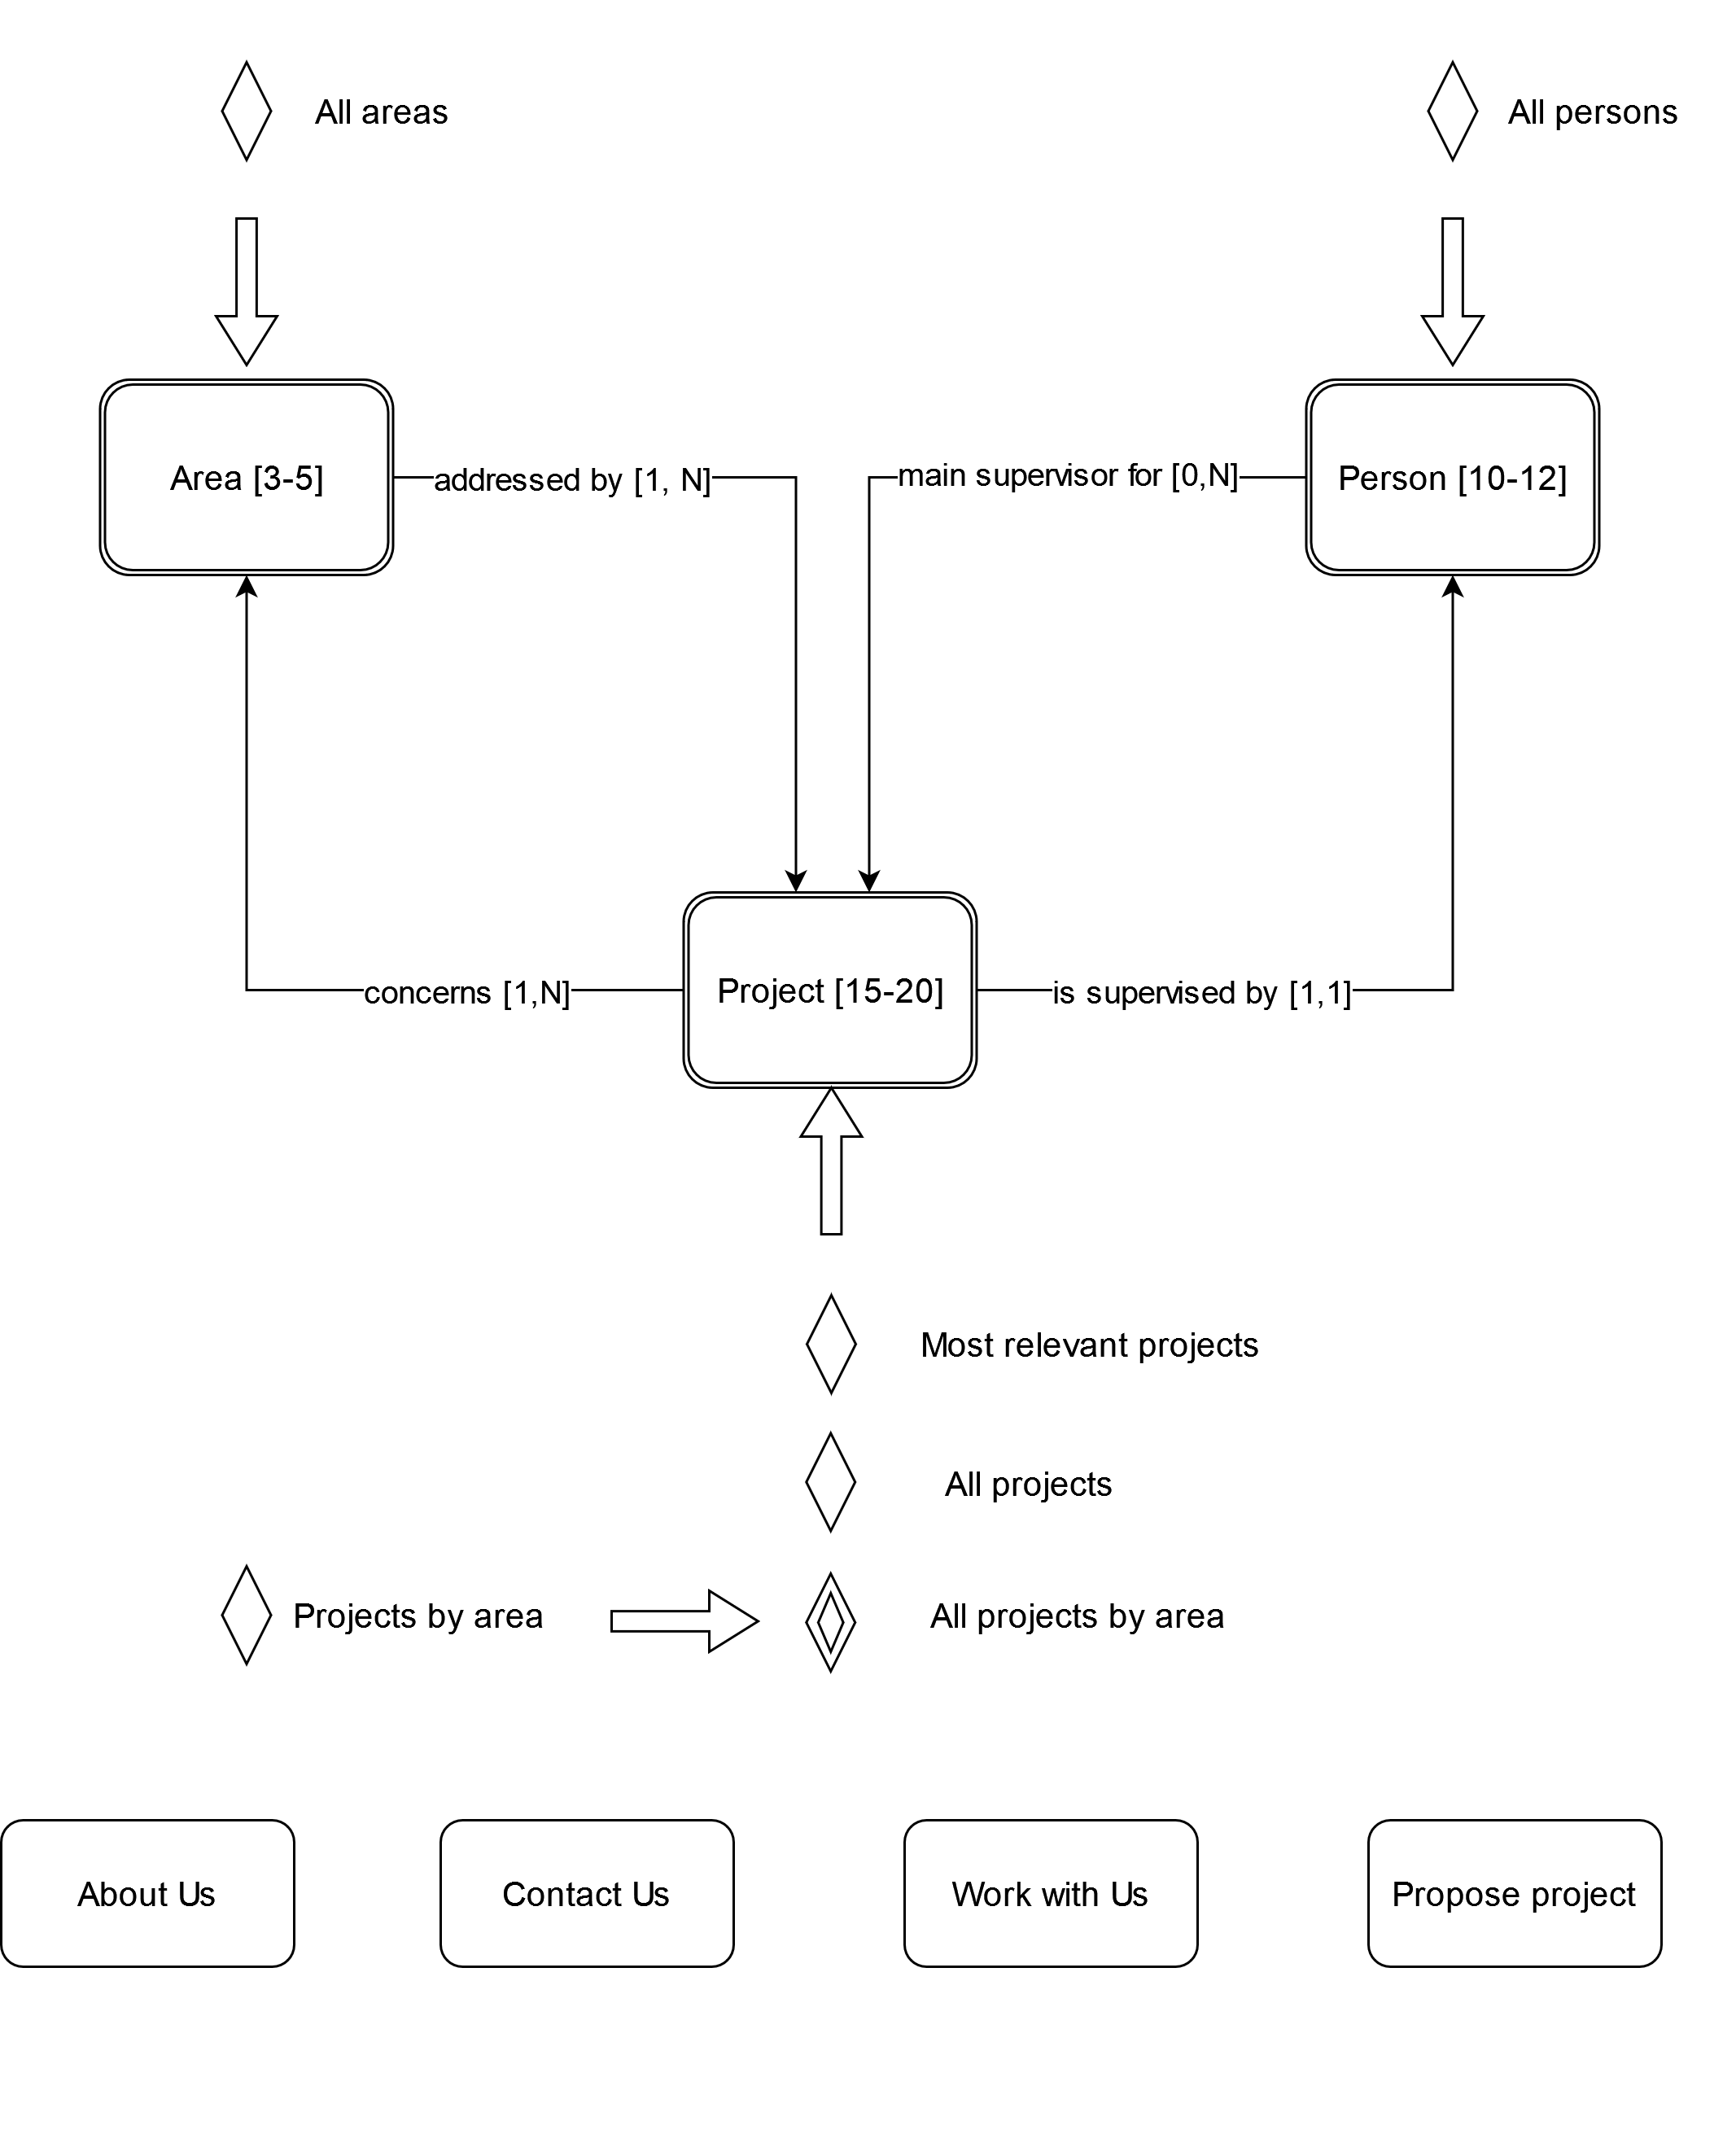
\includegraphics[width=15cm]{images/Hyper_Design-C-IDM.png}
    \caption{C-IDM Diagram}
    \label{fig:enter-label}
\end{figure}
\section{Content-in-the-small Tables}
\subsection{Areas}
\begin{figure}[H]
    \centering
    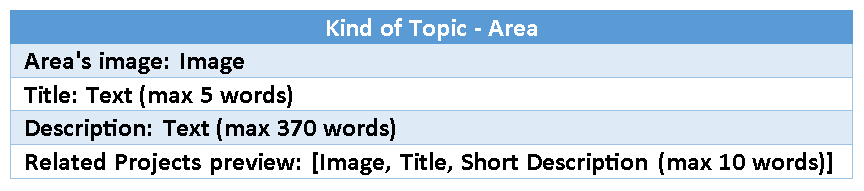
\includegraphics[width=15cm]{images/Content_in_the_small/Kind_of_topic-areas.png}
    \caption{Kind of topic - Area}
    \label{fig:enter-label}
\end{figure}

\begin{figure}[H]
    \centering
    
\includegraphics[width=15cm]{images/Content_in_the_small/Group-All_areas.png}
    \caption{Group - All areas}
    \label{fig:enter-label}
\end{figure}

\subsection{Persons}
\begin{figure}[H]
    \centering
    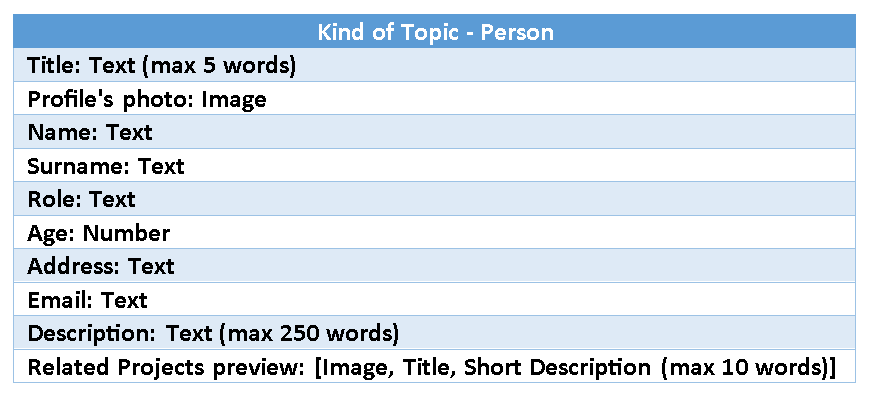
\includegraphics[width=15cm]{images/Content_in_the_small/Kind_of_topic-person.png}
    \caption{Kind of topic - Person}
    \label{fig:enter-label}
\end{figure}
\begin{figure}[H]
    \centering
    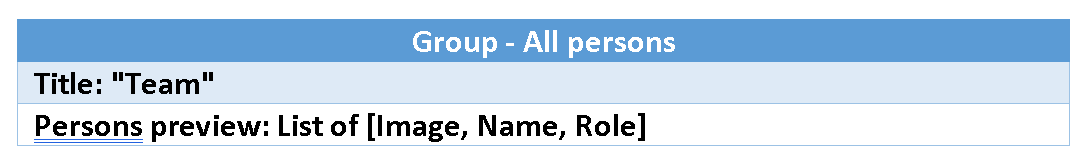
\includegraphics[width=15cm]{images/Content_in_the_small/Group-All_person.png}
    \caption{Group - All persons}
    \label{fig:enter-label}
\end{figure}

\subsection{Projects}
\begin{figure}[H]
    \centering
    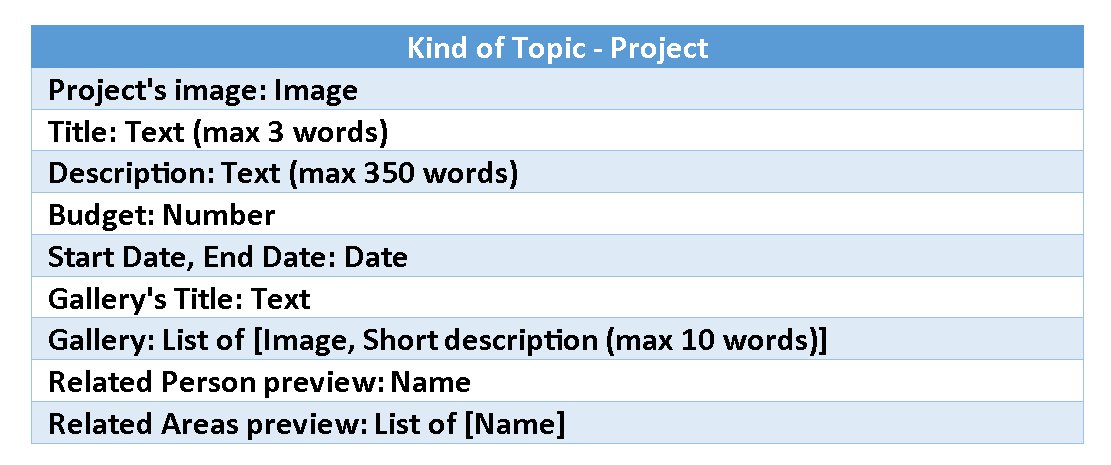
\includegraphics[width=15cm]{images/Content_in_the_small/Kind_of_topic-Project.png}
    \caption{Kind of topic - Project}
    \label{fig:enter-label}
\end{figure}
\begin{figure}[H]
    \centering
    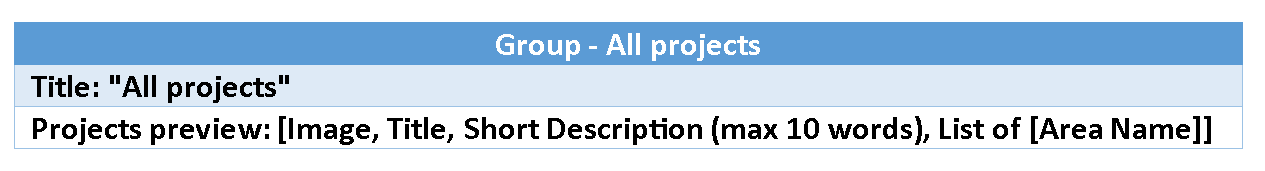
\includegraphics[width=15cm]{images/Content_in_the_small/Group-All_projects.png}
    \caption{Group - All projects}
    \label{fig:enter-label}
\end{figure}
\begin{figure}[H]
    \centering
    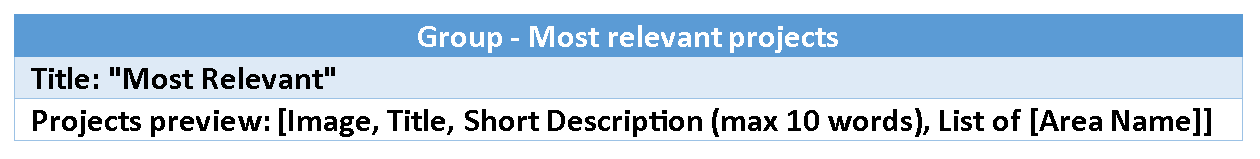
\includegraphics[width=15cm]{images/Content_in_the_small/Group-Most_relevant_projects.png}
    \caption{Group - Most relevant projects}
    \label{fig:enter-label}
\end{figure}
\begin{figure}[H]
    \centering
    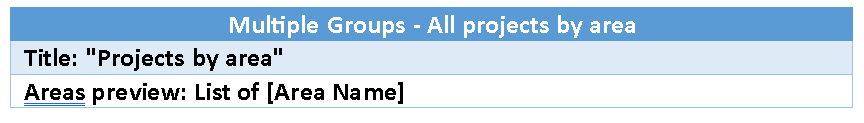
\includegraphics[width=15cm]{images/Content_in_the_small/Mutiple_gruop-all_projects_by_area.png}
    \caption{Multiple group - All projects by area}
    \label{fig:enter-label}
\end{figure}

\begin{figure}[H]
    \centering
    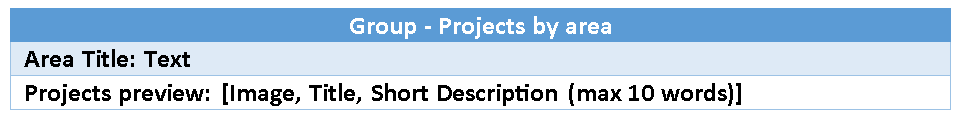
\includegraphics[width=15cm]{images/Content_in_the_small/Group-Projects_by_area.png}
    \caption{Group - Projects by area}
    \label{fig:enter-label}
\end{figure}

\subsection{About us}
\begin{figure}[H]
    \centering
    
\includegraphics[width=15cm]{images/Content_in_the_small/Topic-About_us.png}
    \caption{Topic - About Us}
    \label{fig:enter-label}
\end{figure}

\subsection{Contact us}
\begin{figure}[H]
    \centering
    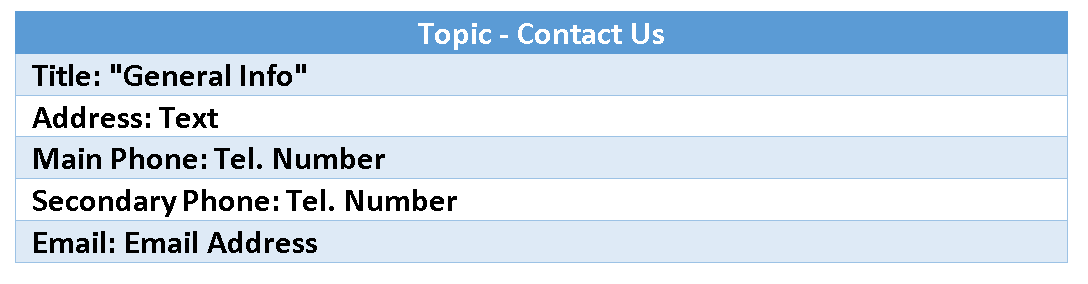
\includegraphics[width=15cm]{images/Content_in_the_small/Topic-contact_us.png}
    \caption{Topic - Contact Us}
    \label{fig:enter-label}
\end{figure}

\begin{figure}[H]
    \centering
    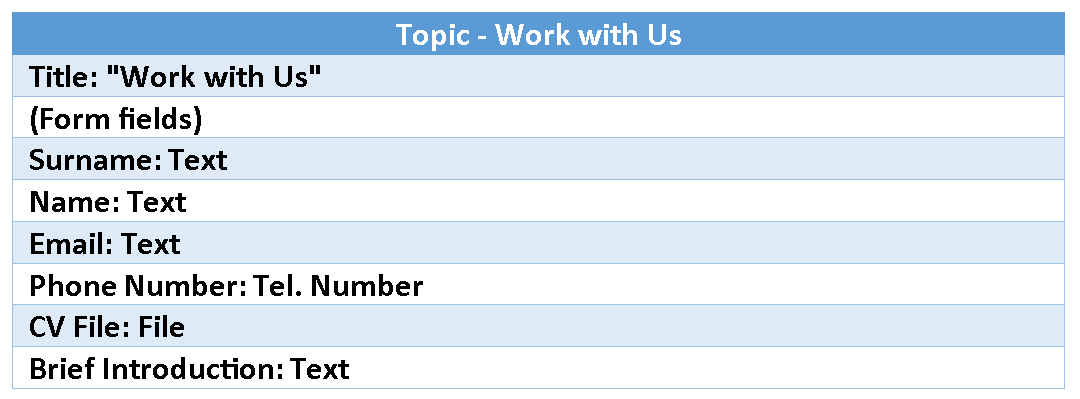
\includegraphics[width=15cm]{images/Content_in_the_small/Topic-work-with-us.png}
    \caption{Topic - Work with Us}
    \label{fig:enter-label}
\end{figure}
\begin{figure}[H]
    \centering
    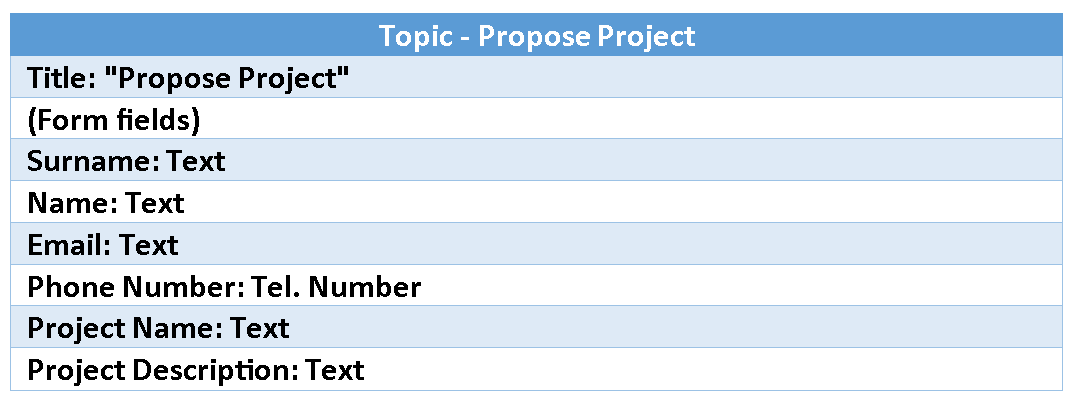
\includegraphics[width=15cm]{images/Content_in_the_small/Topic-propose_project.png}
    \caption{Topic - Propose Project}
    \label{fig:enter-label}
\end{figure}

\label{sec:final_commented_wireframes}
\section{Final Commented Wireframes}
This section contains high-fidelity screenshots of the different types of pages of the website, with comments about the connectivity and the different links.
\\
\\
Important notes: 
\begin{itemize}
    \item The header and the footer are always present, so their link analysis that is done only in the homepage will be valid for all the website.
    \item The orientation info in the Kind of Topic pages (Area, Person, Project) is missing due to implementation reasons. They were planned from the design point of view, in the same way they are present in all the other pages, but we weren't able to properly implement them in Nuxt. For example, in "Areas", "Projects", "Team", "About Us" and "Contact Us" the section is correctly highlighted; instead, when inside a single area, or project, or person, the orientation info disappears. We notify this for consistency reasons.
\end{itemize}

\subsubsection*{Homepage}
\begin{figure}[H]
    \centering
    \setlength{\fboxsep}{0pt}\fbox{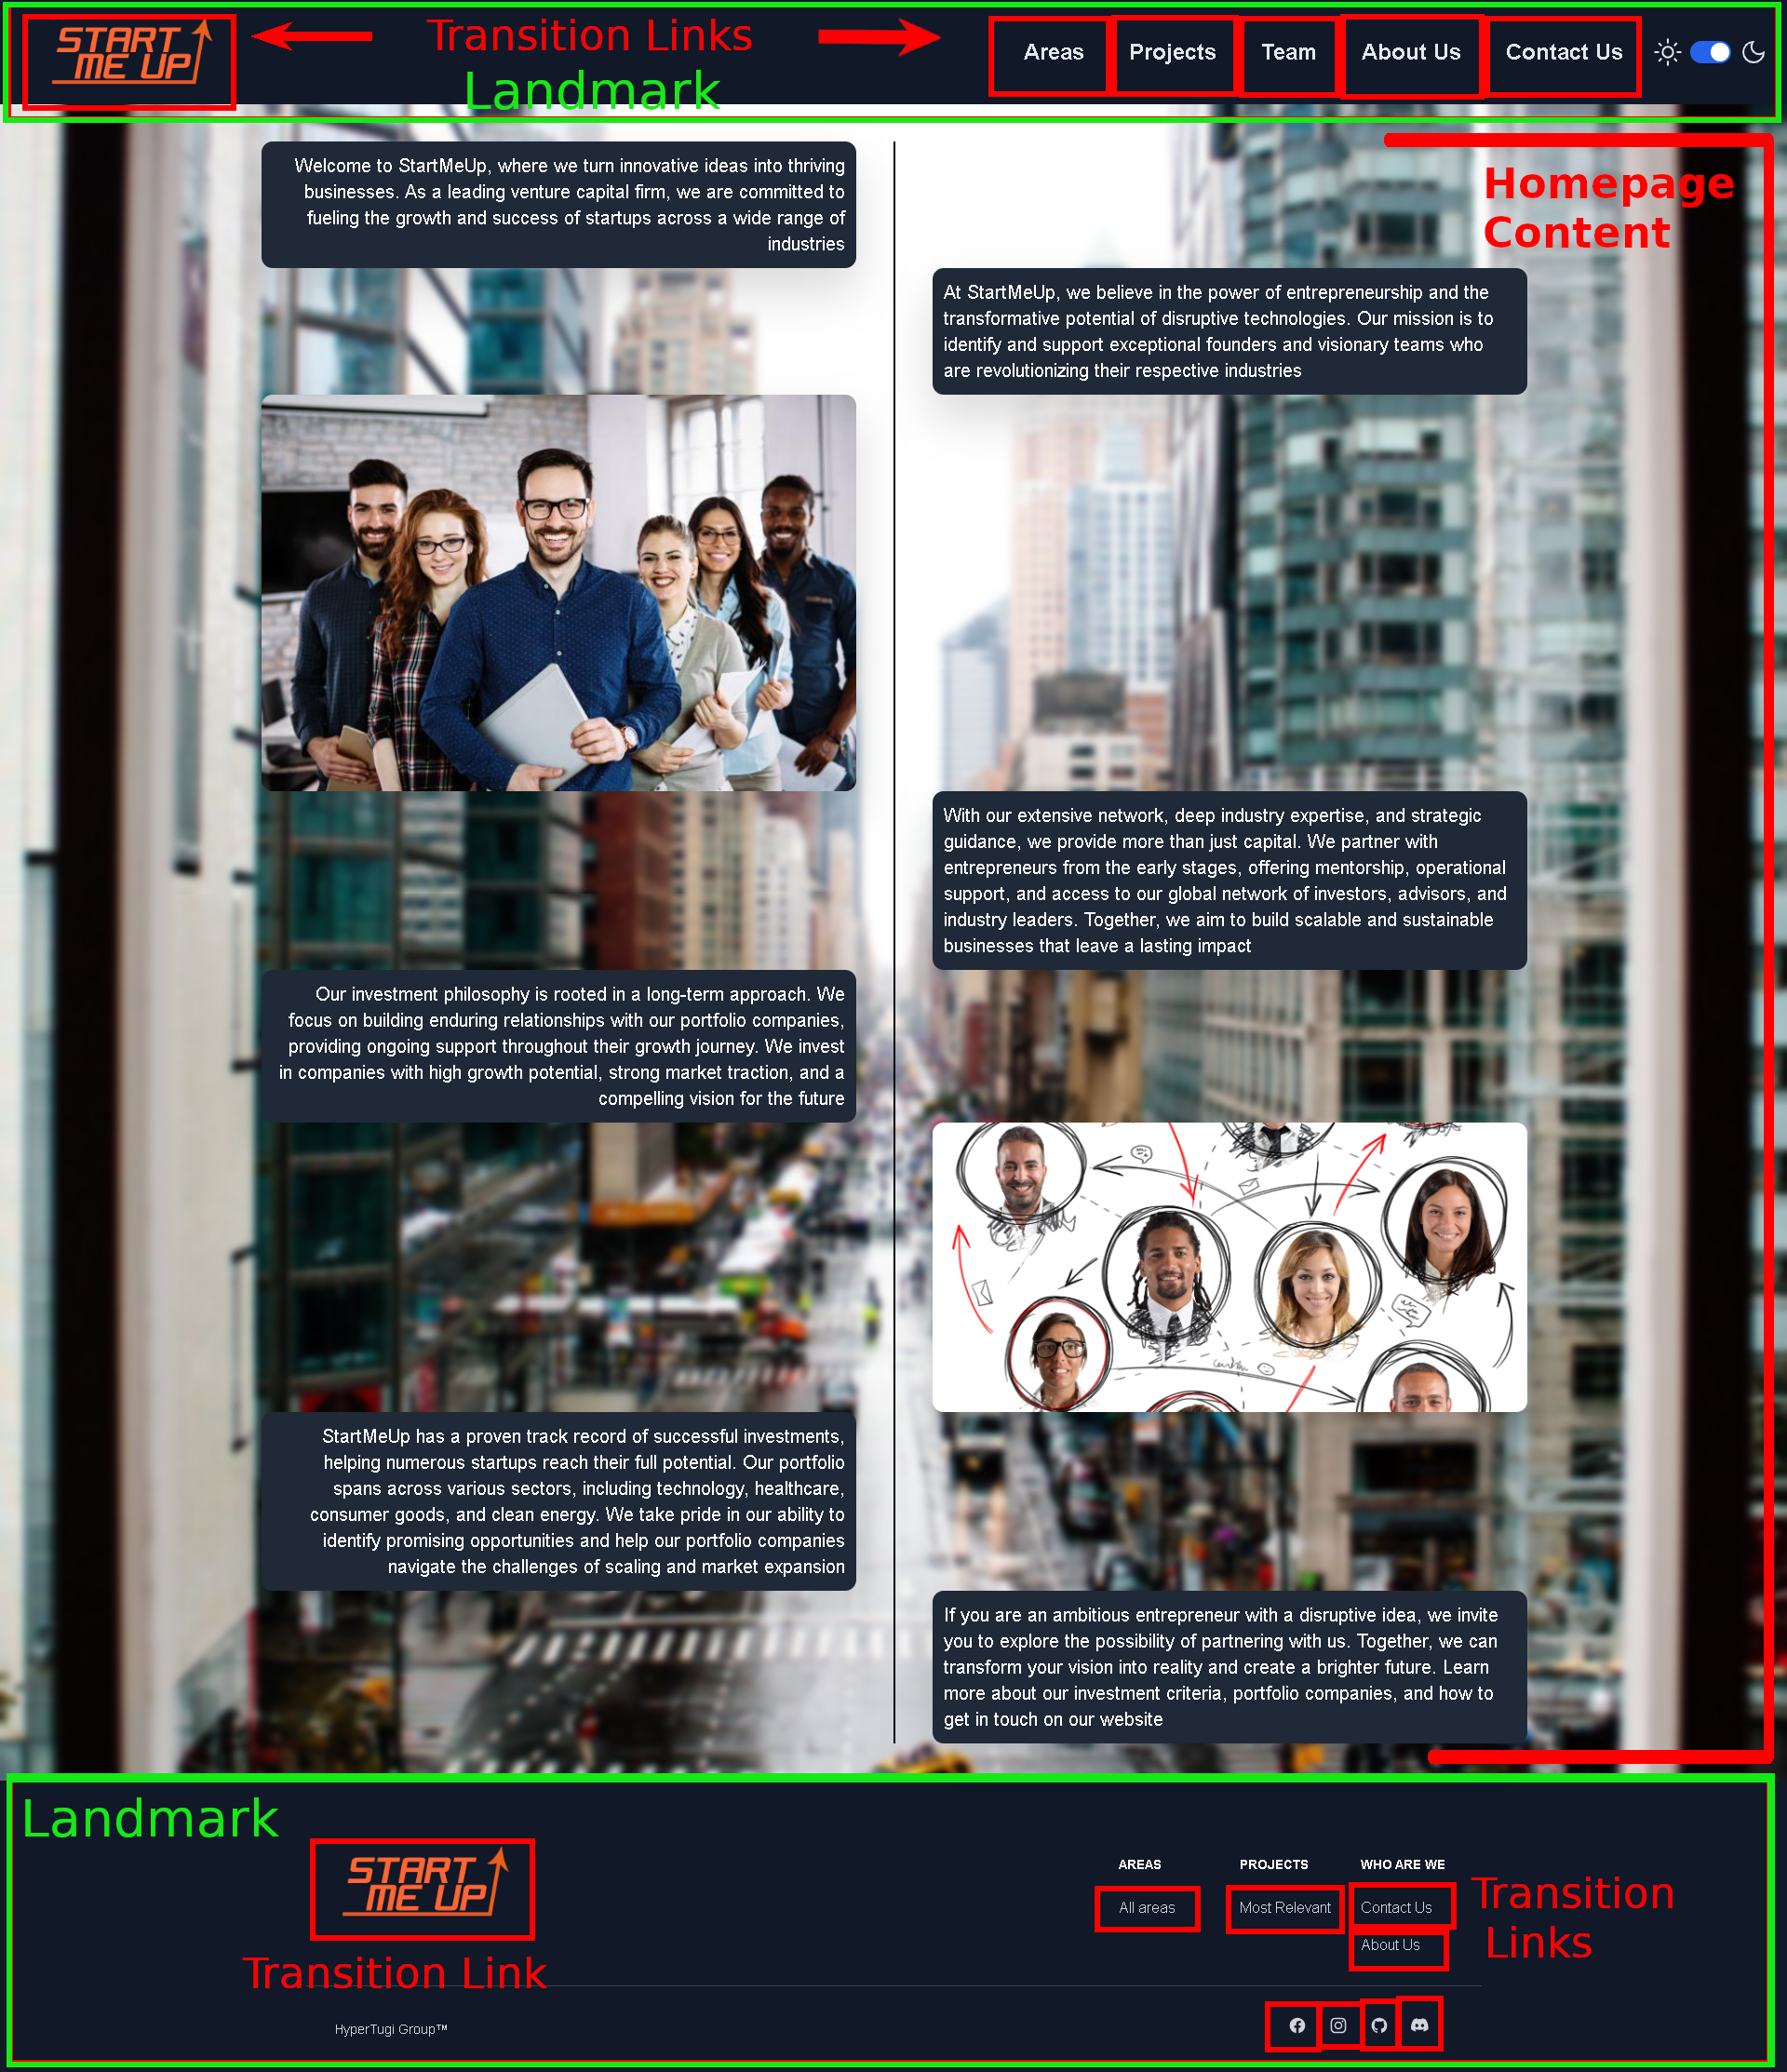
\includegraphics[width=14cm]{images/Pages Screenshots/Homepage.png}}
    \caption{Homepage - High-fidelity screenshot}
    \label{fig:PageScreenshot_Homepage}
\end{figure}

\subsection{Areas}

\subsubsection*{Area}
\begin{figure}[H]
    \centering
    \setlength{\fboxsep}{0pt}\fbox{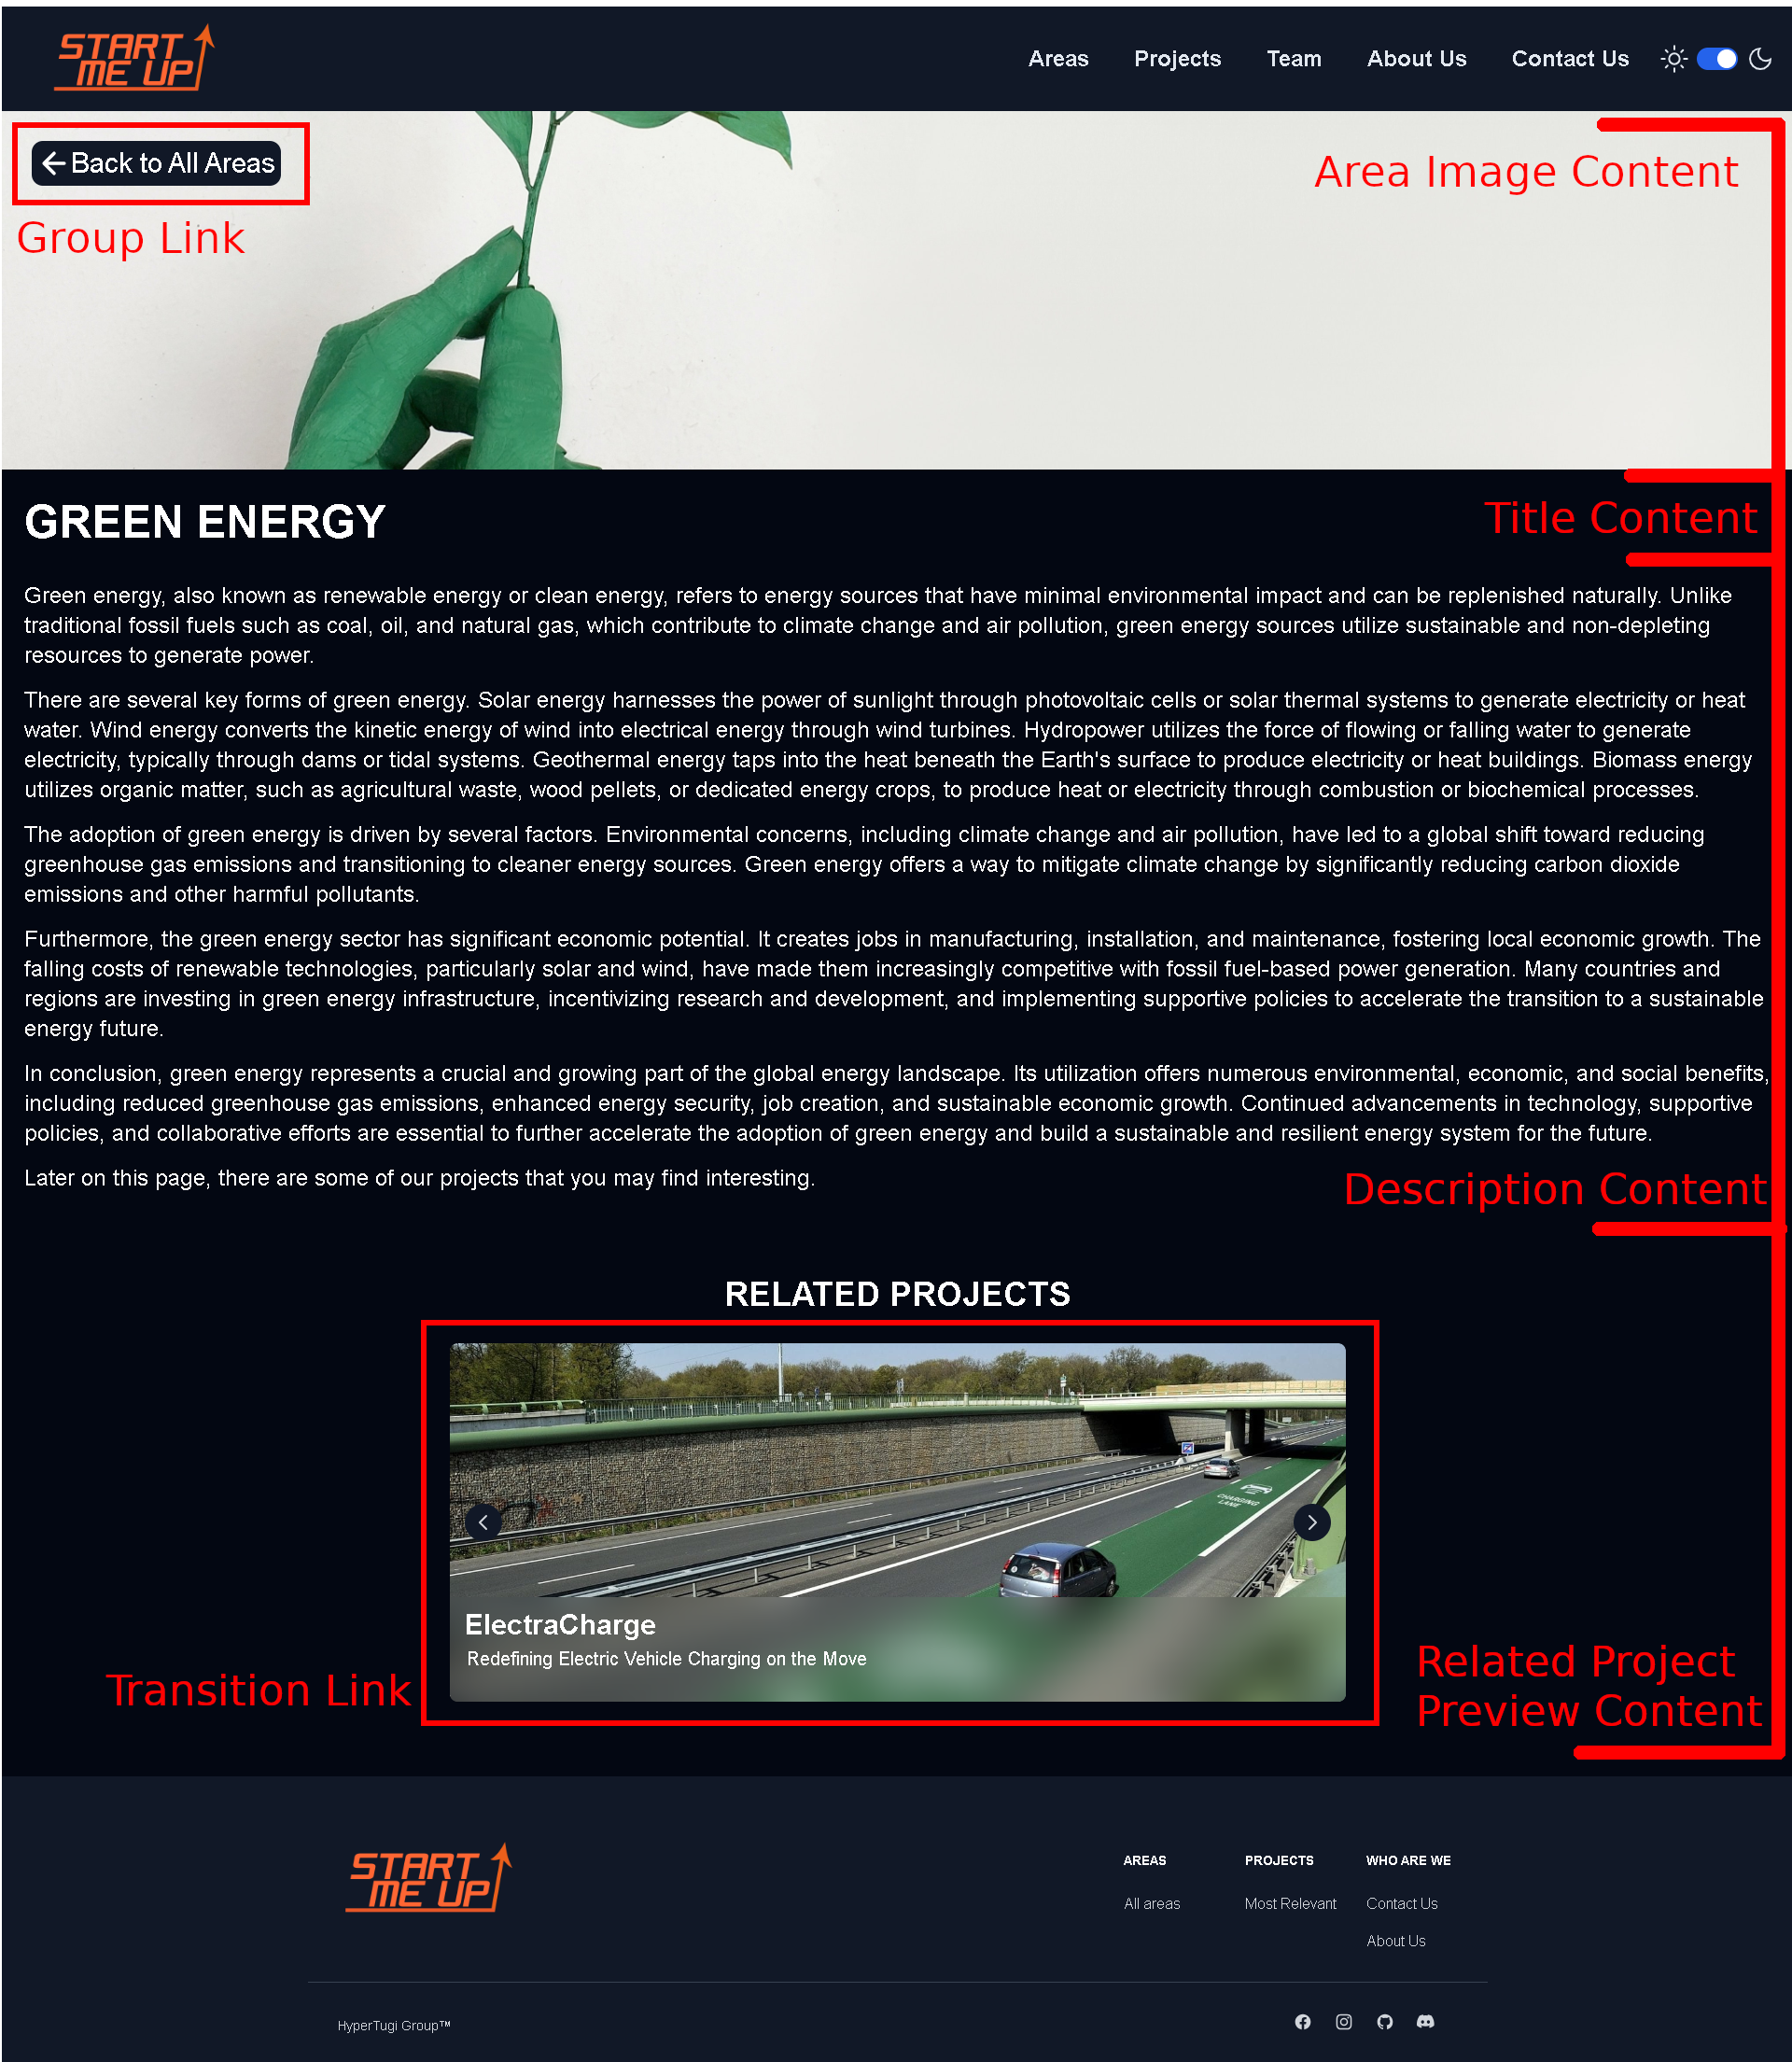
\includegraphics[width=16cm]{images/Pages Screenshots/Area.png}}
    \caption{Area - High-fidelity screenshot}
    \label{fig:PageScreenshot_Area}
\end{figure}

\subsubsection*{All Areas}
\begin{figure}[H]
    \centering
    \setlength{\fboxsep}{0pt}\fbox{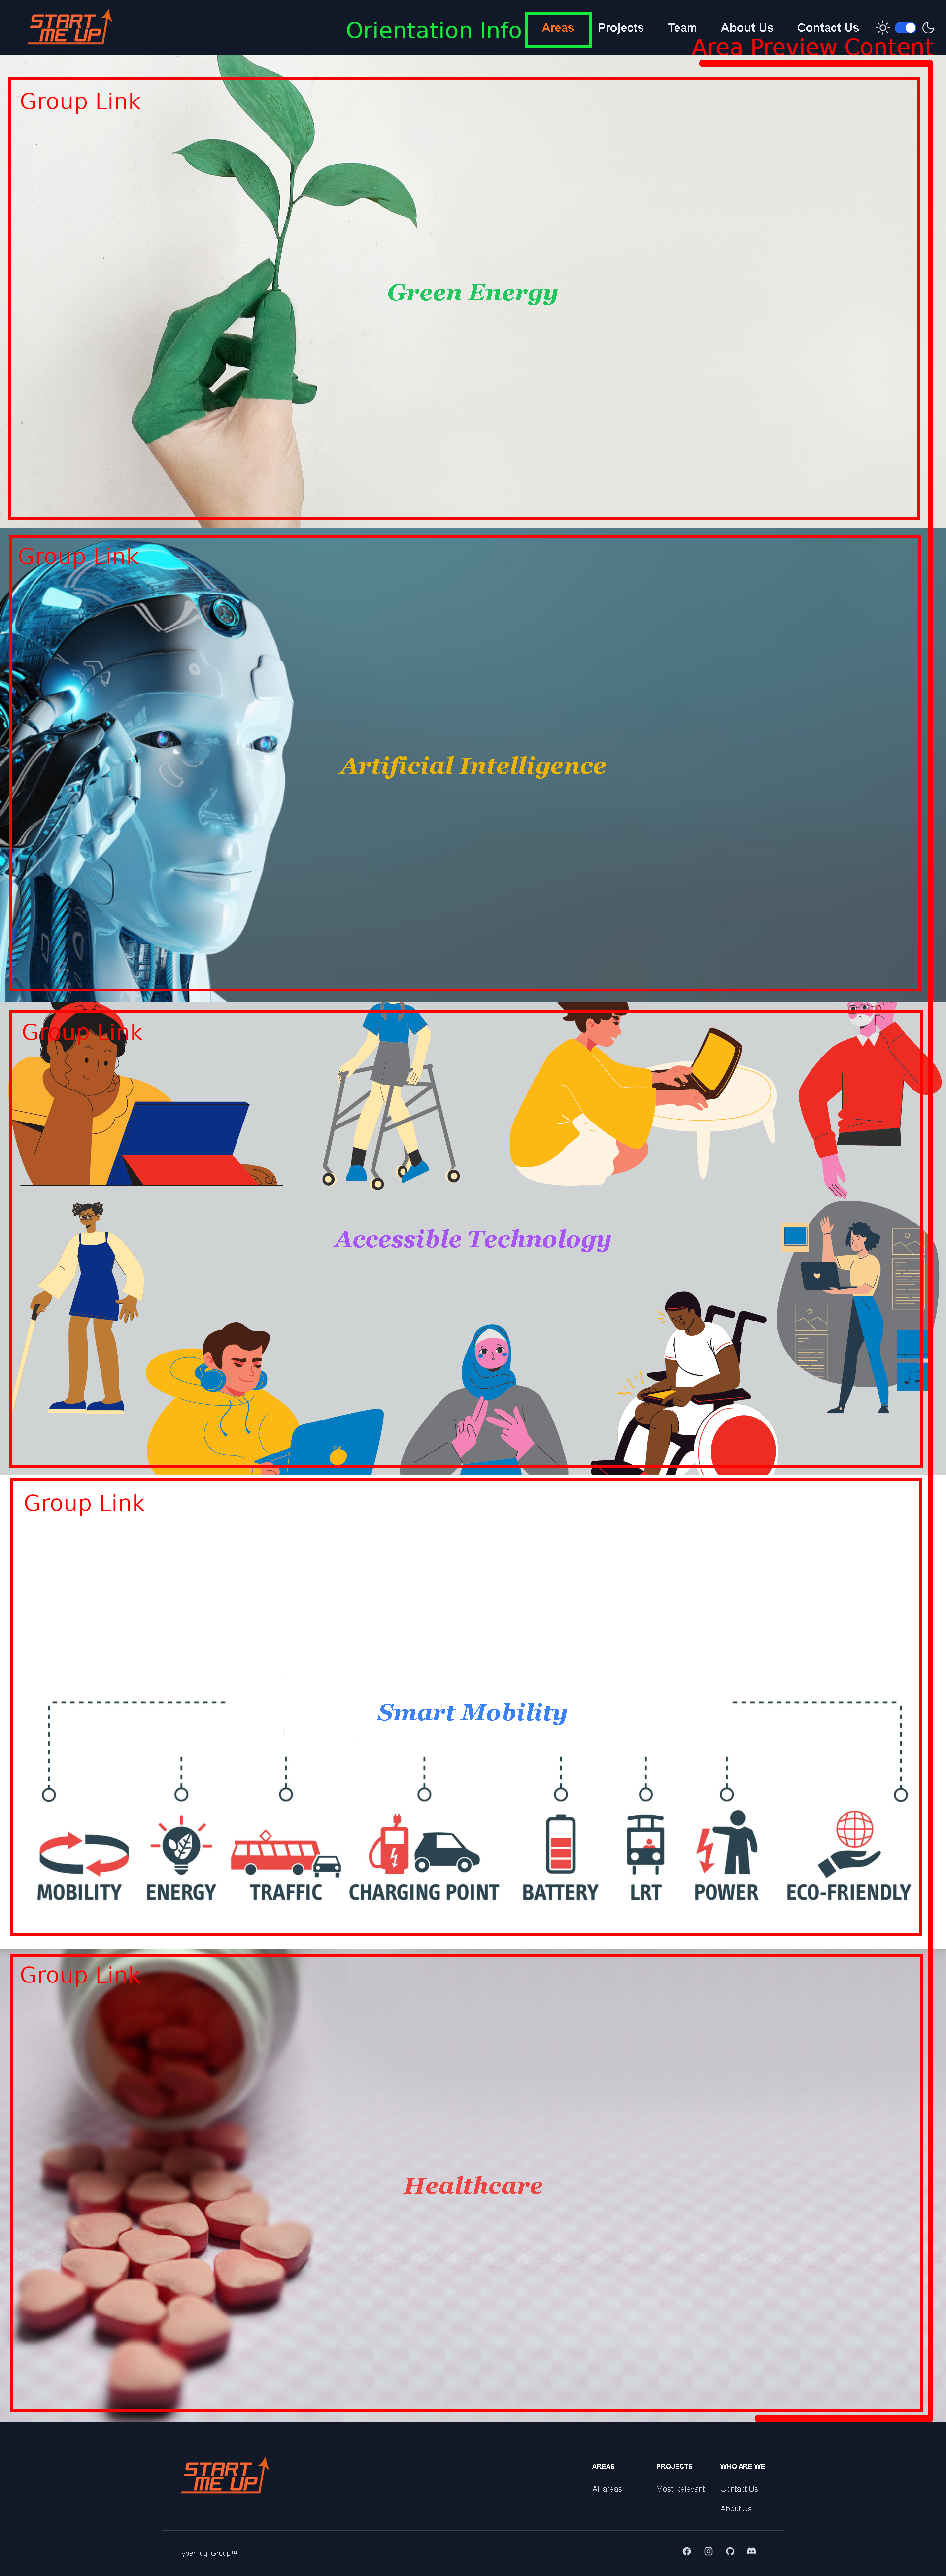
\includegraphics[width=8cm]{images/Pages Screenshots/Areas.png}}
    \caption{All Areas - High-fidelity screenshot}
    \label{fig:PageScreenshot_All_areas}
\end{figure}

\subsection{Persons}

\subsubsection*{Person}
\begin{figure}[H]
    \centering
    \setlength{\fboxsep}{0pt}\fbox{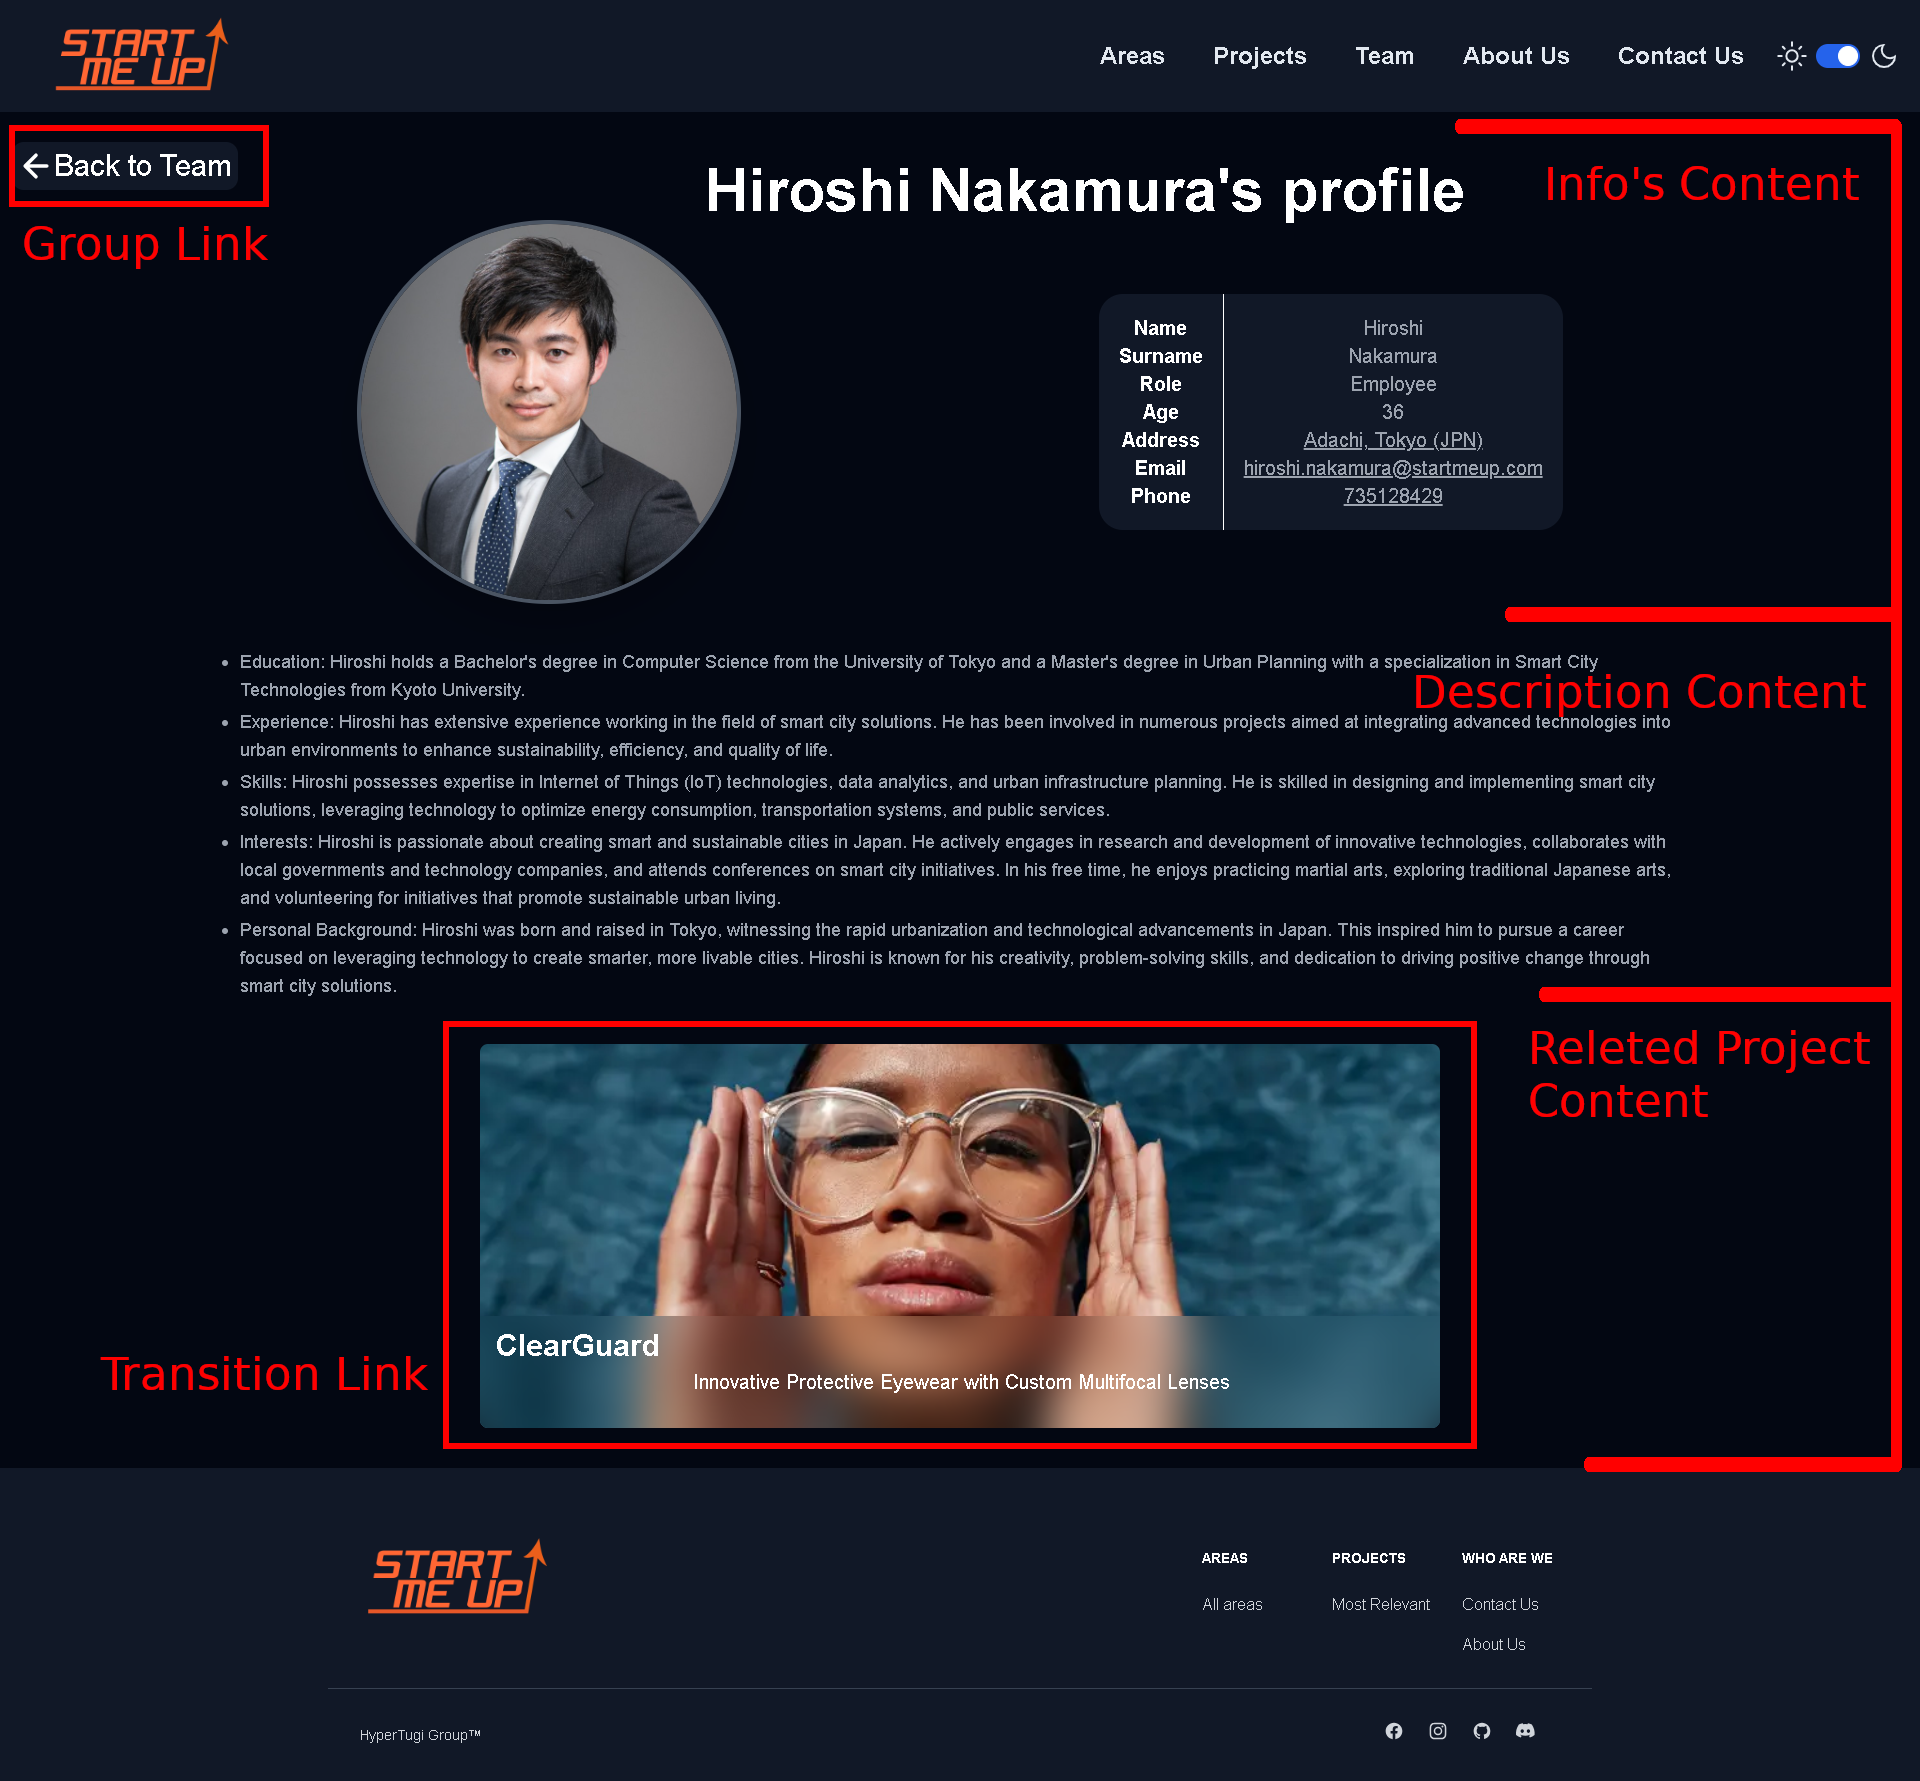
\includegraphics[width=16cm]{images/Pages Screenshots/Person.png}}
    \caption{Person - High-fidelity screenshot}
    \label{fig:PageScreenshot_Person}
\end{figure}

\subsubsection*{All persons}
\label{sec:wrong_blurred_box}
\begin{figure}[H]
    \centering
    \setlength{\fboxsep}{0pt}\fbox{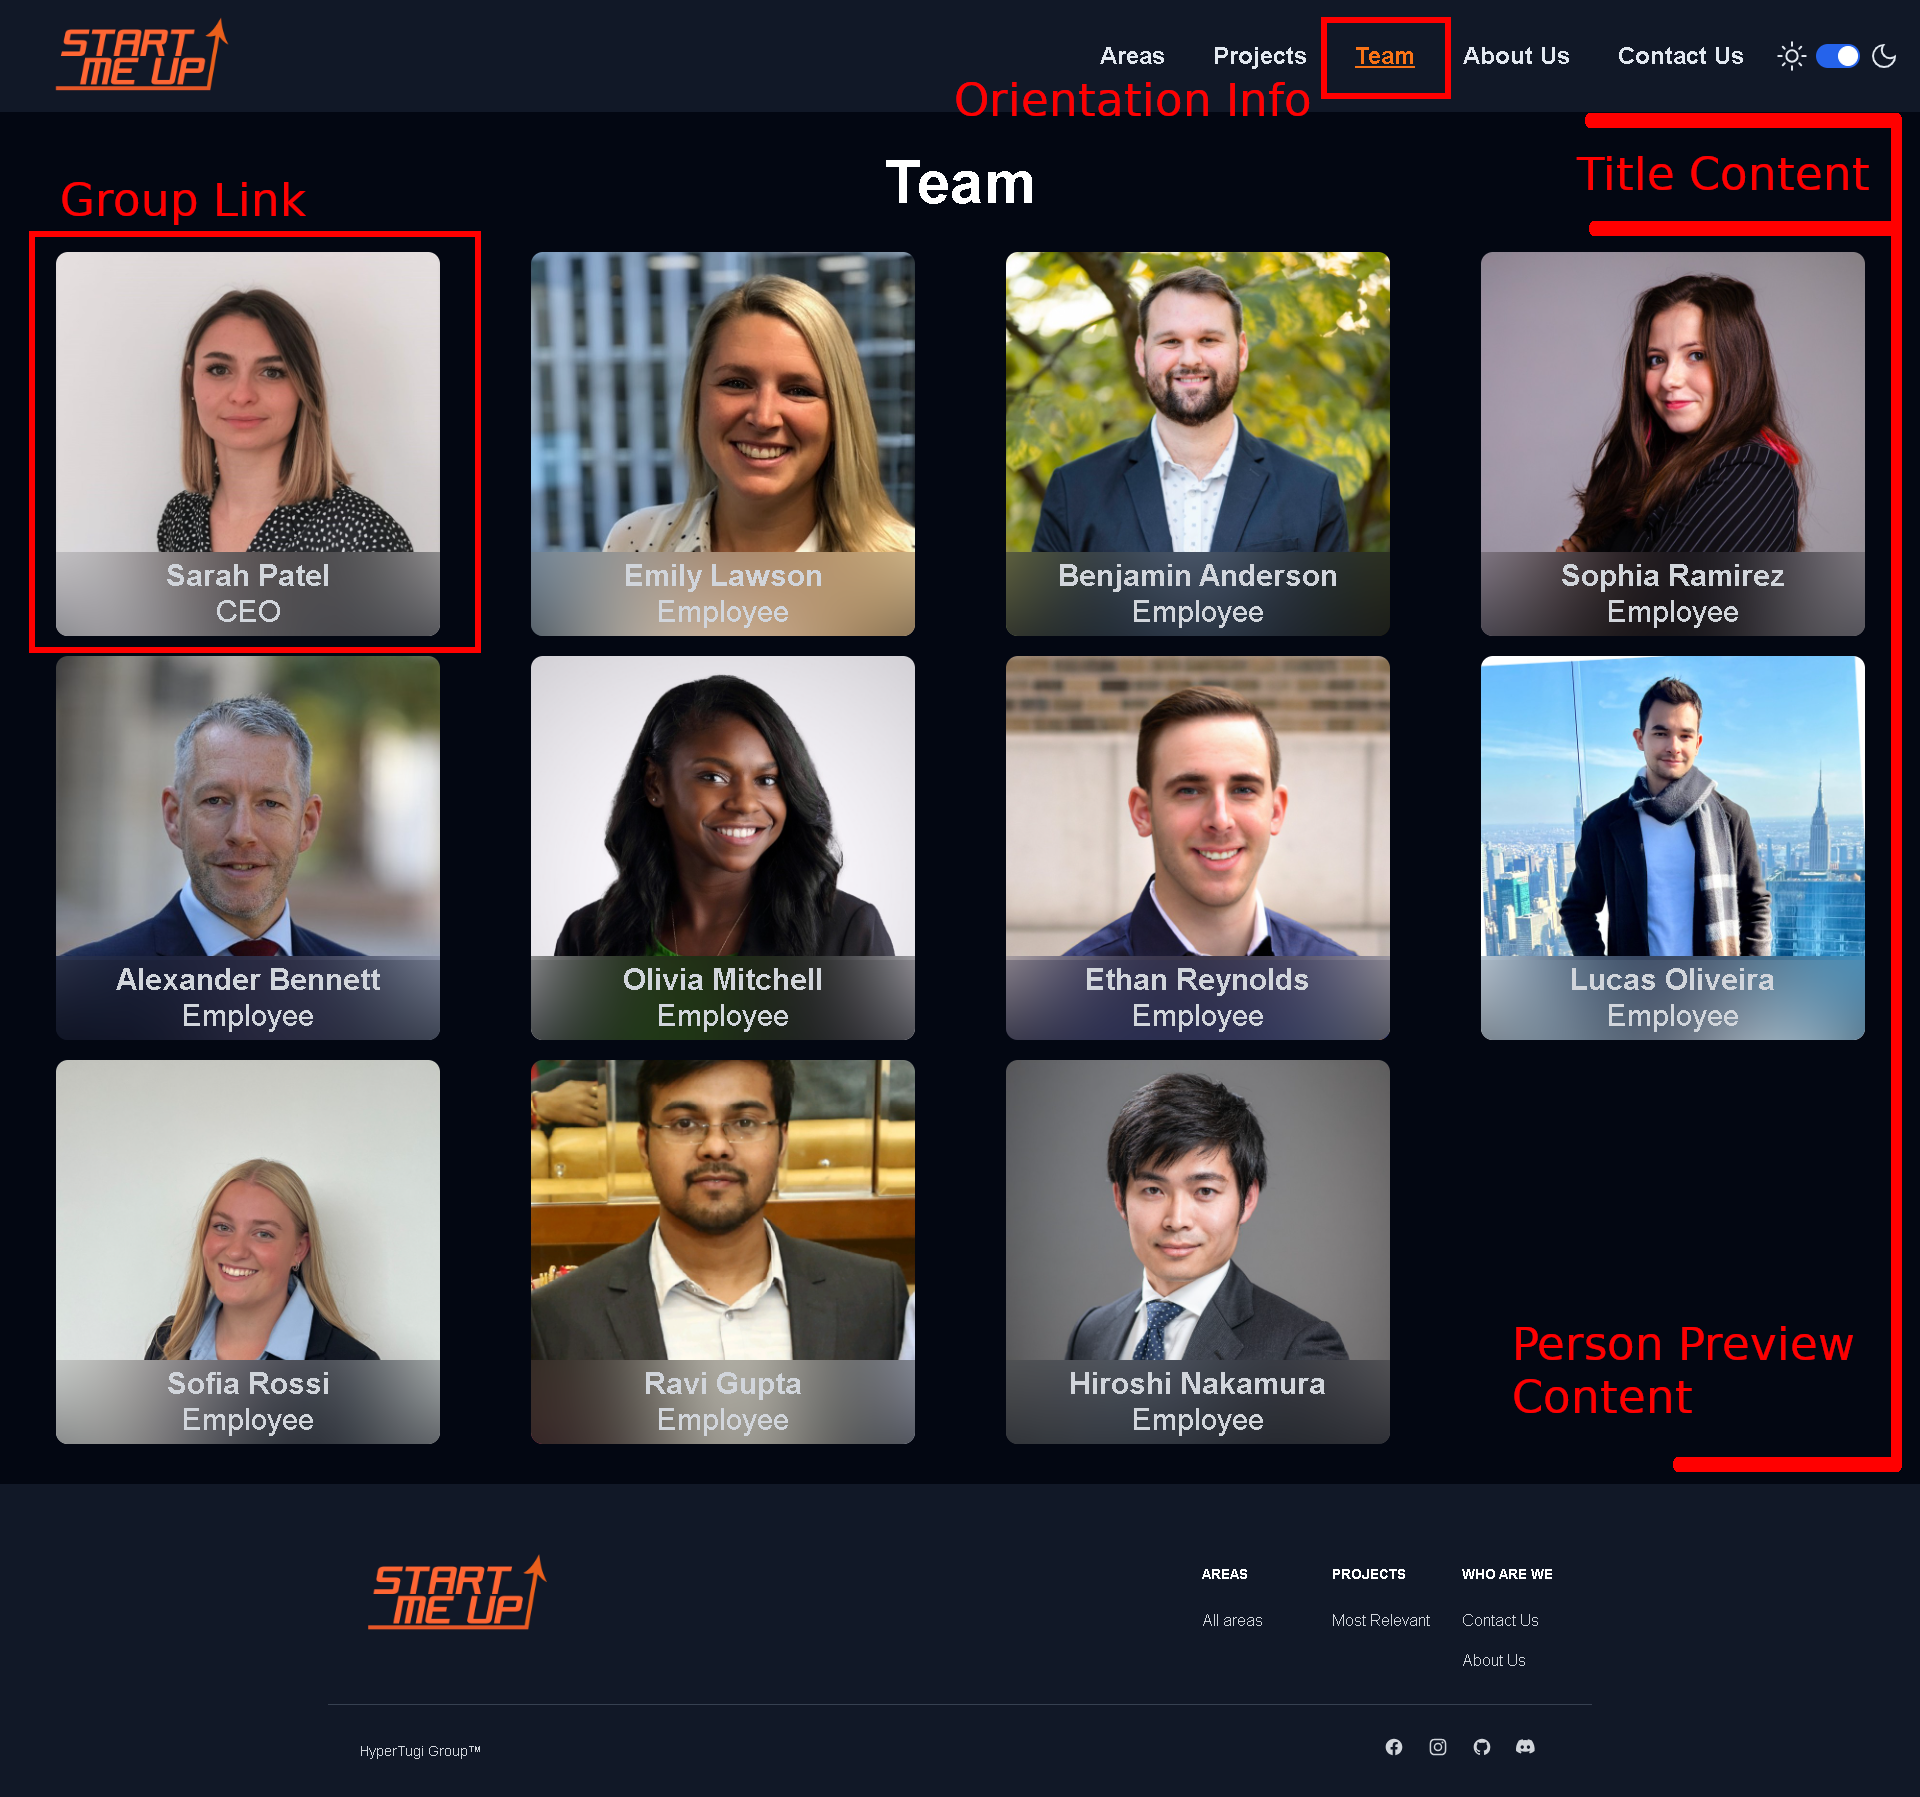
\includegraphics[width=16cm]{images/Pages Screenshots/Team.png}}
    \caption{All persons - High-fidelity screenshot}
    \label{fig:PageScreenshot_All_persons}
\end{figure}

\subsection{Projects}

\subsubsection*{Project}
\begin{figure}[H]
    \centering
    \setlength{\fboxsep}{0pt}\fbox{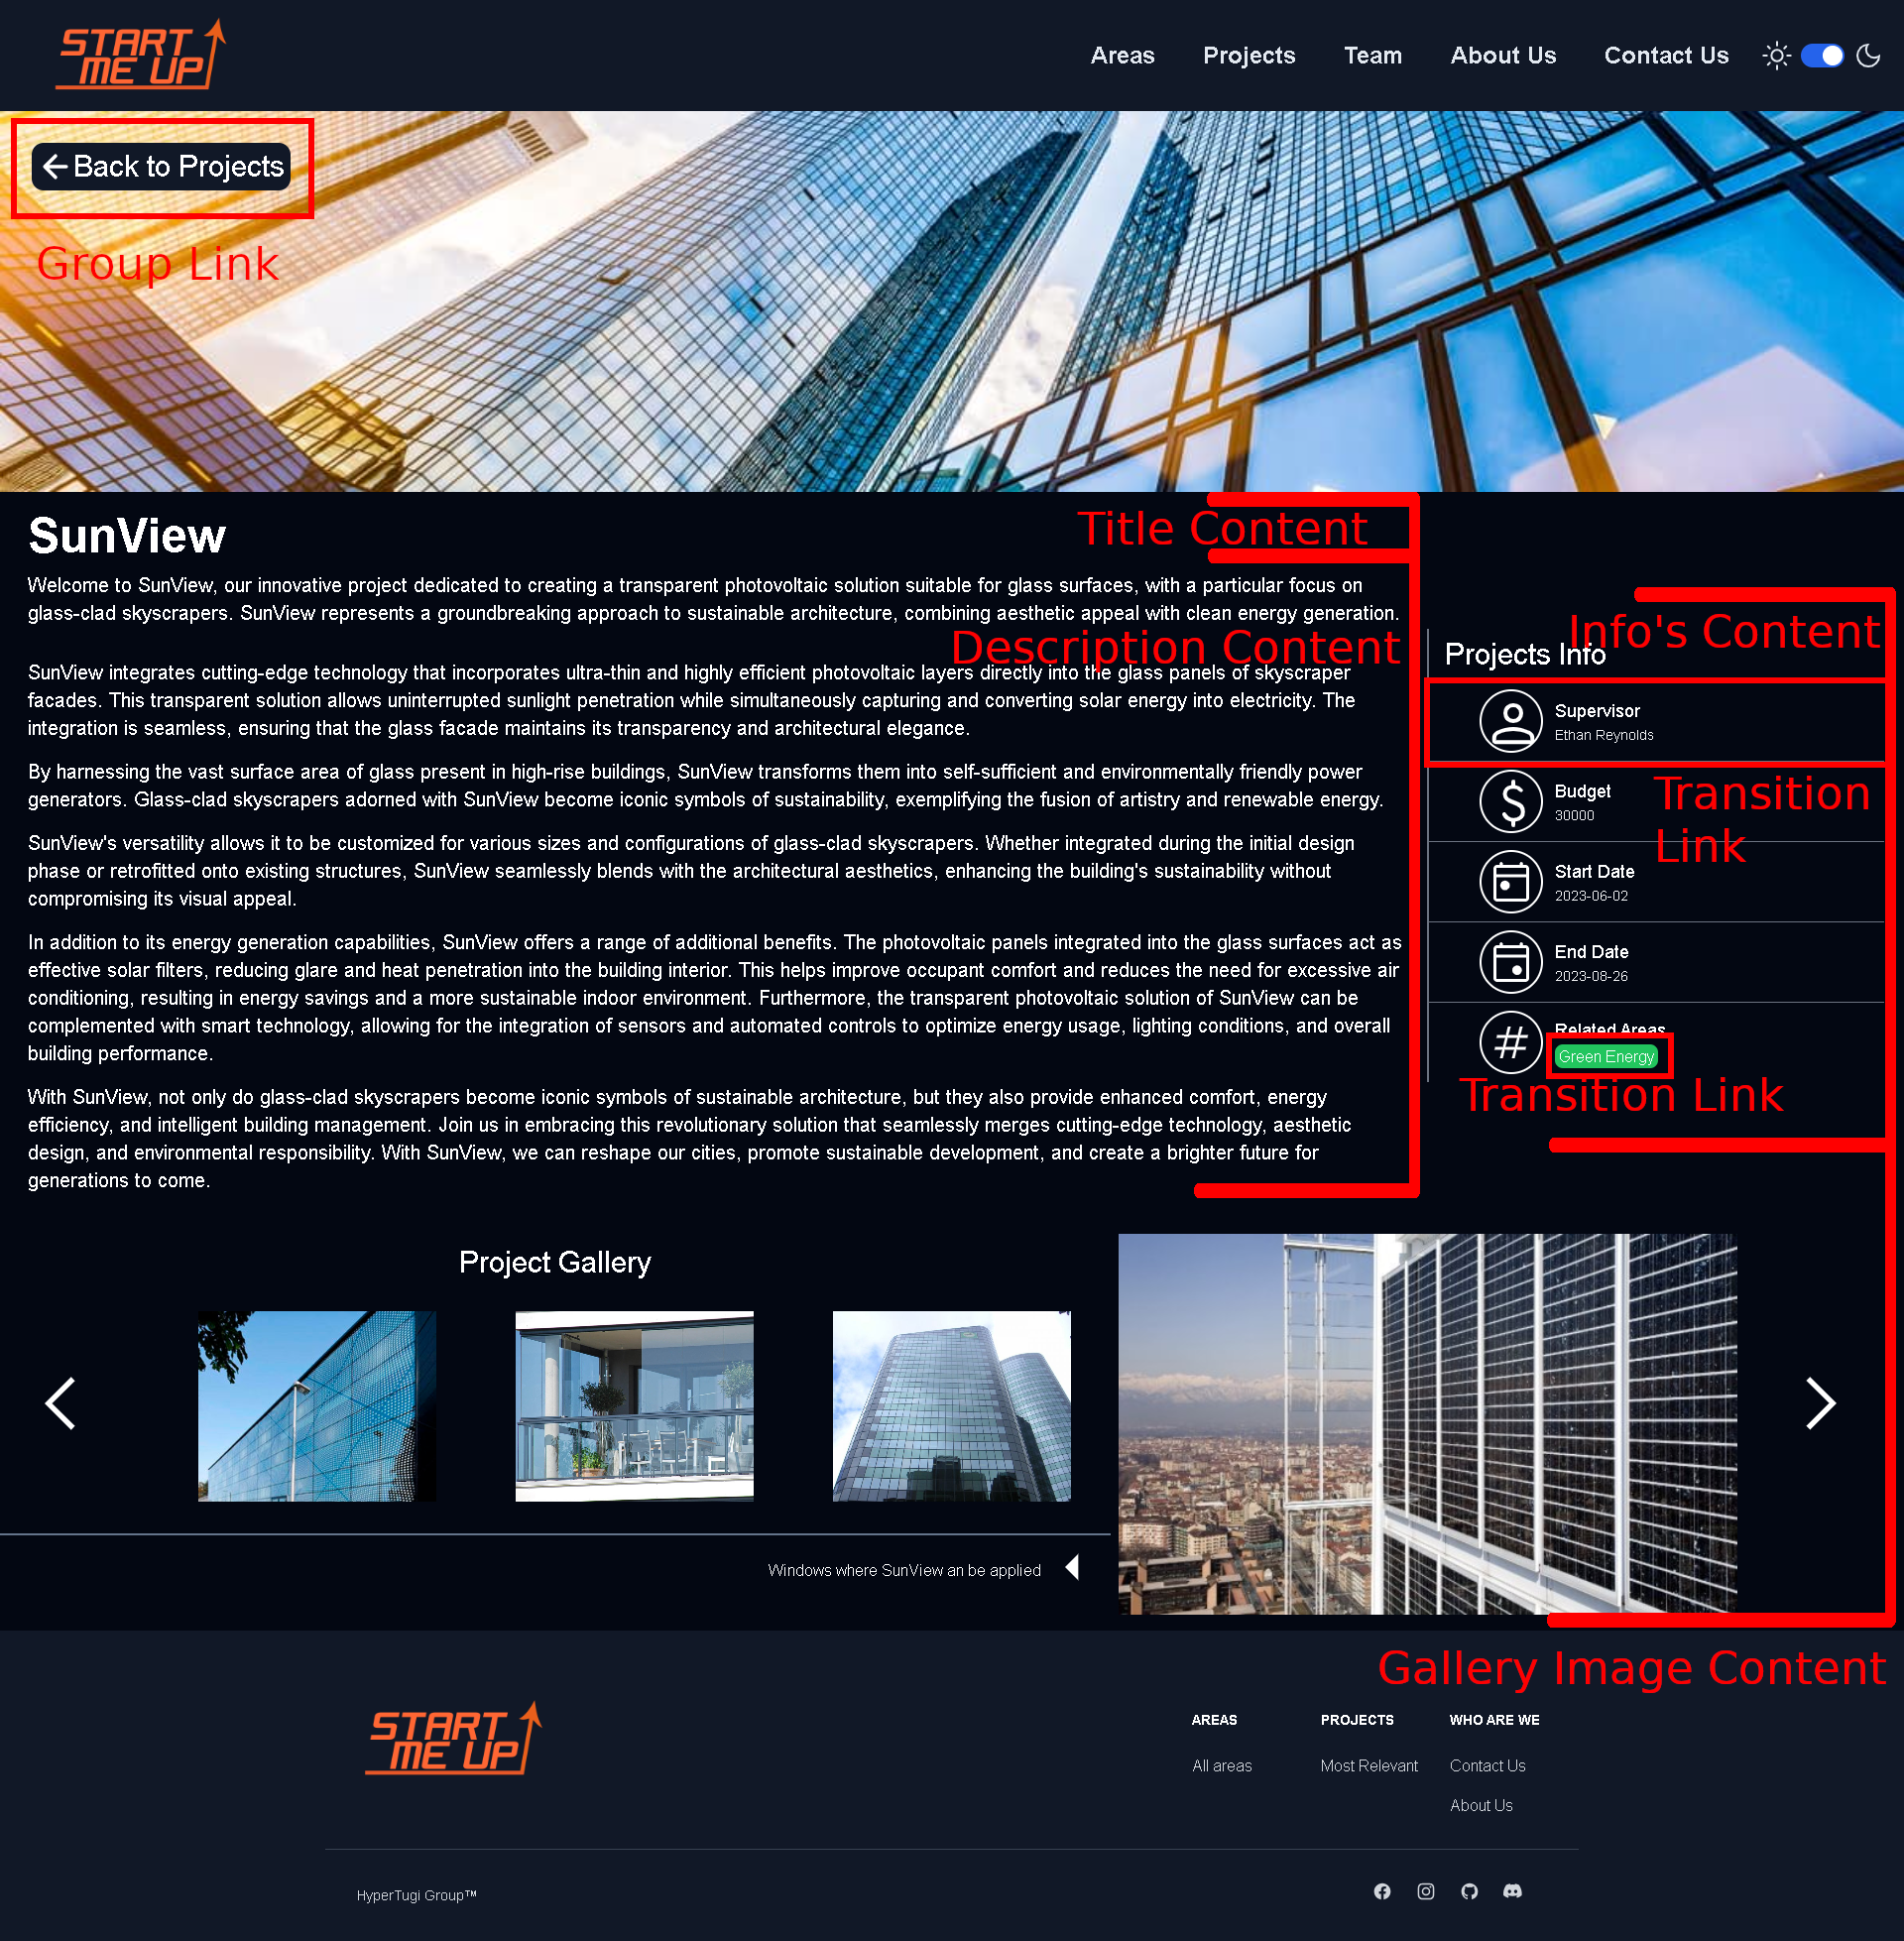
\includegraphics[width=16cm]{images/Pages Screenshots/Project.png}}
    \caption{Project - High-fidelity screenshot}
    \label{fig:PageScreenshot_Project}
\end{figure}

\subsubsection*{Most relevant projects}
\begin{figure}[H]
    \centering
    \setlength{\fboxsep}{0pt}\fbox{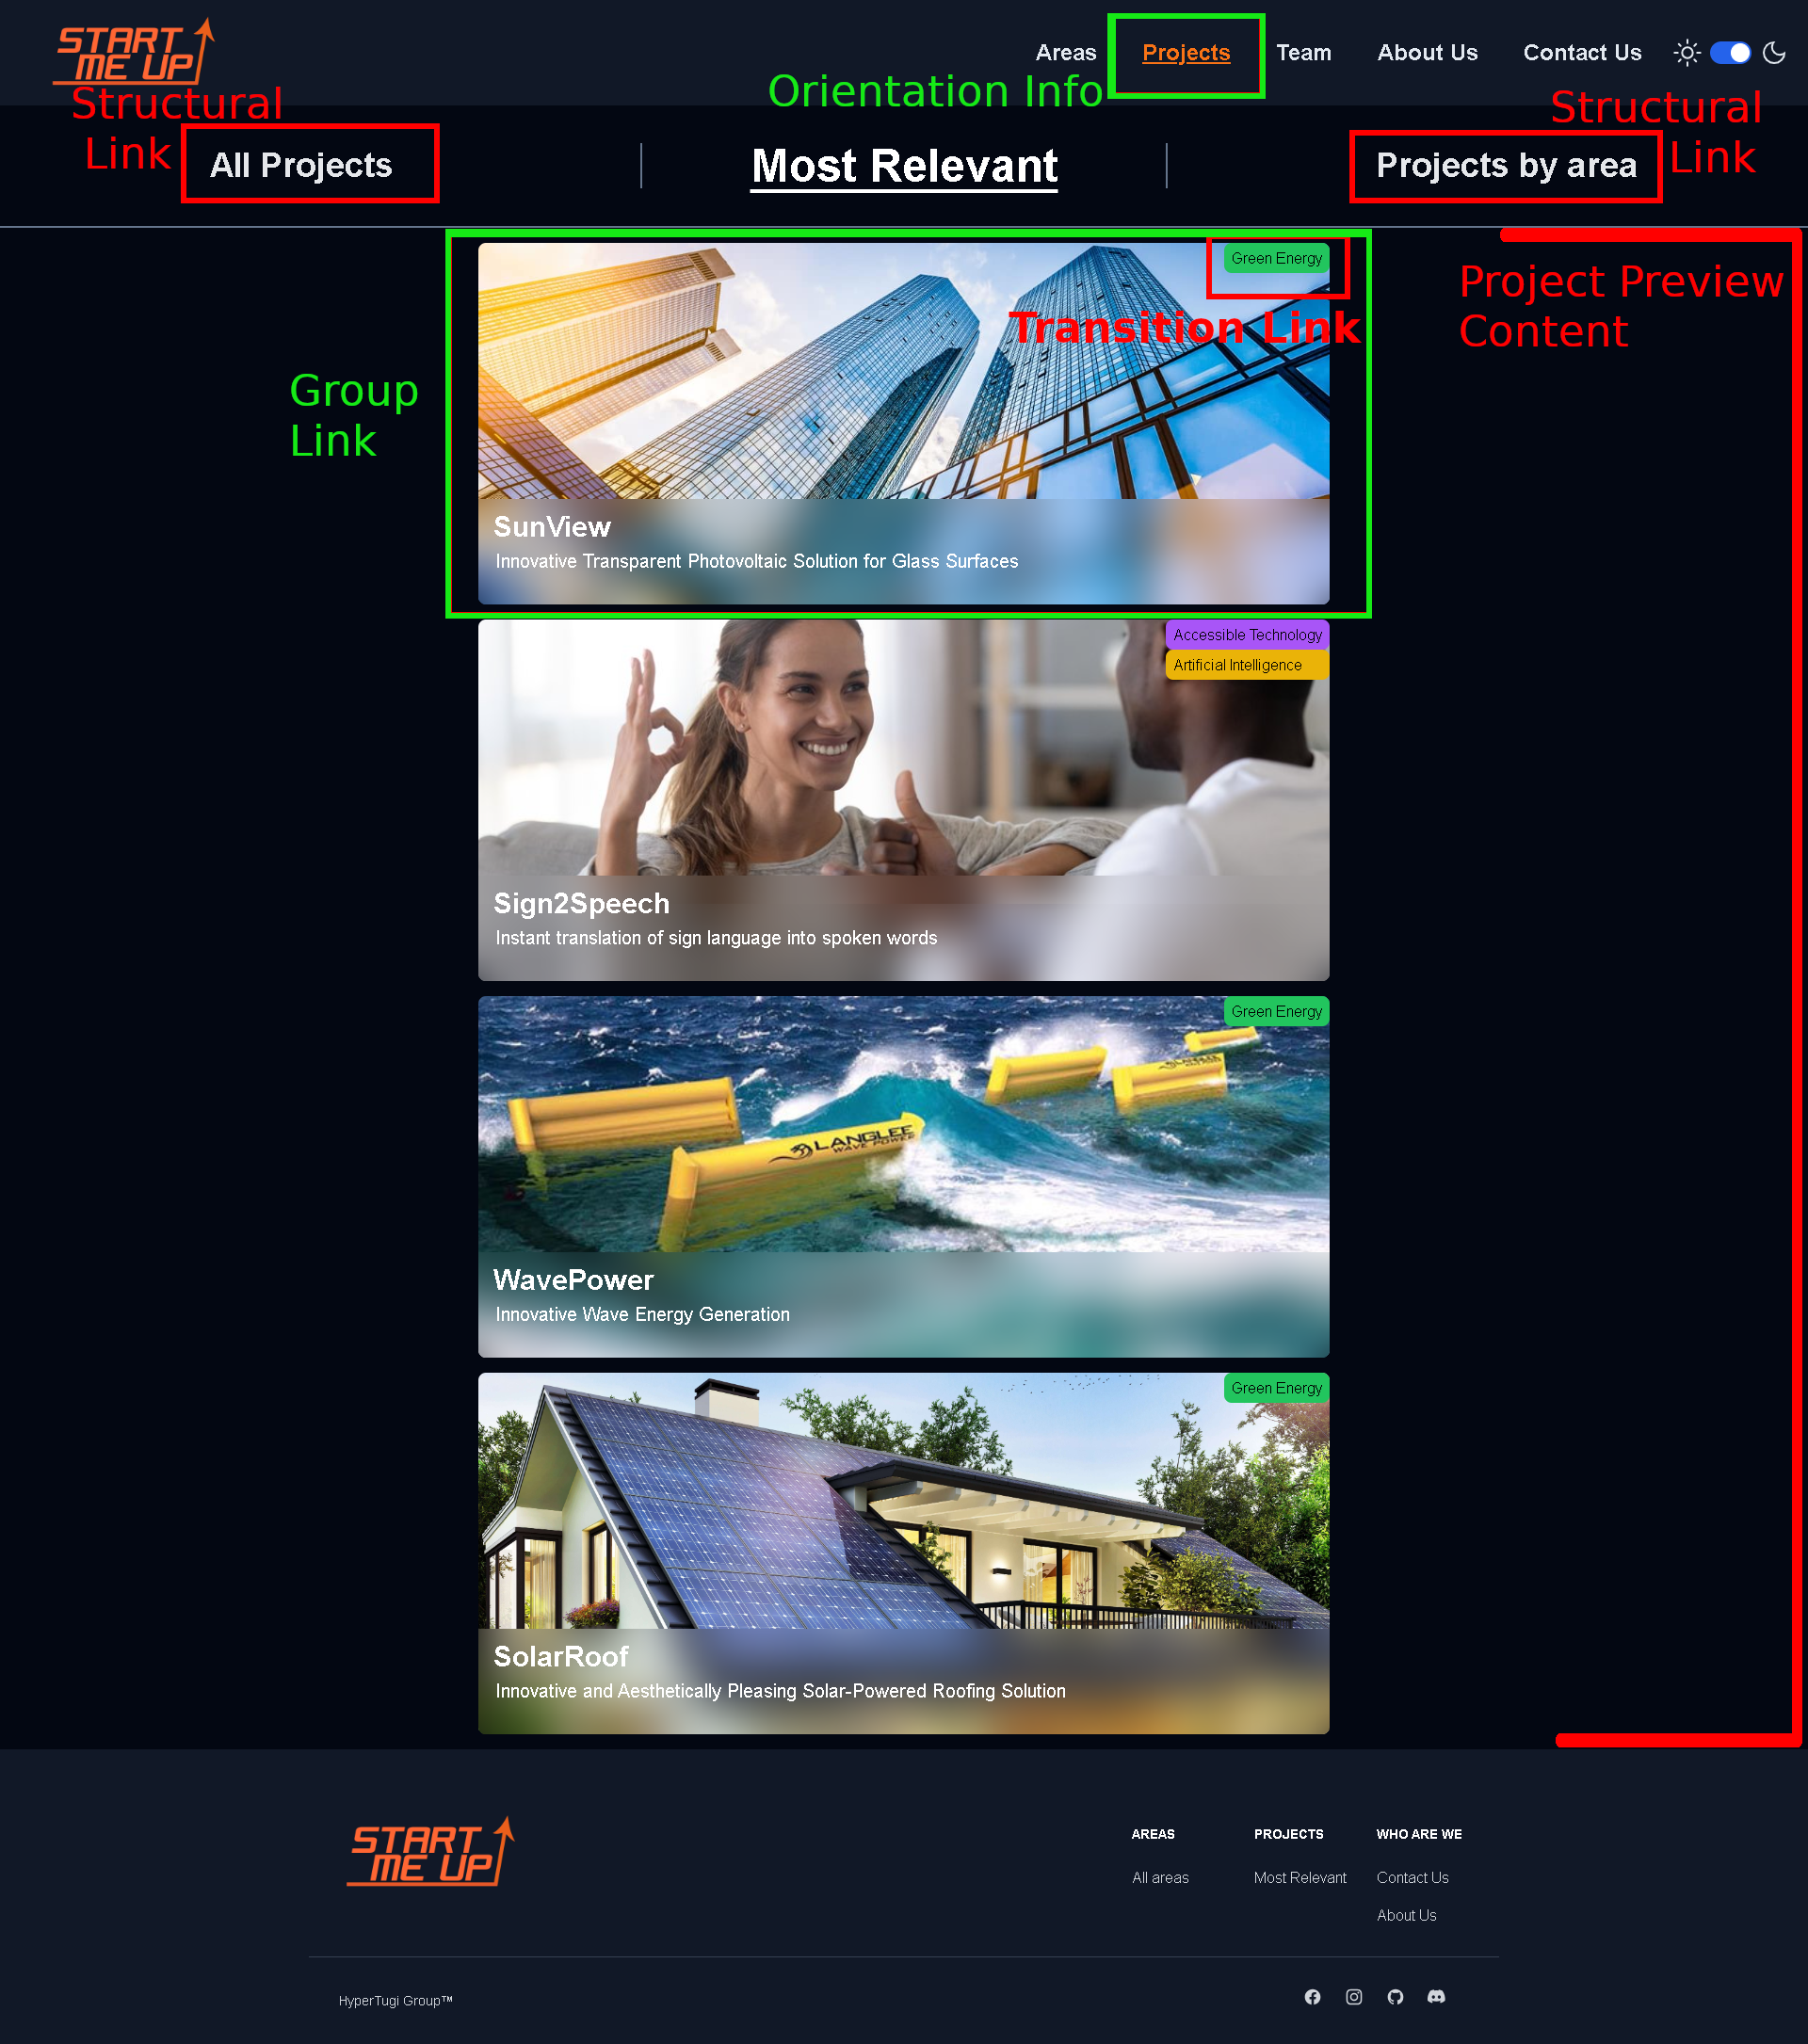
\includegraphics[width=16cm]{images/Pages Screenshots/Most Relevant Projects.png}}
    \caption{Most relevant projects - High-fidelity screenshot}
    \label{fig:PageScreenshot_Most_relevant_projects}
\end{figure}

\subsubsection*{All projects}
\begin{figure}[H]
    \centering
    \setlength{\fboxsep}{0pt}\fbox{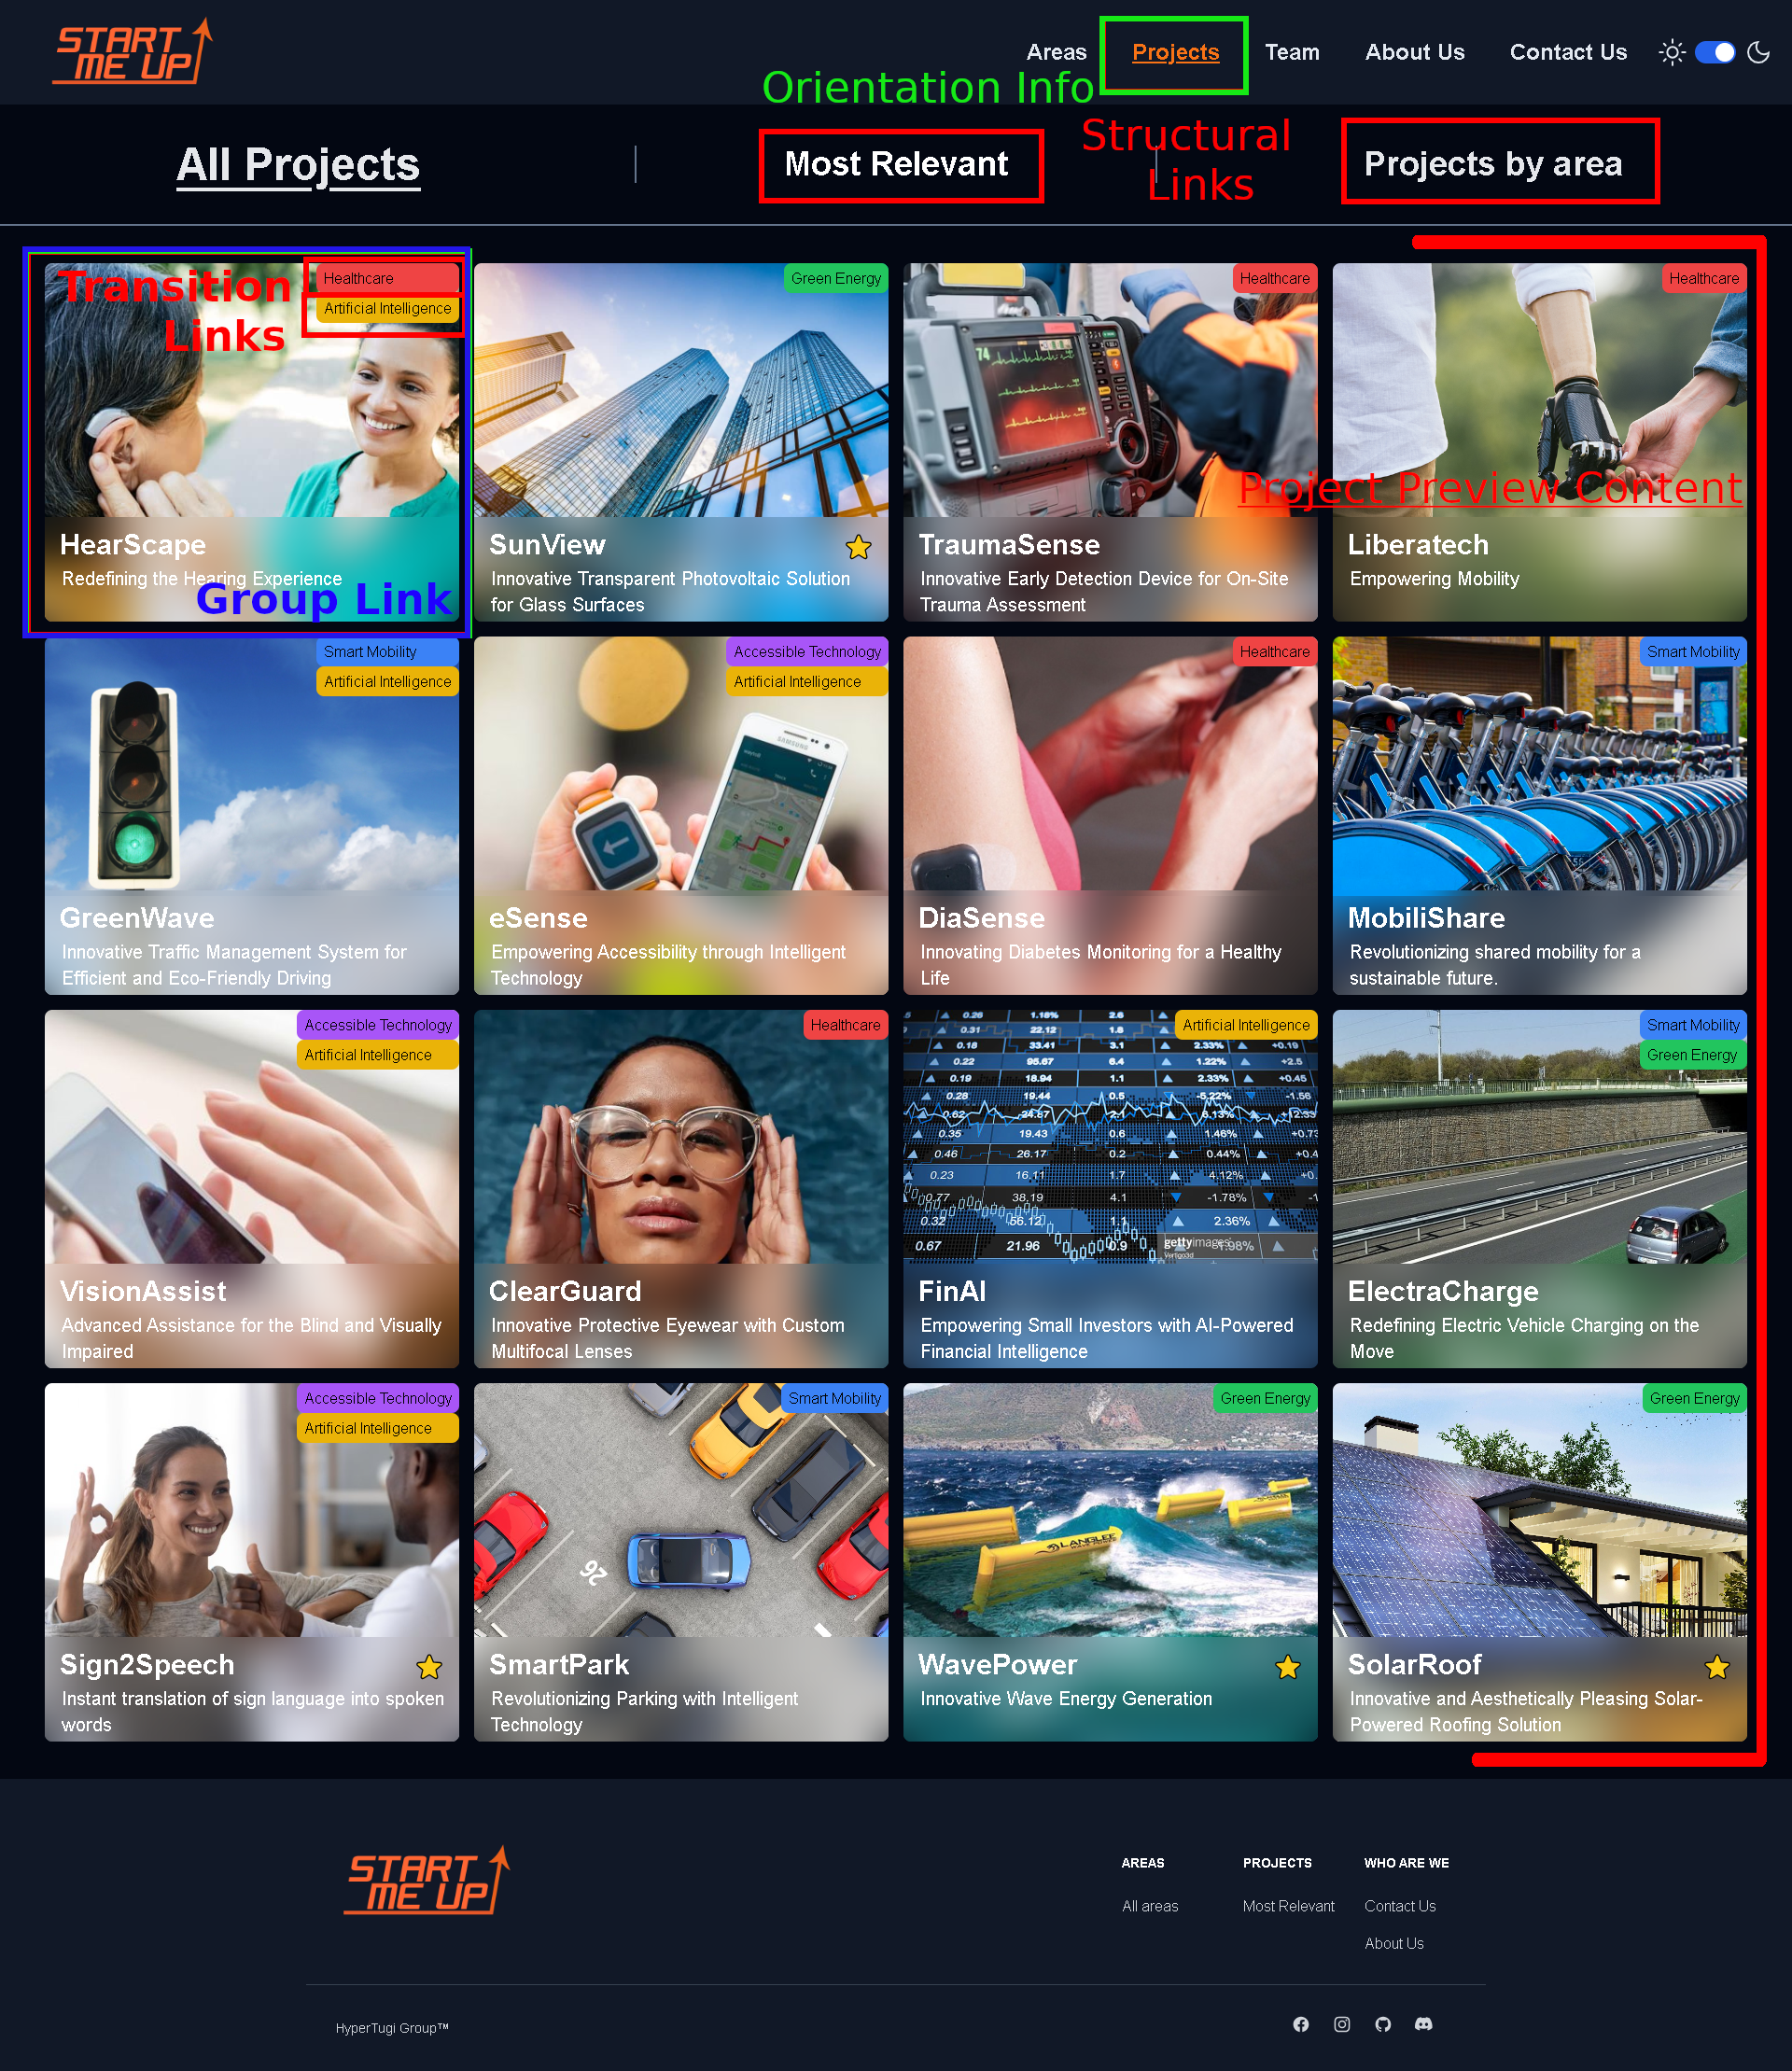
\includegraphics[width=16cm]{images/Pages Screenshots/All Projects.png}}
    \caption{All projects - High-fidelity screenshot}
    \label{fig:PageScreenshot_All_projects}
\end{figure}

\subsubsection*{Projects by area}
\begin{figure}[H]
    \centering
    \setlength{\fboxsep}{0pt}\fbox{\includegraphics[width=12cm]{images/Pages Screenshots/Projects By Area.png}}
    \caption{Projects by area - High-fidelity screenshot}
    \label{fig:PageScreenshot_Projects_by_area}
\end{figure}

\subsection{About Us}

\subsubsection*{About Us}
\begin{figure}[H]
    \centering
    \setlength{\fboxsep}{0pt}\fbox{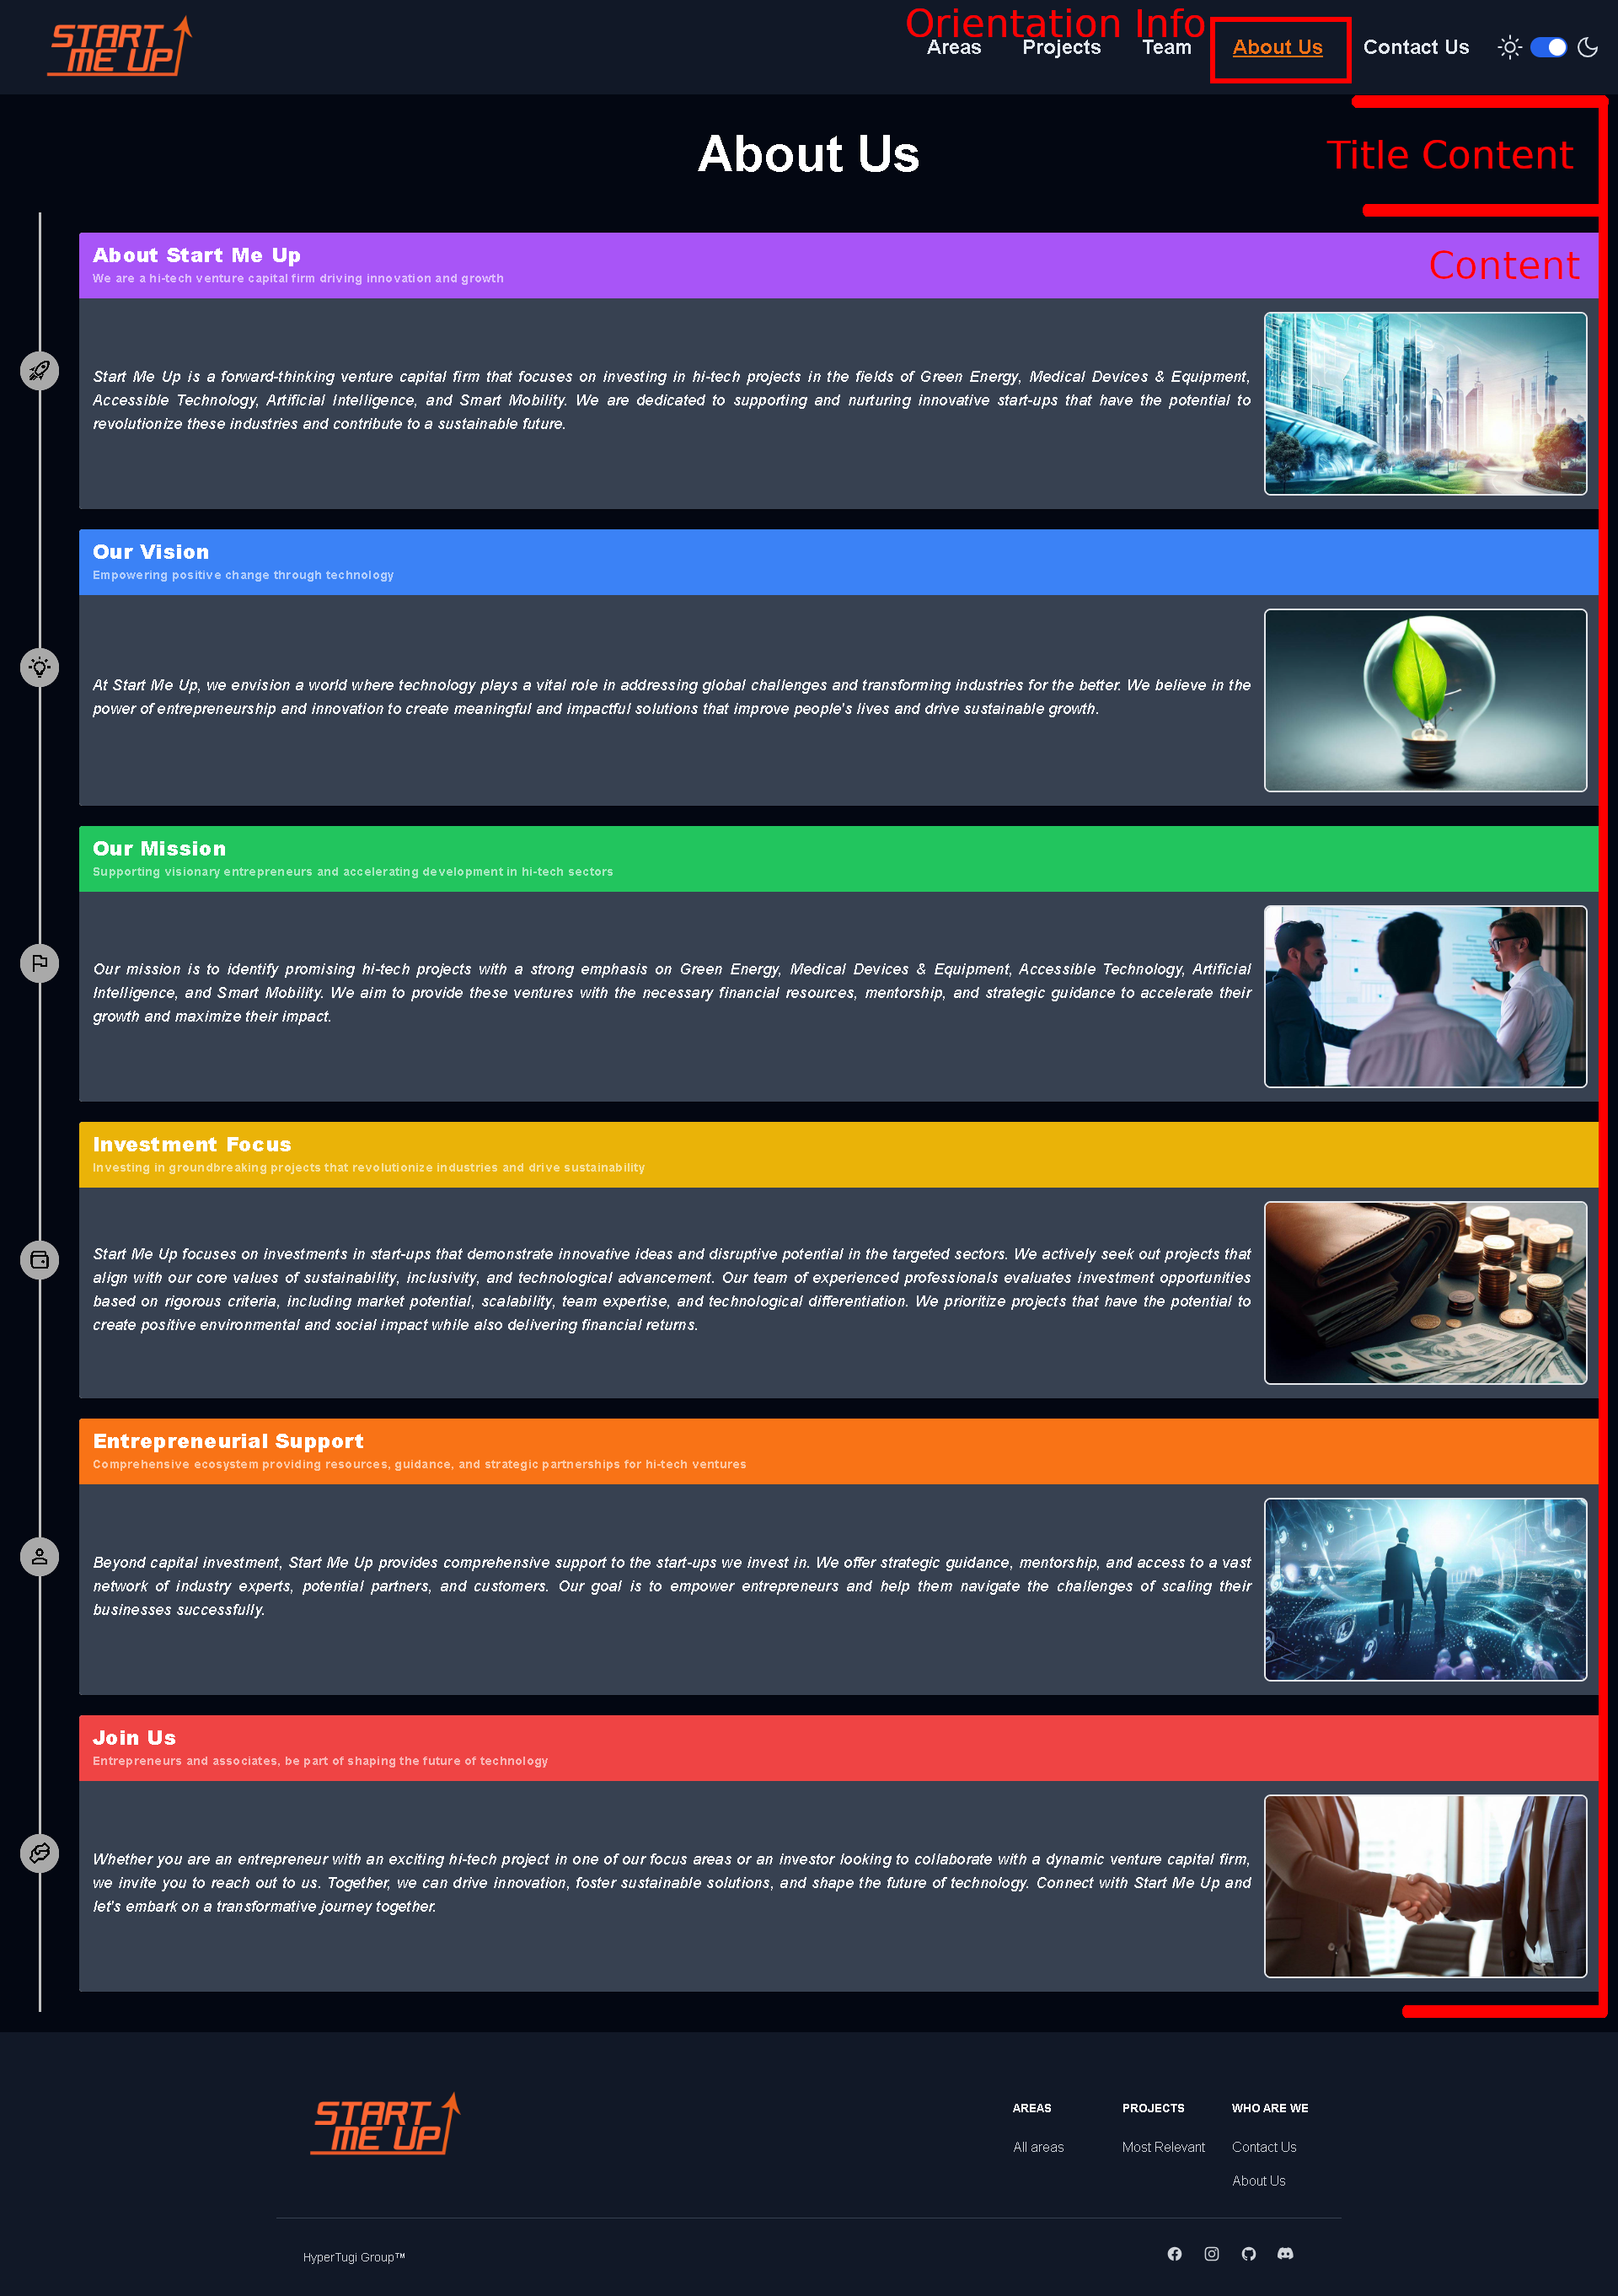
\includegraphics[width=14cm]{images/Pages Screenshots/About Us.png}}
    \caption{About Us - High-fidelity screenshot}
    \label{fig:PageScreenshot_About_Us}
\end{figure}

\subsection{Contact Us}

\subsubsection*{Contact Us}
\begin{figure}[H]
    \centering
    \setlength{\fboxsep}{0pt}\fbox{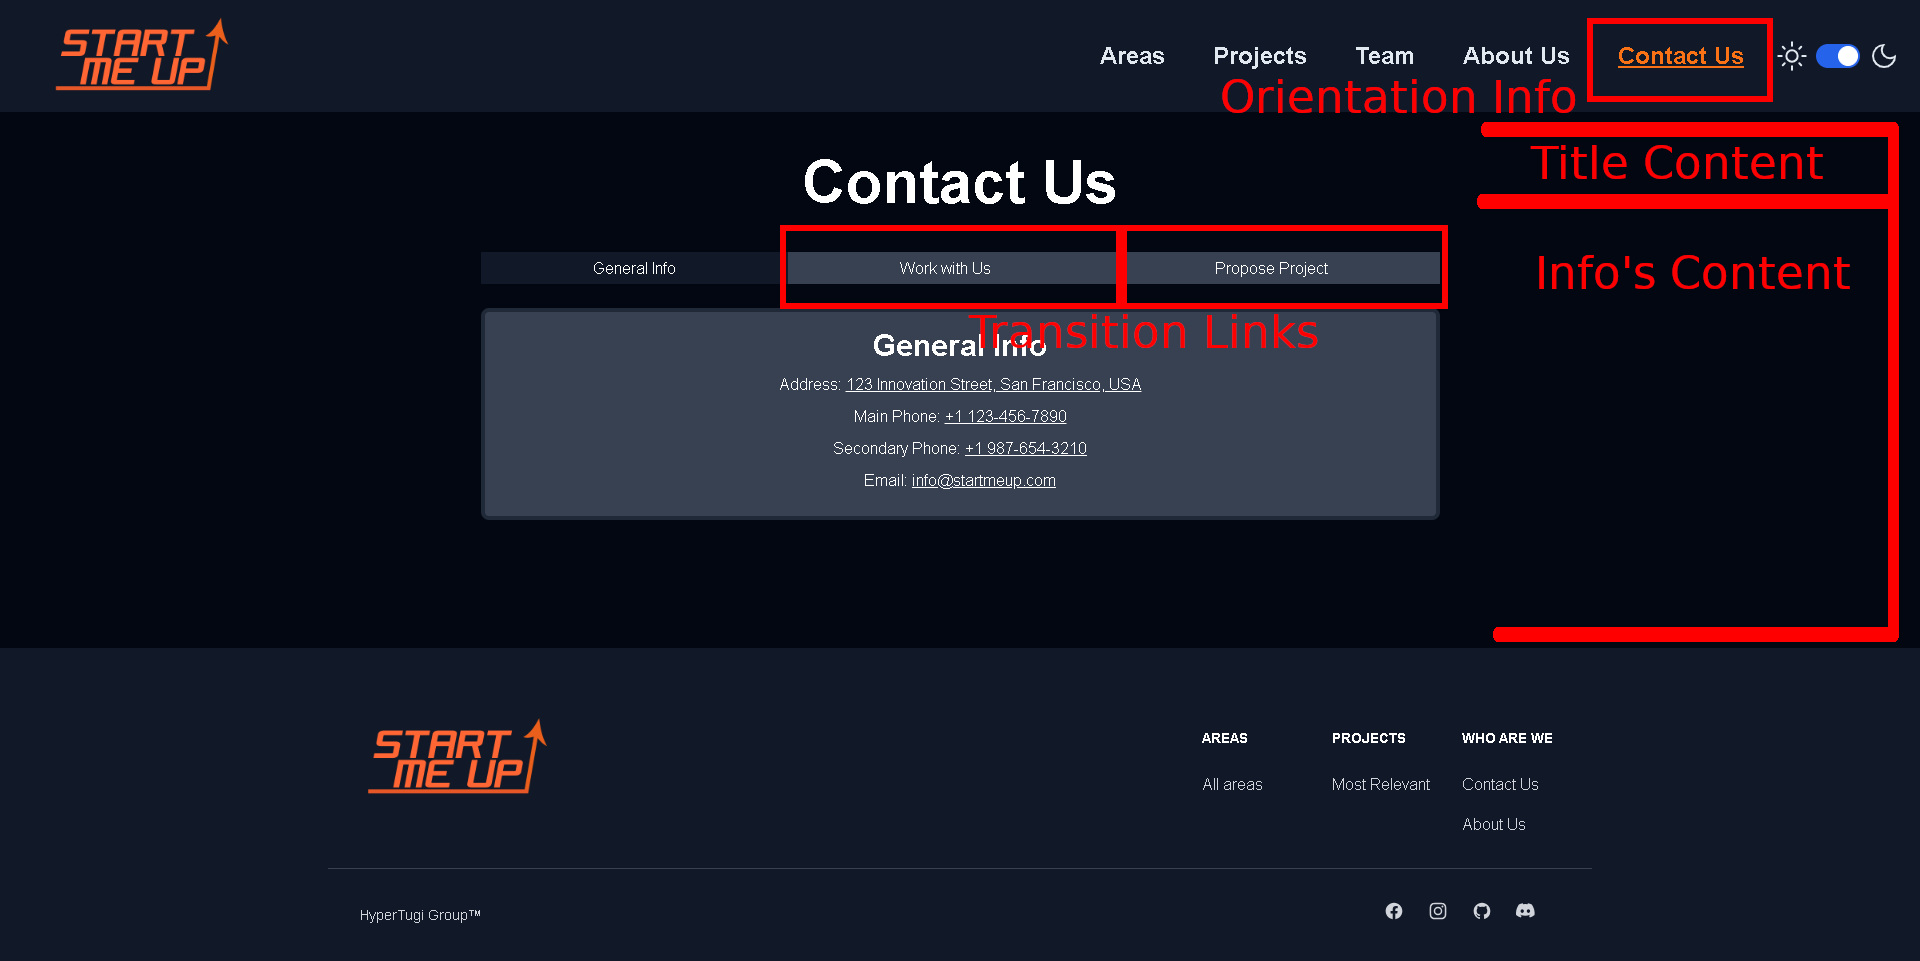
\includegraphics[width=14cm]{images/Pages Screenshots/Contact Us.png}}
    \caption{Contact Us - High-fidelity screenshot}
    \label{fig:PageScreenshot_Contact_Us}
\end{figure}

\subsubsection*{Work with Us}
\begin{figure}[H]
    \centering
    \setlength{\fboxsep}{0pt}\fbox{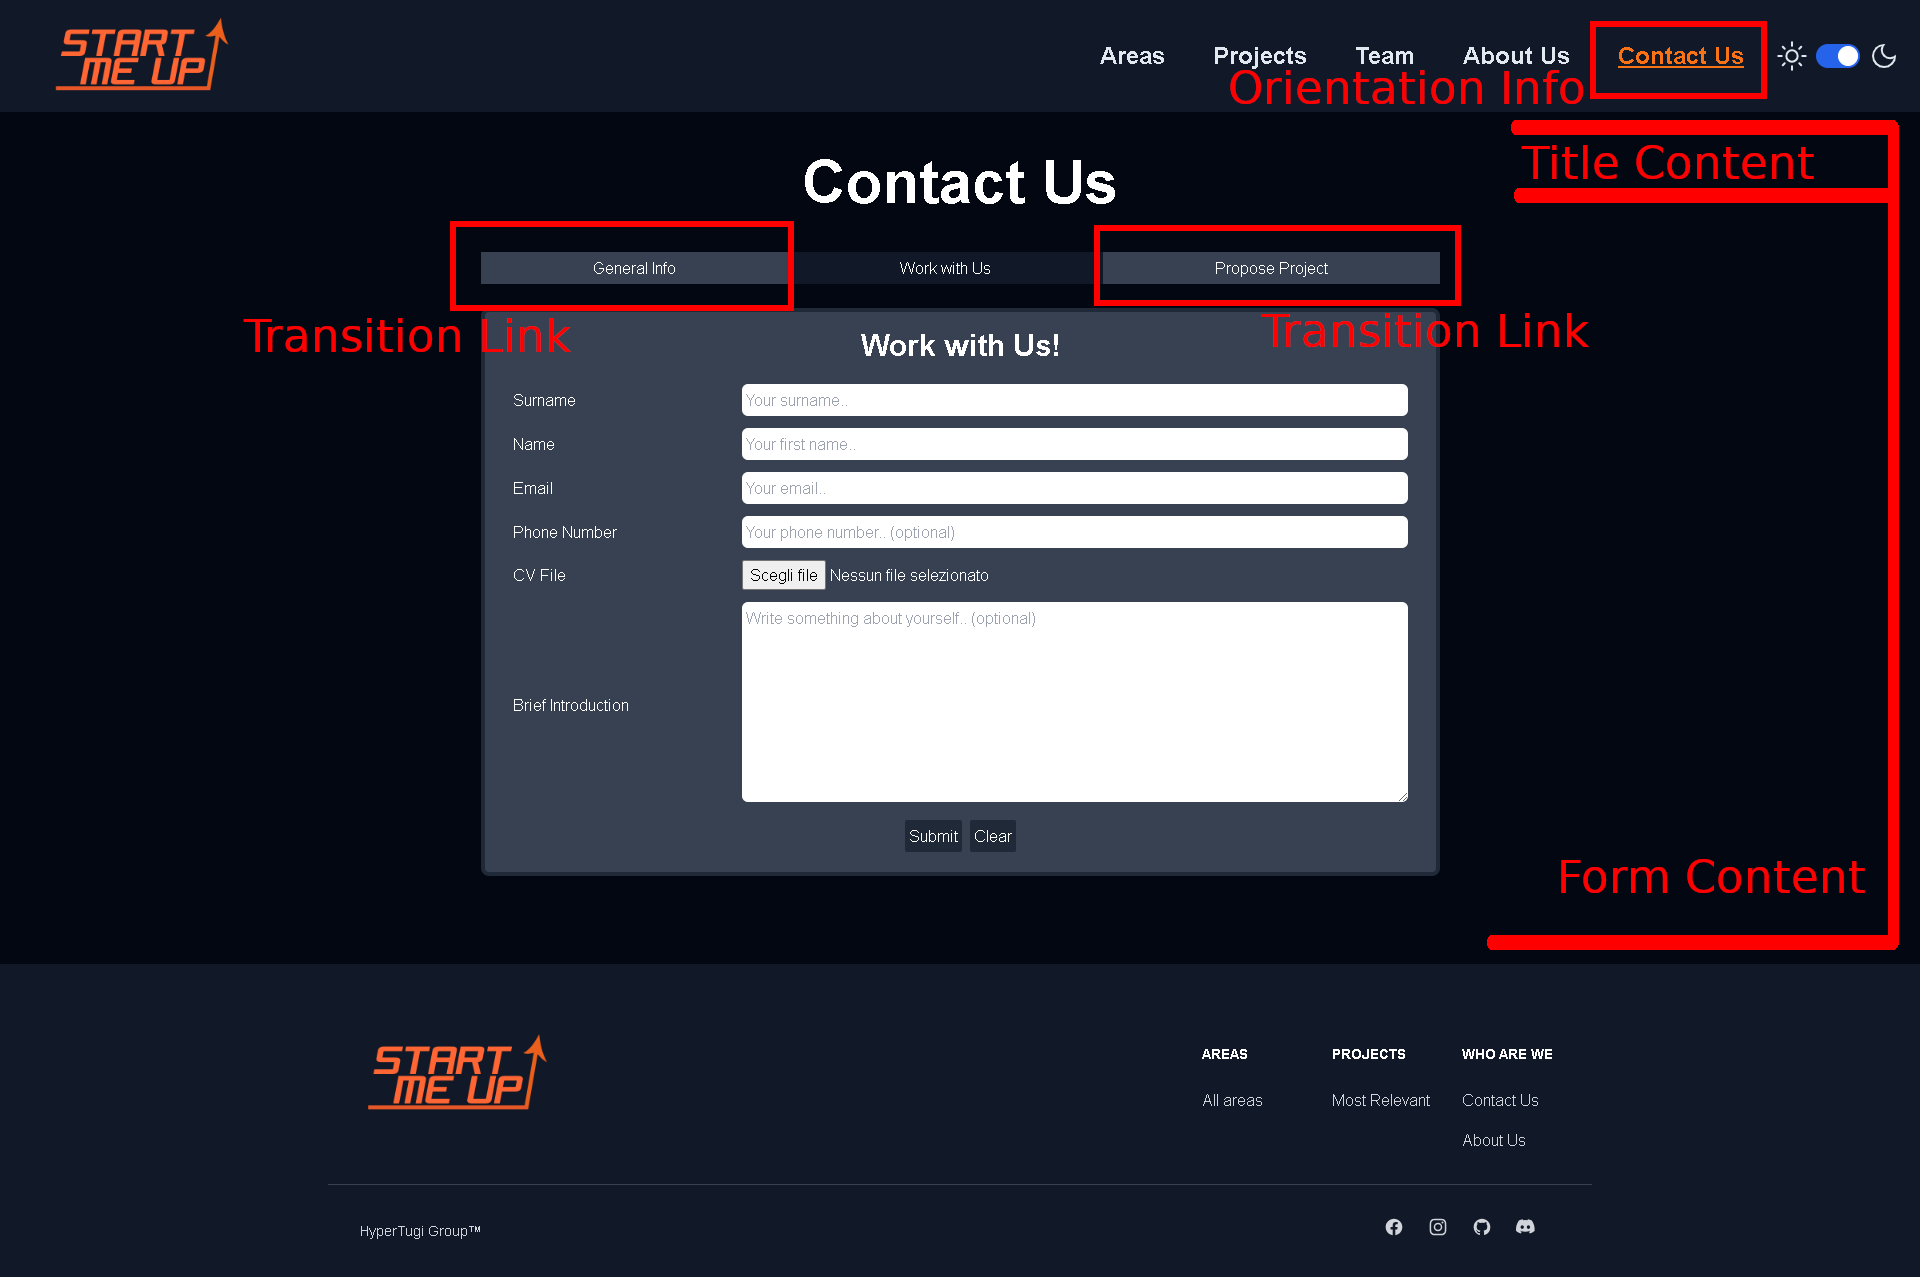
\includegraphics[width=14cm]{images/Pages Screenshots/Work With Us.png}}
    \caption{Work with Us - High-fidelity screenshot}
    \label{fig:PageScreenshot_Work_with_Us}
\end{figure}

\subsubsection*{Propose Project}
\begin{figure}[H]
    \centering
    \setlength{\fboxsep}{0pt}\fbox{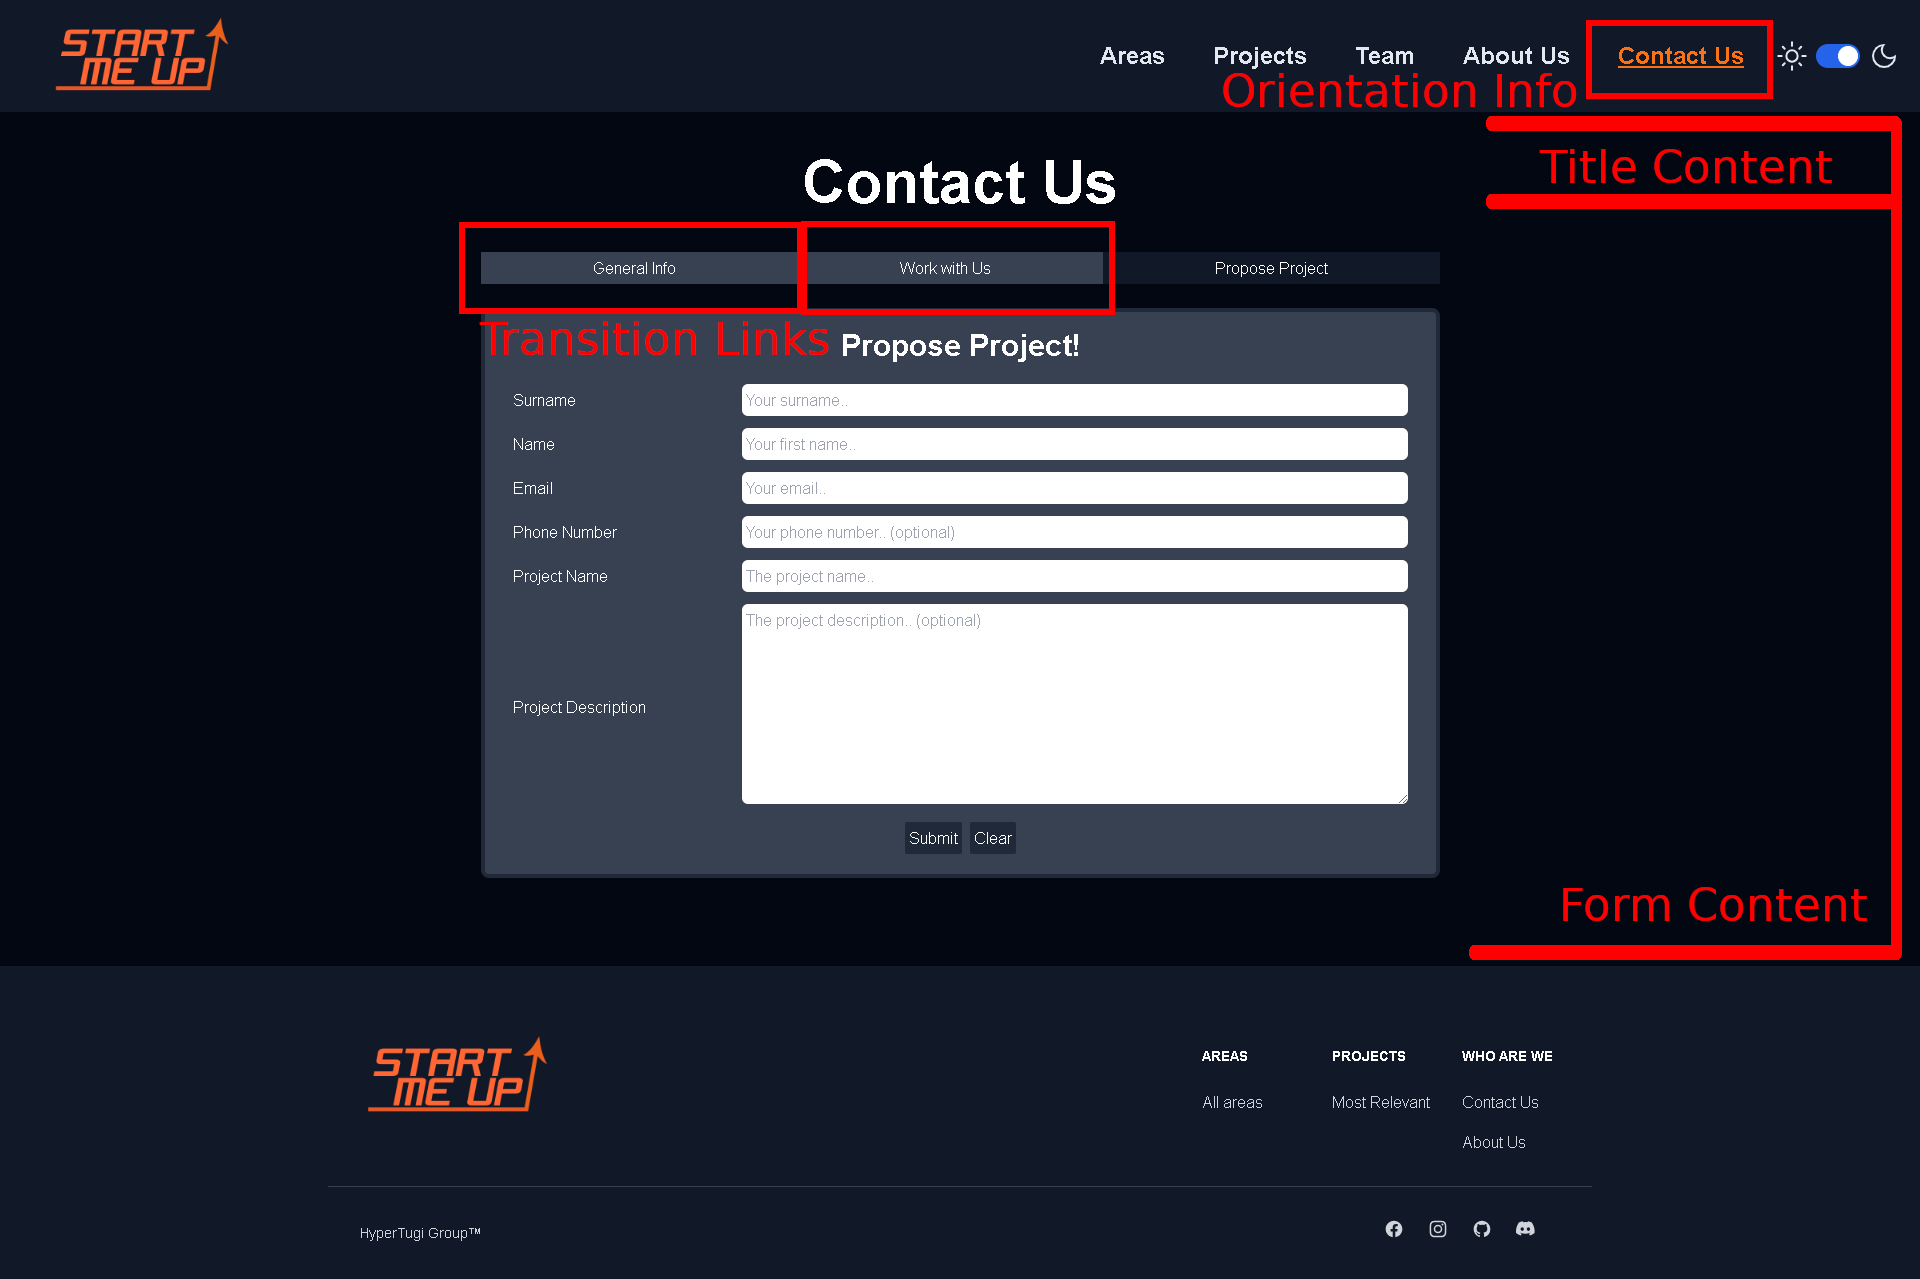
\includegraphics[width=14cm]{images/Pages Screenshots/Propose Project.png}}
    \caption{Propose Project - High-fidelity screenshot}
    \label{fig:PageScreenshot_Propose_Project}
\end{figure}

\subsubsection*{Error}
\begin{figure}[H]
    \centering
    \setlength{\fboxsep}{0pt}\fbox{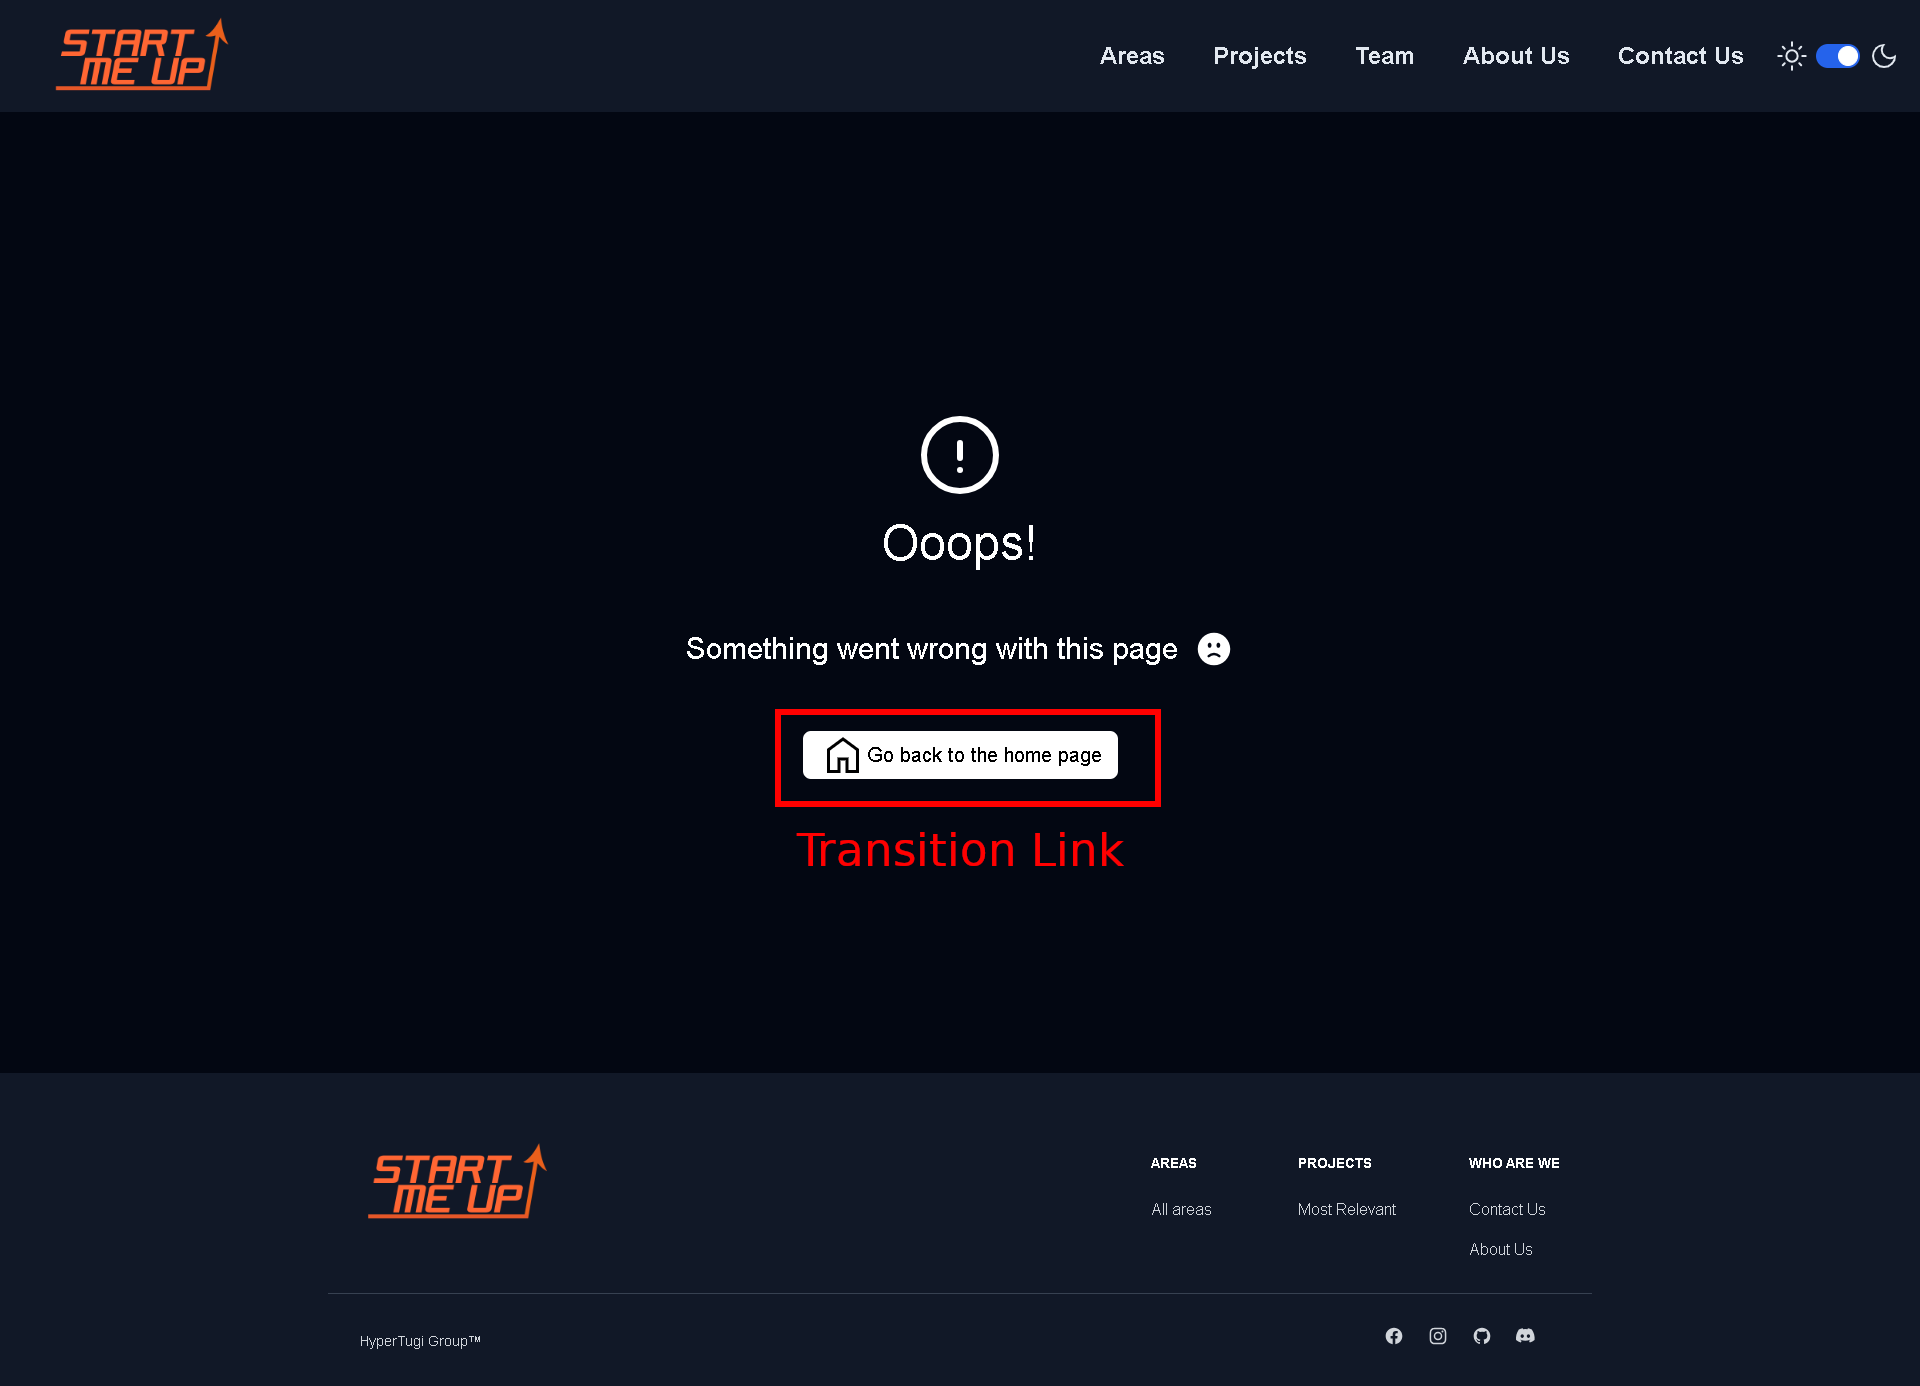
\includegraphics[width=14cm]{images/Pages Screenshots/Error.png}}
    \caption{Error page - High-fidelity screenshot}
    \label{fig:PageScreenshot_Propose_Project}
\end{figure}

\clearpage

\section{Interaction Scenarios}
\subsection{Scenario 1}
Lorenzo is an entrepreneur with an innovative idea for a green energy start-up. He needs funding to kickstart his company and has heard great things about a venture capital firm called "StartMeUp” He decides to visit the company's website with a computer to find out what kind of projects they have funded in the past that have become successful.
\begin{figure}[H]
    \centering
    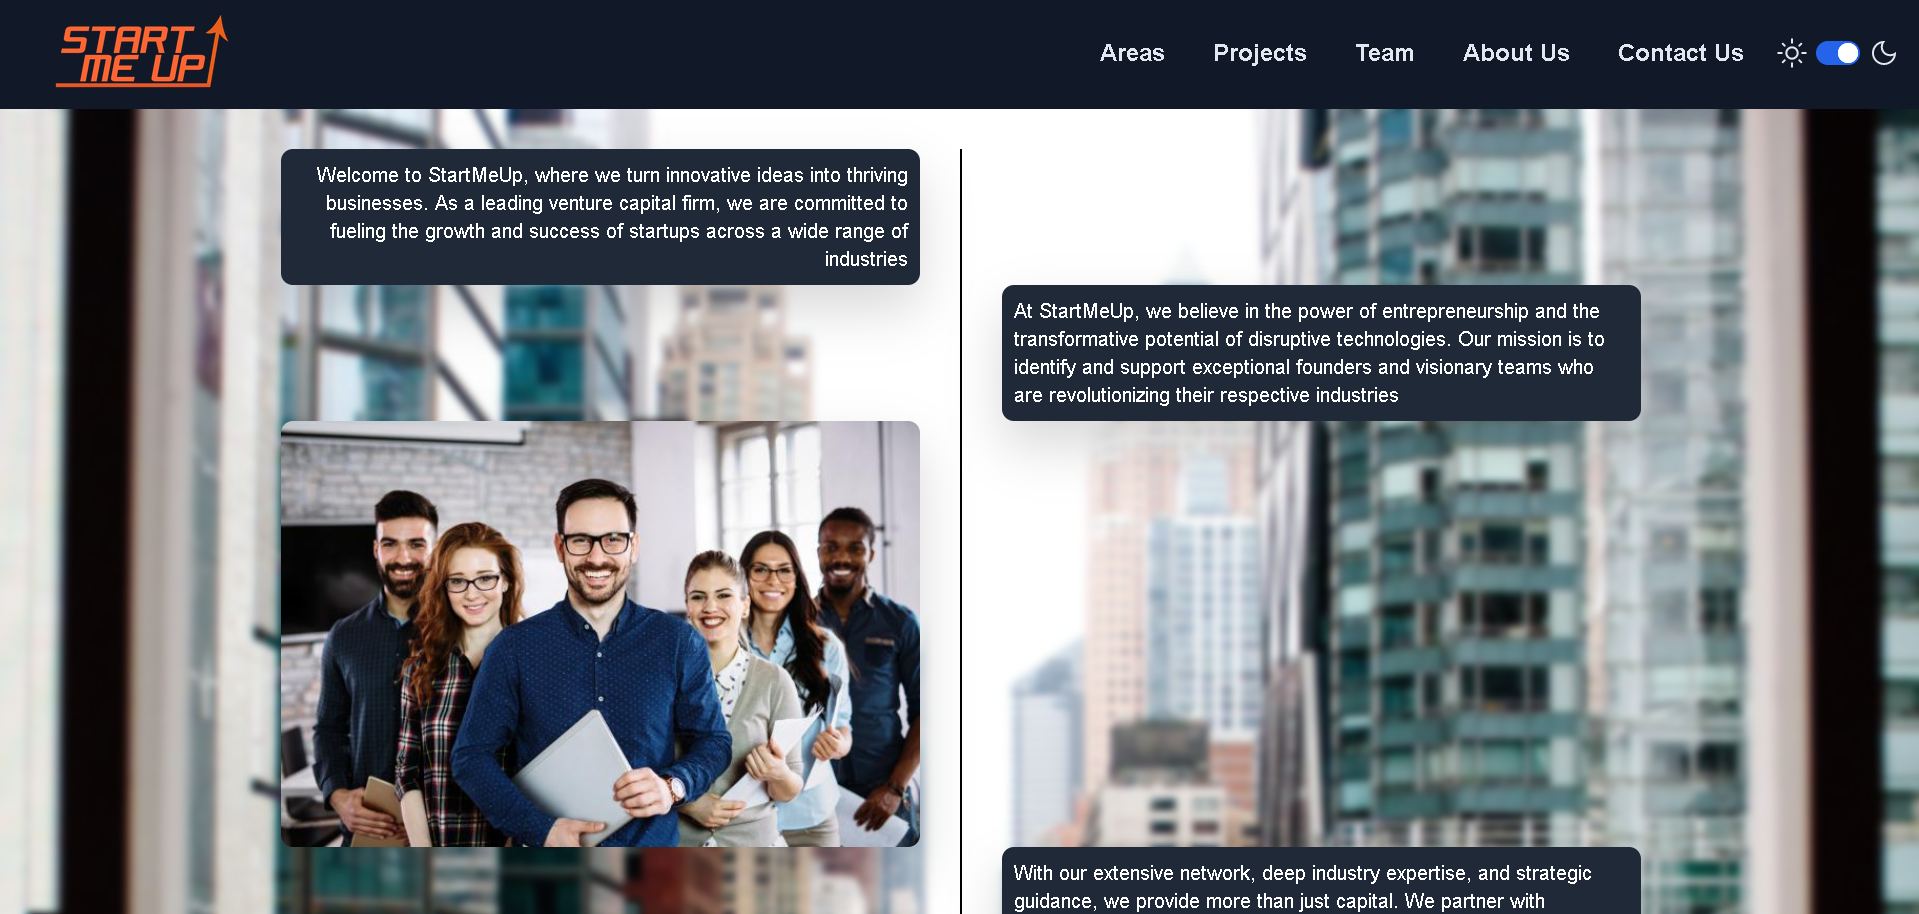
\includegraphics[width=16cm]{images/Scenarios/Scenario 1/Screen1.png}
    \caption{Homepage}
    \label{fig:scenario1_1}
\end{figure}
\noindent
Lorenzo navigates to the homepage of the website and clicks on the "Projects" section from the menu to conduct his research. 
\begin{figure}[H]
    \centering
    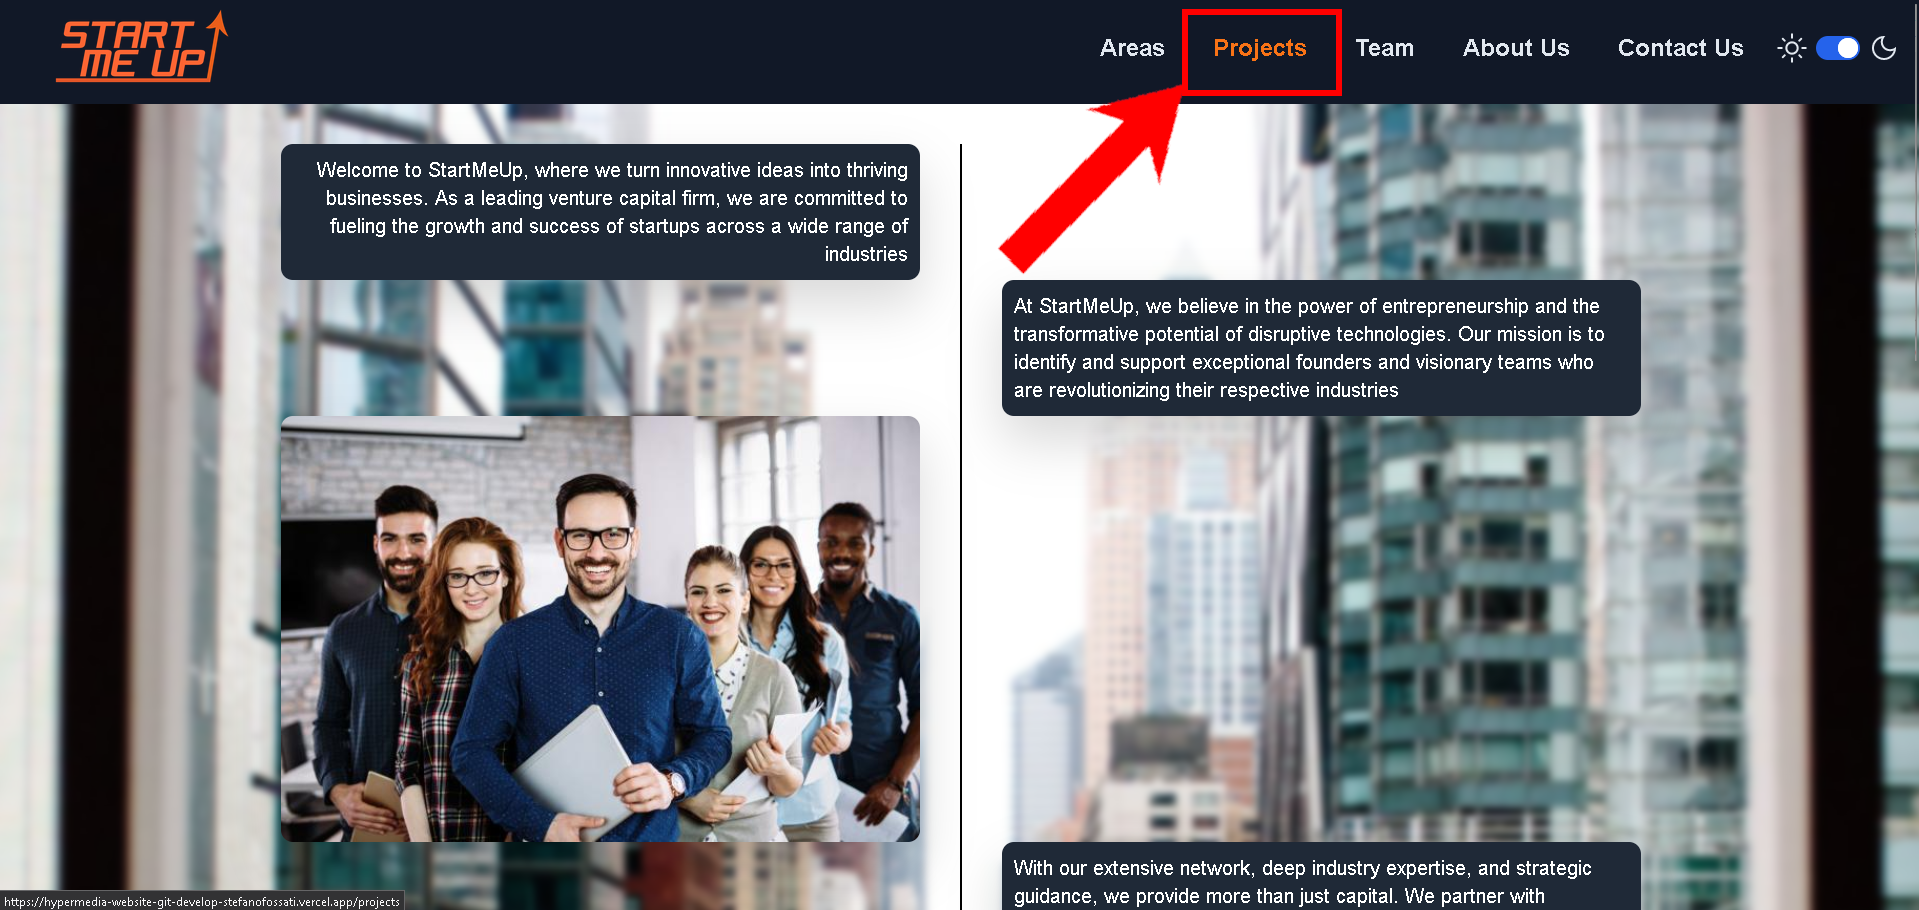
\includegraphics[width=16cm]{images/Scenarios/Scenario 1/Screen2.png}
    \caption{Click on "Projects"}
    \label{fig:scenario1_2}
\end{figure} 
\noindent
On this page, he is particularly interested in exploring older projects within the same domain as his company. He clicks on "Projects by Area" and selects the relevant category, focusing on green energy projects.
\begin{figure}[H]
    \centering
    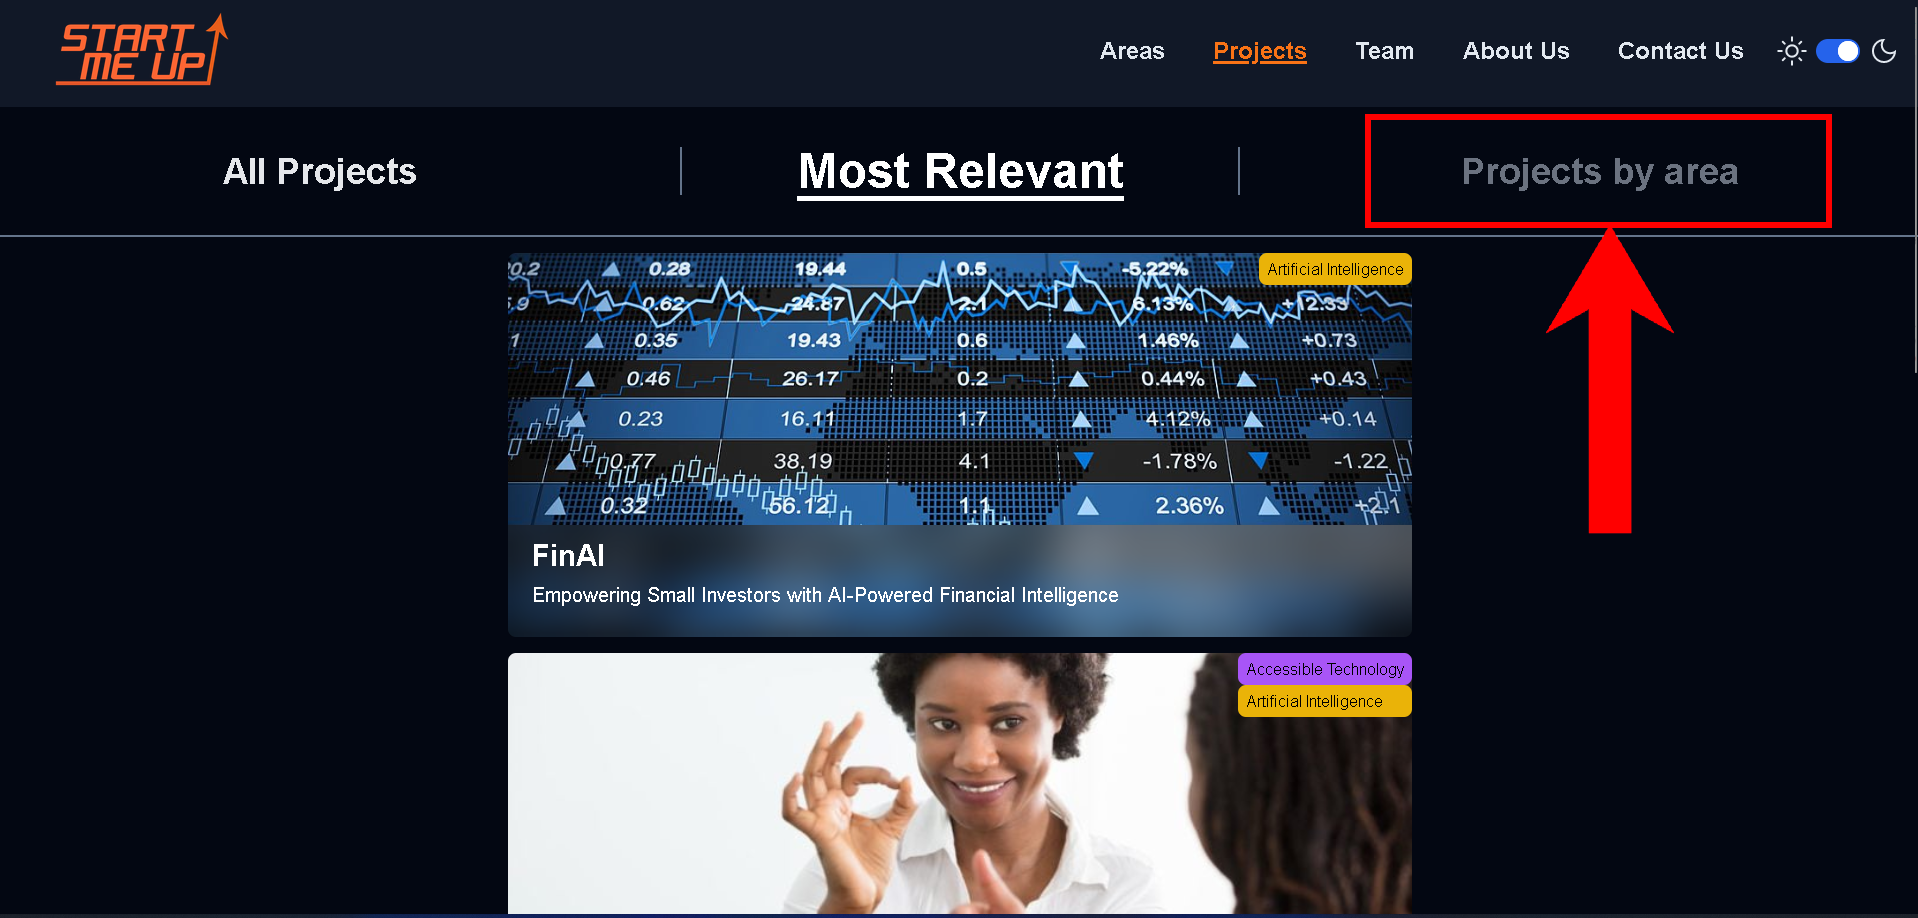
\includegraphics[width=16cm]{images/Scenarios/Scenario 1/Screen3.png}
    \caption{Click on "Projects by area"}
    \label{fig:scenario1_3}
\end{figure}
\noindent
He views the project preview and clicks on the specific area highlighted in green.
\begin{figure}[H]
    \centering
    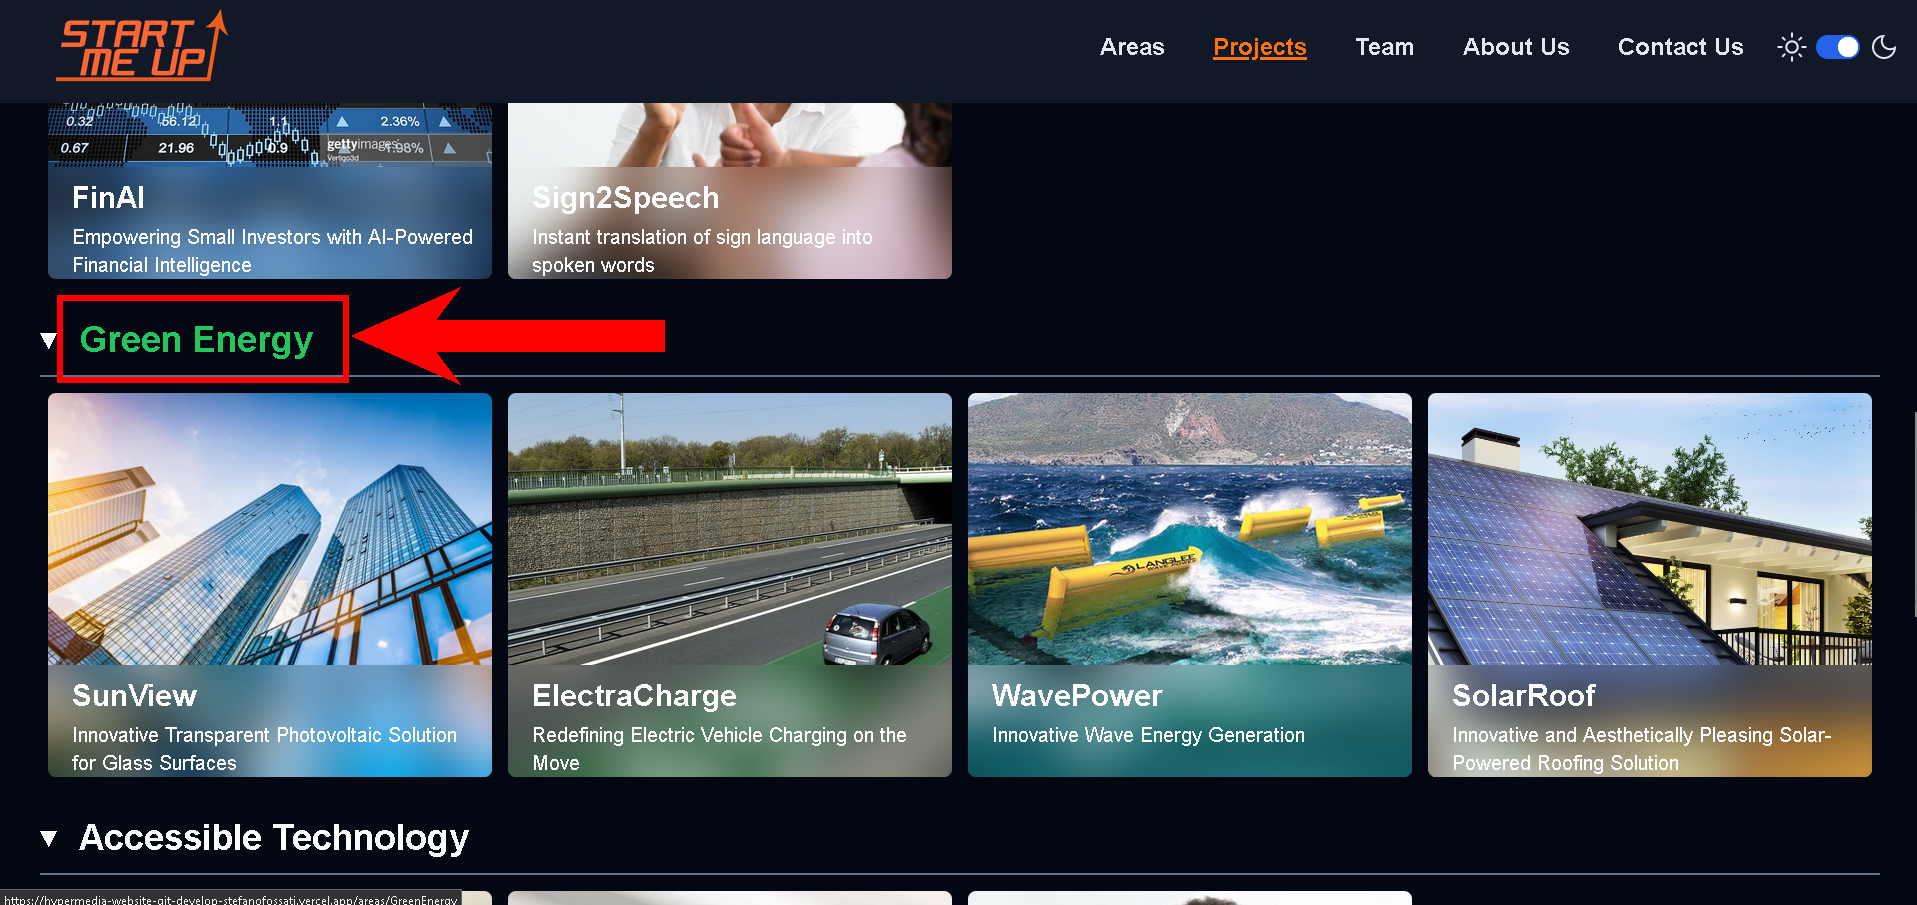
\includegraphics[width=16cm]{images/Scenarios/Scenario 1/Screen4.png}
    \caption{Click on "Green Energy"}
    \label{fig:scenario1_4}
\end{figure}
\noindent
From there, he explores the specific area and reads the description to assess whether his project aligns with the venture capital's investment focus area.
\begin{figure}[H]
    \centering
    
\includegraphics[width=16cm]{images/Scenarios/Scenario 1/Screen5.png}
    \caption{Scroll through page}
    \label{fig:scenario1_5}
\end{figure}
\noindent
After confirming that his project fits within their investment area, Lorenzo proceeds to the "Contact Us" section.
\begin{figure}[H]
    \centering
    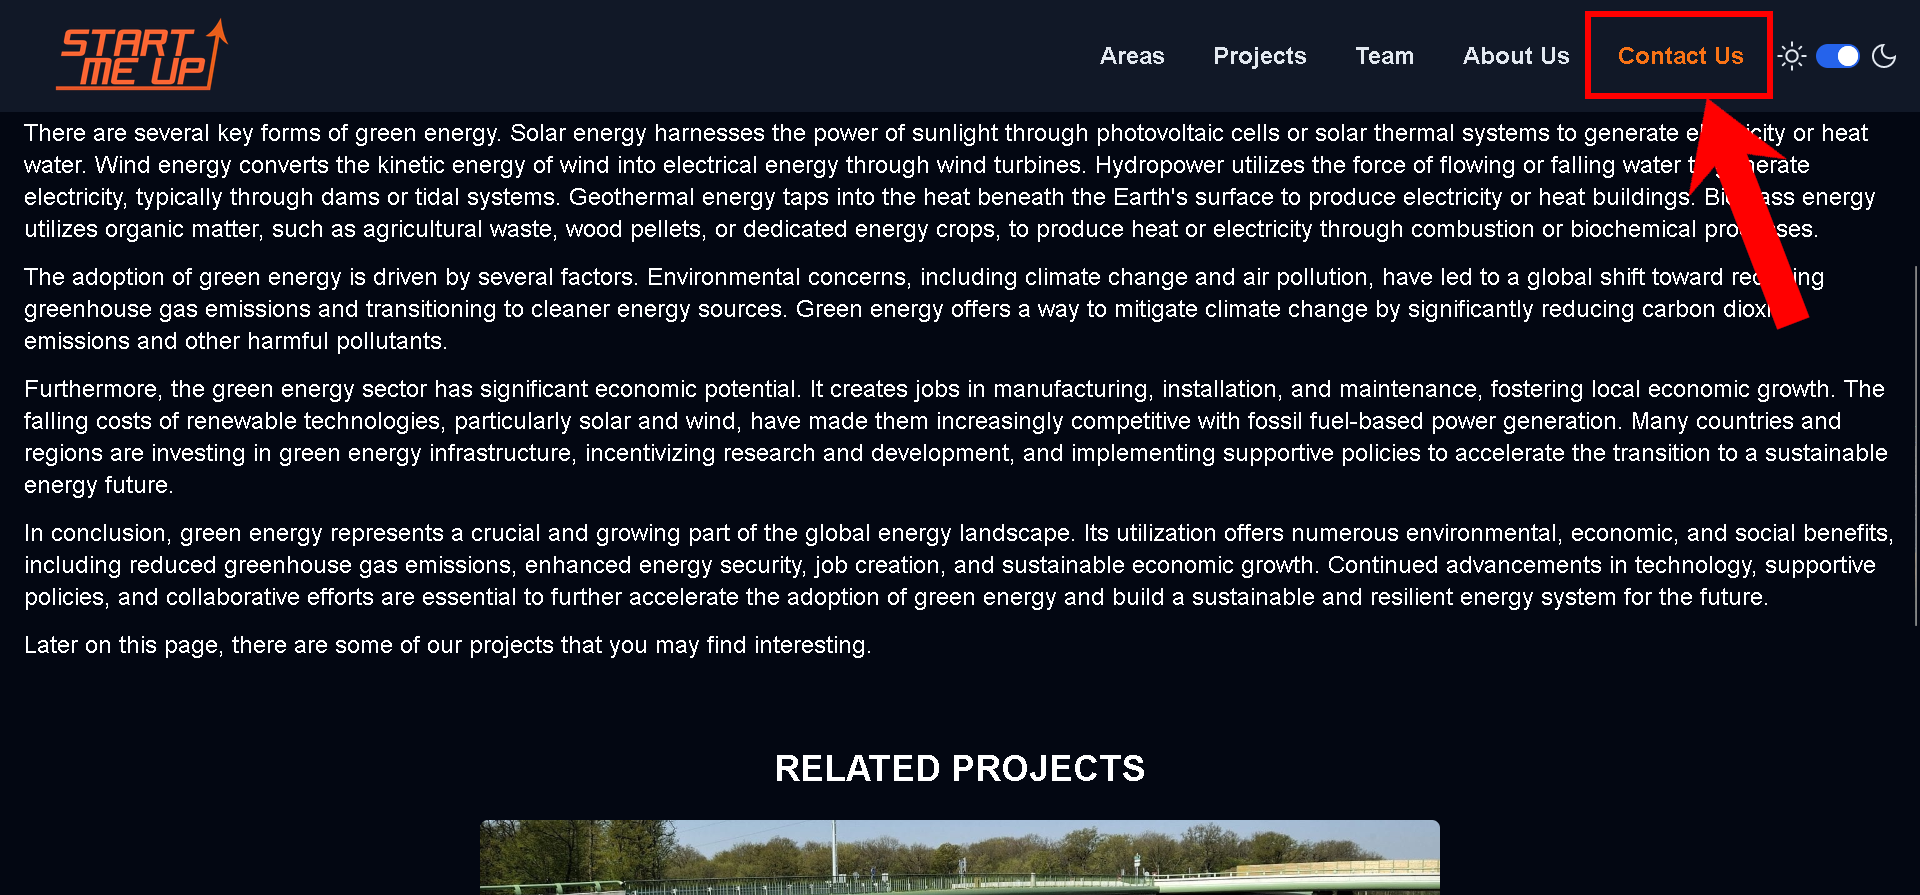
\includegraphics[width=16cm]{images/Scenarios/Scenario 1/Screen6.png}
    \caption{Click on "Contact Us"}
    \label{fig:scenario1_6}
\end{figure}
\noindent
Upon reviewing the information provided, he notices a dedicated section for proposing projects to the investors.
\begin{figure}[H]
    \centering
    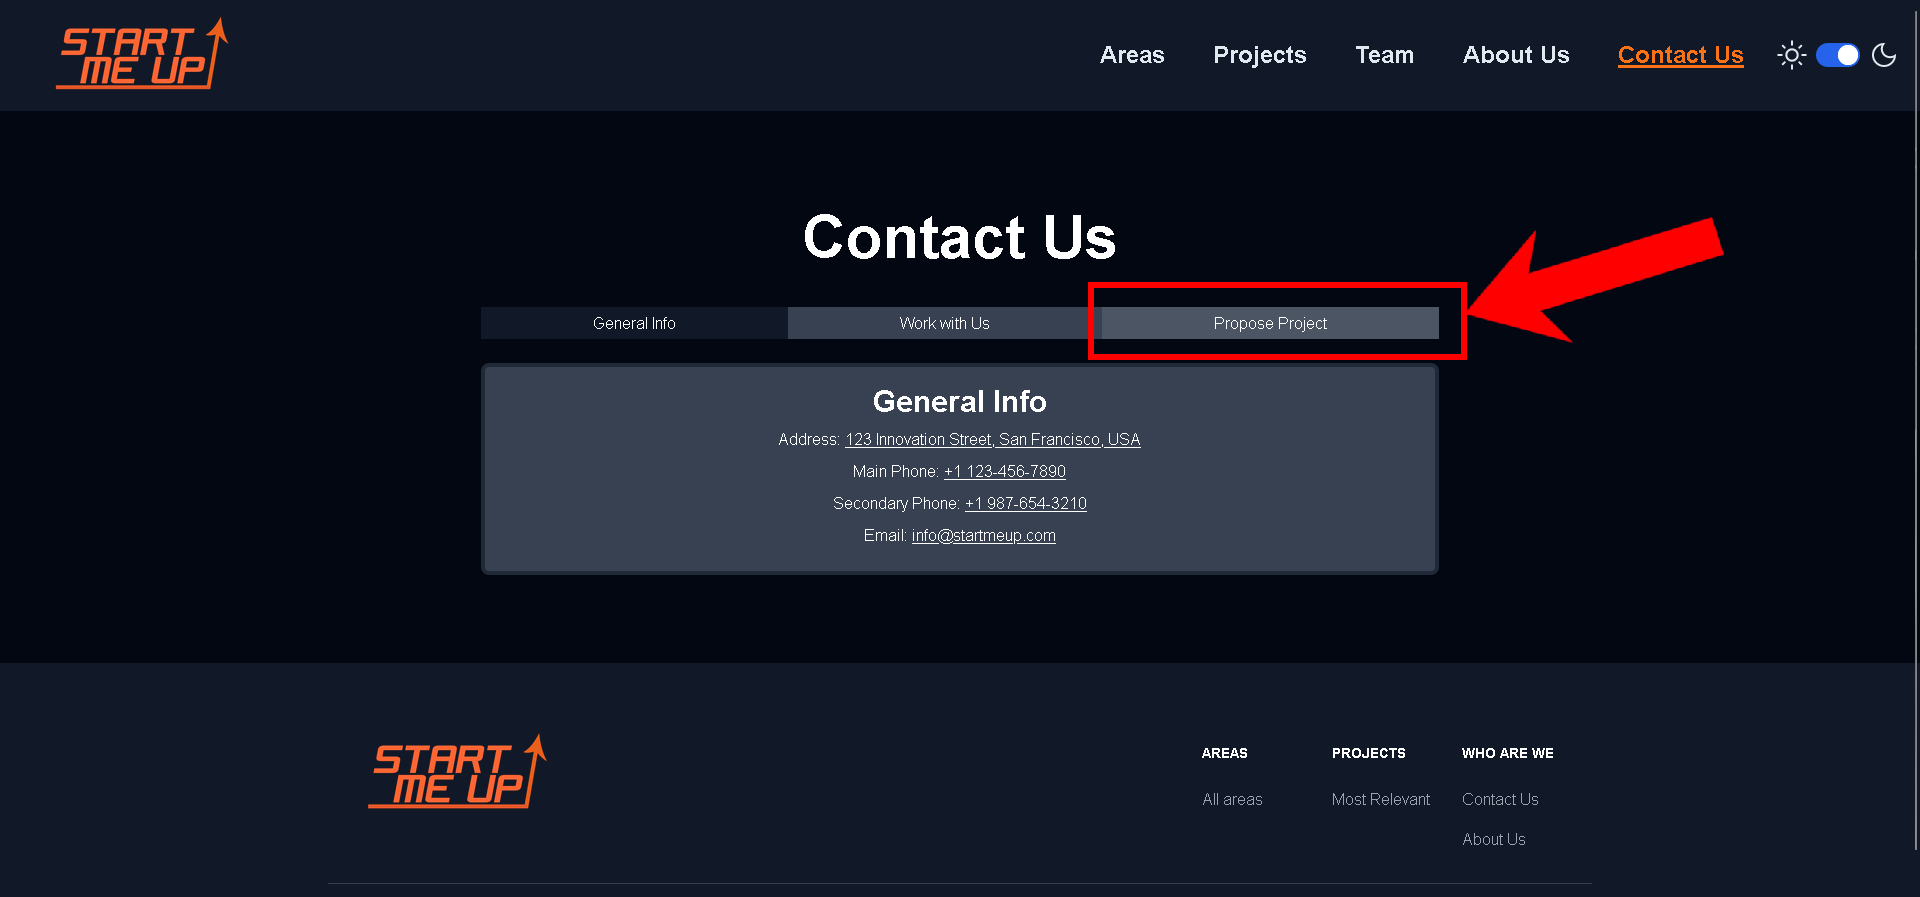
\includegraphics[width=16cm]{images/Scenarios/Scenario 1/Screen7.png}
    \caption{Click on "Propose Project"}
    \label{fig:scenario1_7}
\end{figure}
\noindent
This encourages him as he realizes there is a formal channel to present his project to the venture capitalists and decides to compile it in order to send his propose project.
\begin{figure}[H]
    \centering
    
\includegraphics[width=16cm]{images/Scenarios/Scenario 1/Screen8.png}
    \caption{Fill the form and click "Submit"}
    \label{fig:scenario1_8}
\end{figure}
\noindent
He sends the form and receives a confirmation.
\begin{figure}[H]
    \centering
    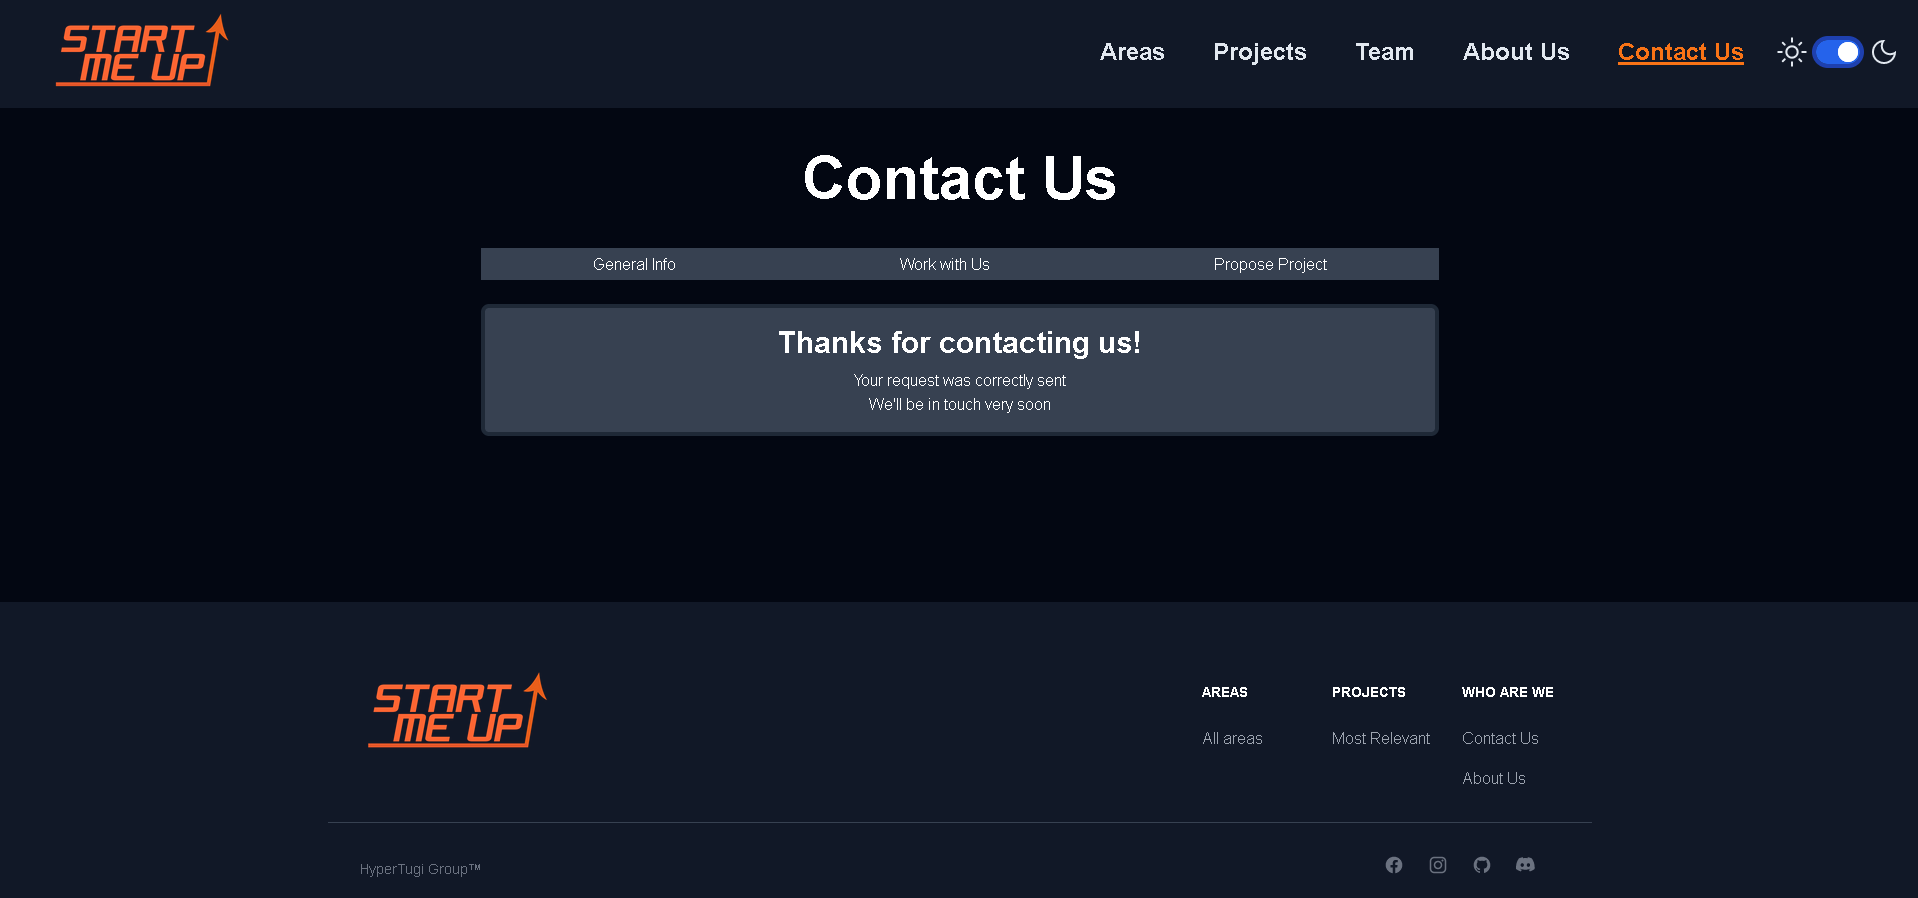
\includegraphics[width=16cm]{images/Scenarios/Scenario 1/Screen9.png}
    \caption{Form sent}
    \label{fig:scenario1_9}
\end{figure}

\subsection{Scenario 2}
Giulia is a young professional with a strong passion for technological innovation, particularly in the field of artificial intelligence, and supporting start-ups. She has heard great things about a renowned venture capital firm called " StartMeUp " and has decided that it would be an ideal place to develop her career in the field of technology investments. Giulia decides to visit the website of StartMeUp to learn more and assess if it could be a good fit for working with them.\\
Giulia accesses the website and finds a brief introduction to the venture capital, its goals, and the team on the homepage.\\

\begin{figure}[H]
    \centering
    \setlength{\fboxsep}{0pt}\fbox{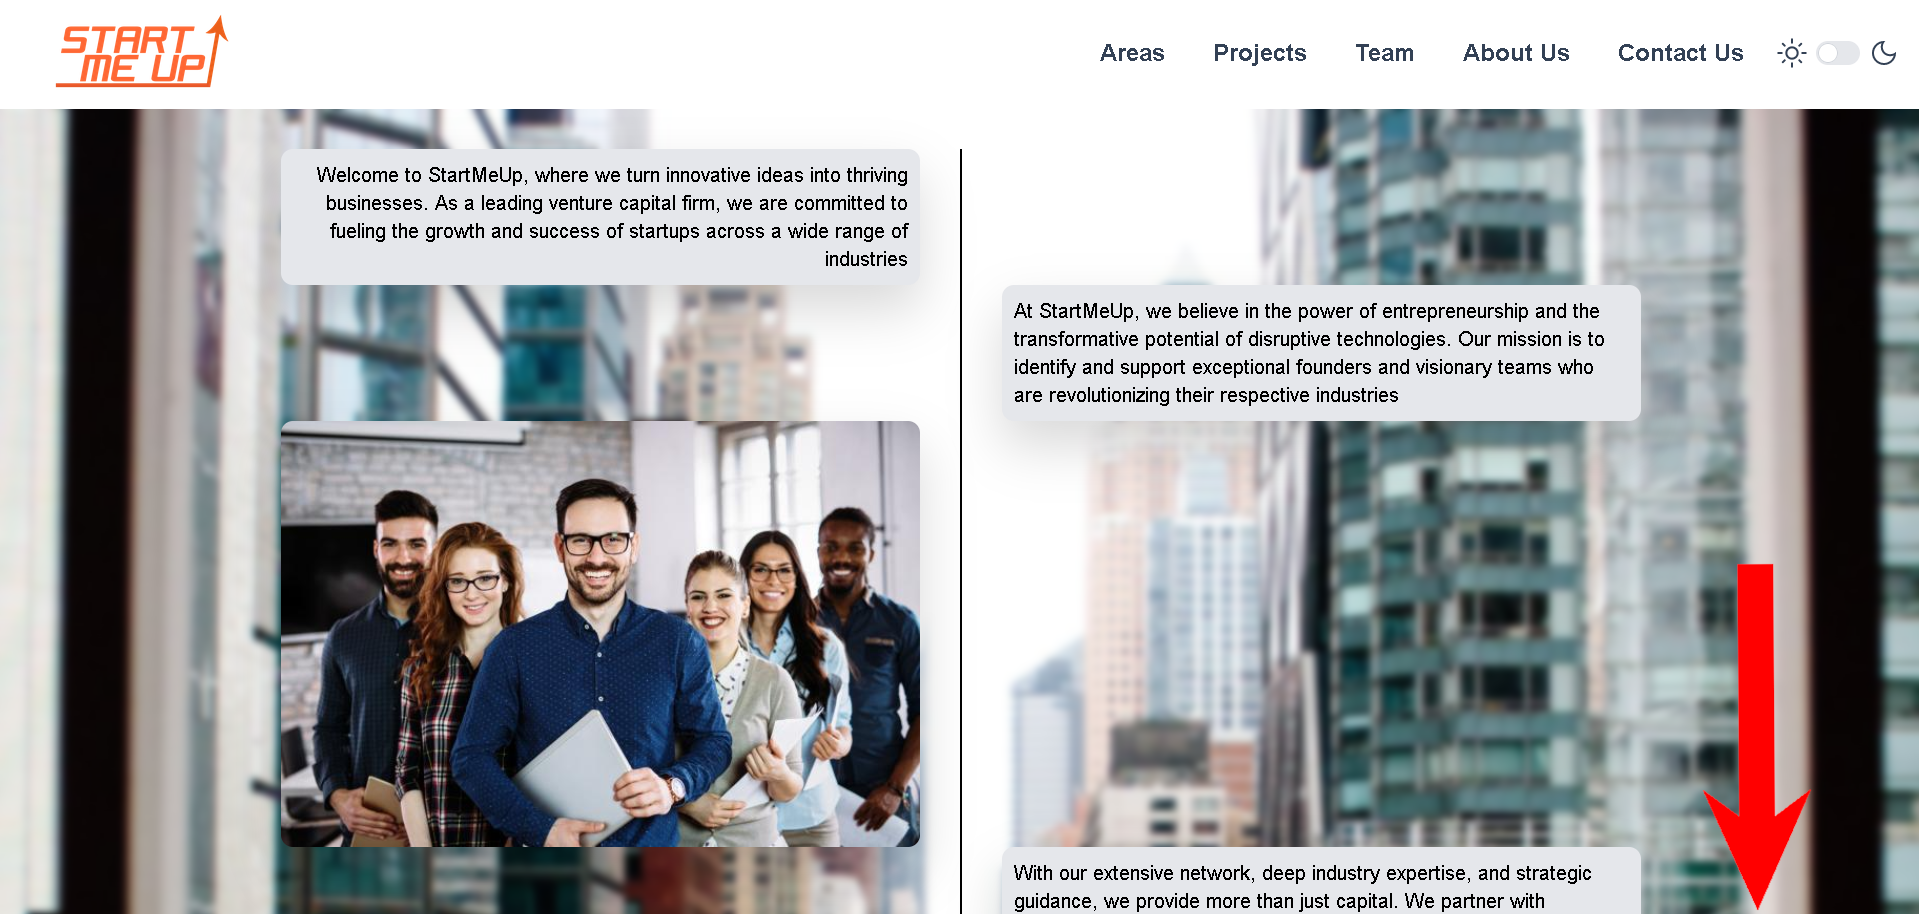
\includegraphics[width=16cm]{images/Scenarios/Scenario2/Screen1.png}}
    \caption{Scroll the Homepage}
    \label{fig:scenario2_1}
\end{figure}
\noindent
Wanting to learn more, she navigates to the "About Us" section, where she finds detailed information about the history and mission of StartMeUp.
\begin{figure}[H]
    \centering
    \setlength{\fboxsep}{0pt}\fbox{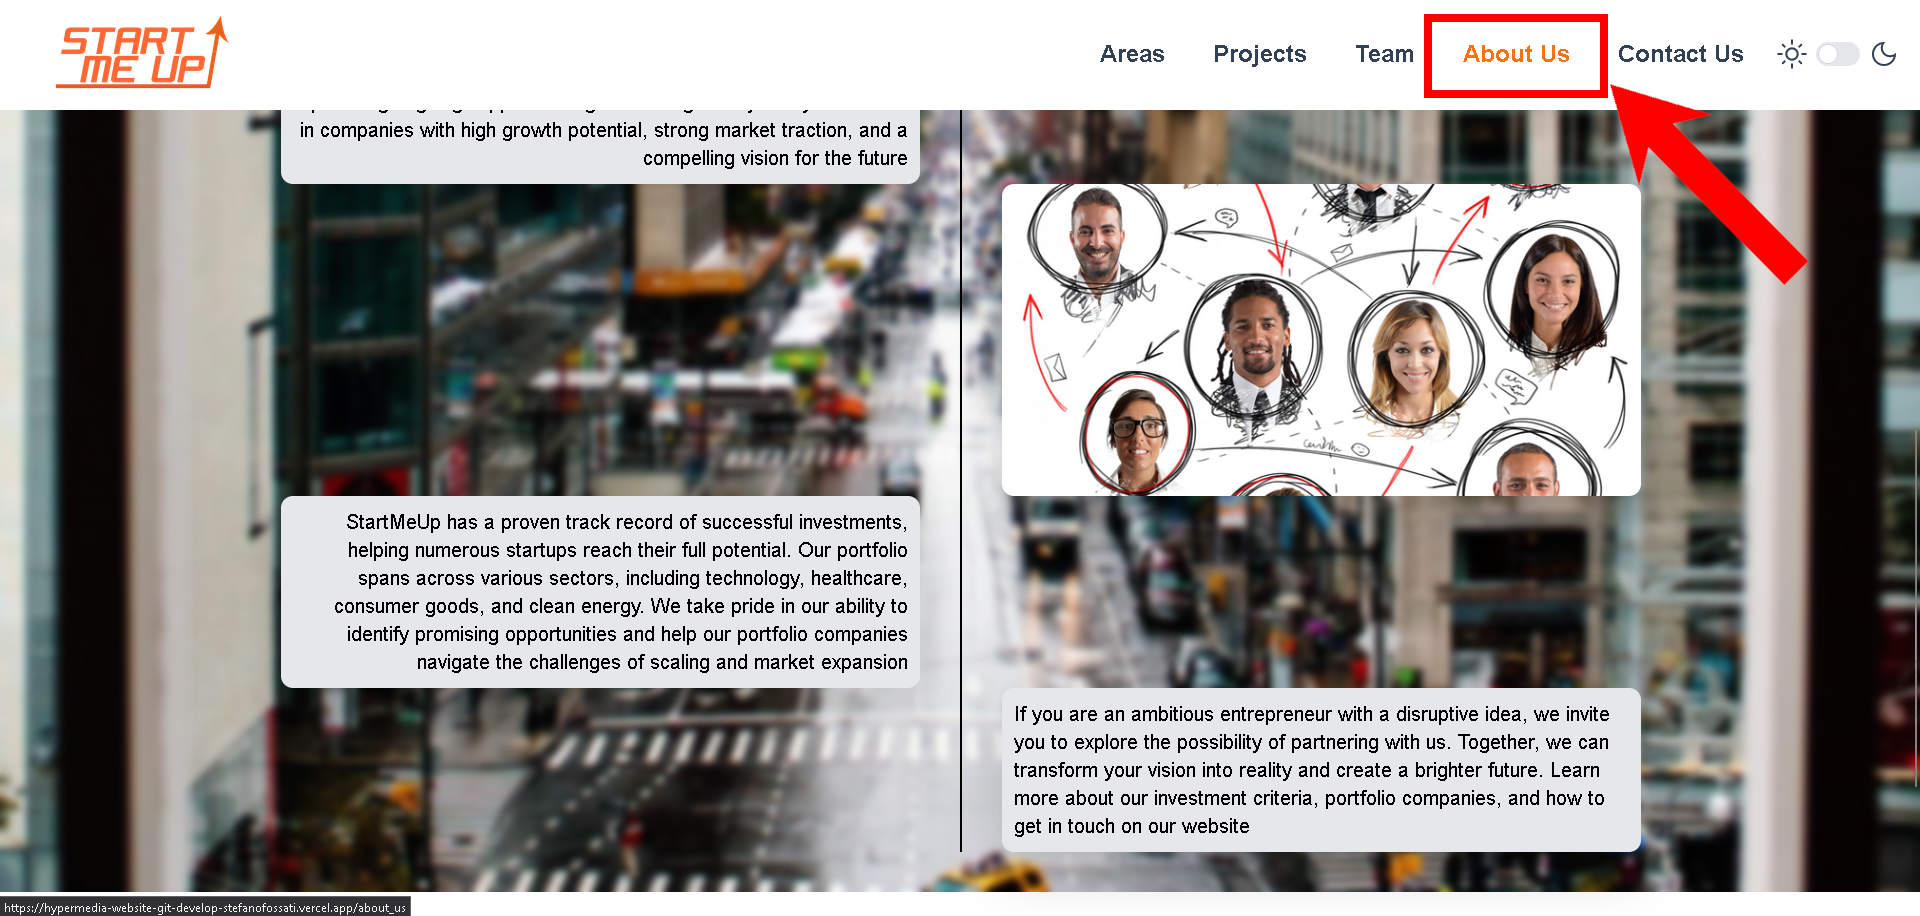
\includegraphics[width=16cm]{images/Scenarios/Scenario2/Screen2.png}}
    \caption{Click on "About Us"}
    \label{fig:scenario2_2}
\end{figure}
\noindent
Giulia is drawn to the vision of StartMeUp and identifies with their goal of promoting innovation.
\begin{figure}[H]
    \centering
    \setlength{\fboxsep}{0pt}\fbox{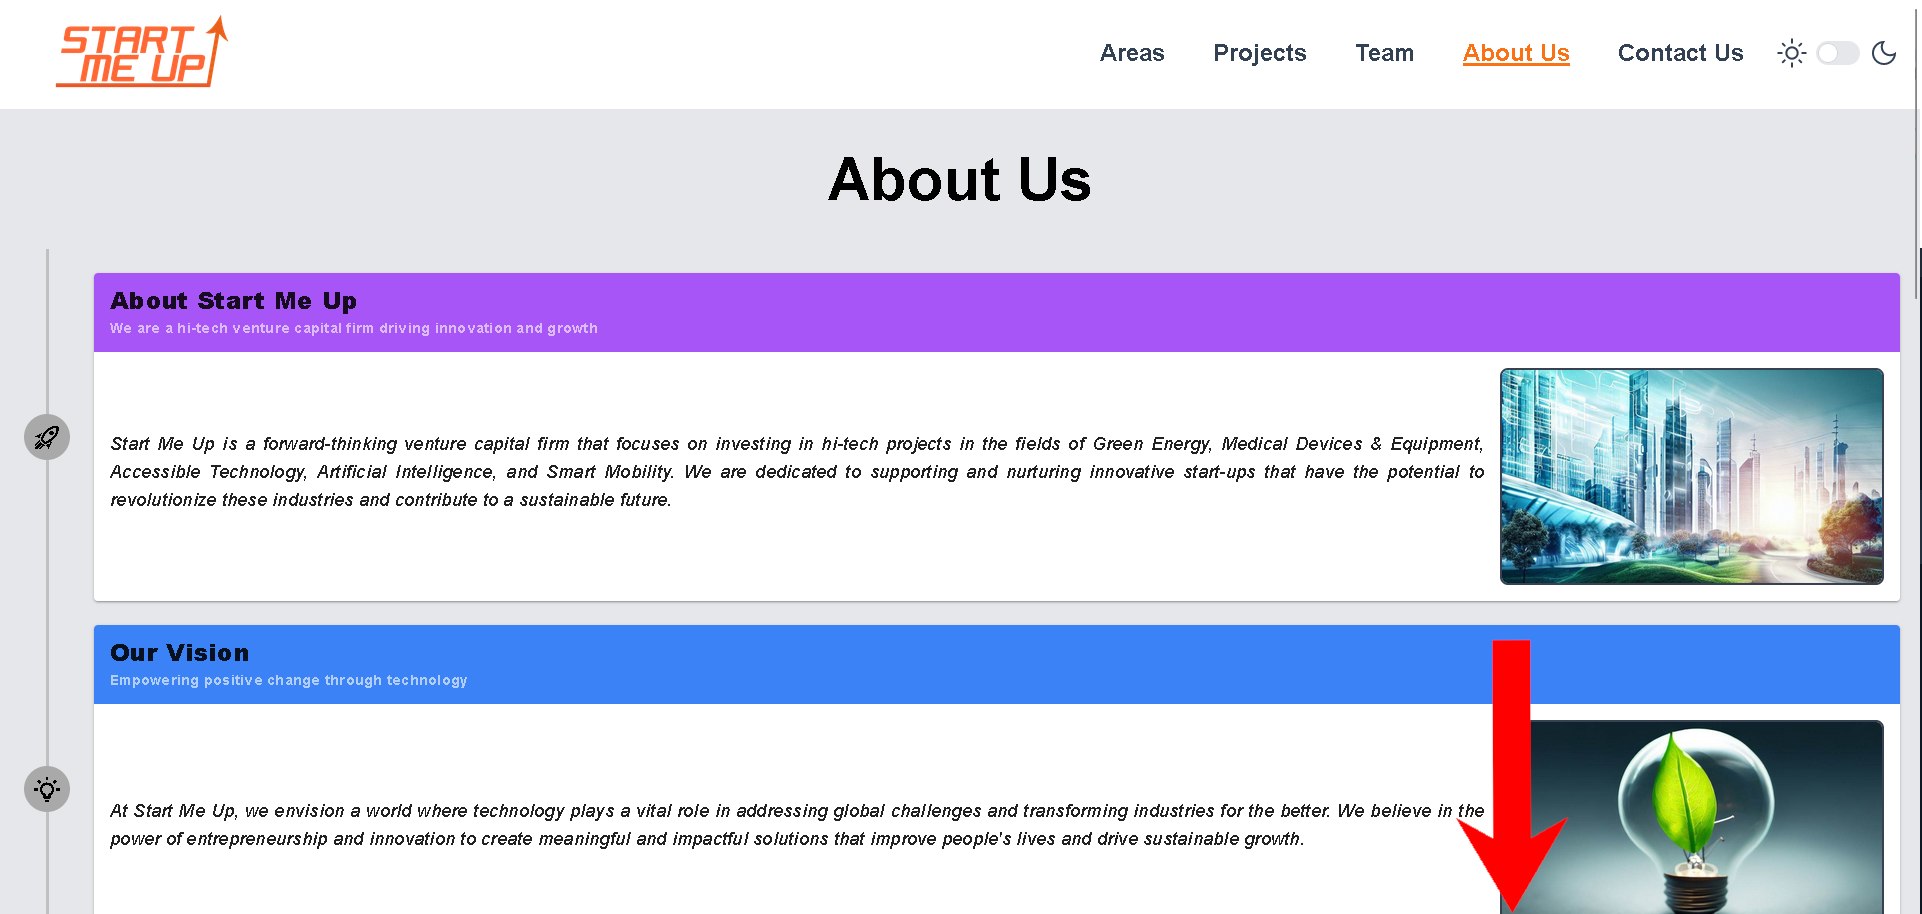
\includegraphics[width=16cm]{images/Scenarios/Scenario2/Screen3.png}}
    \caption{Scroll "About Us" page}
    \label{fig:scenario2_3}
\end{figure}
\noindent
Next, Giulia explores the "Team" section to get to know the professionals working at StartMeUp Partners.
\begin{figure}[H]
    \centering
    \setlength{\fboxsep}{0pt}\fbox{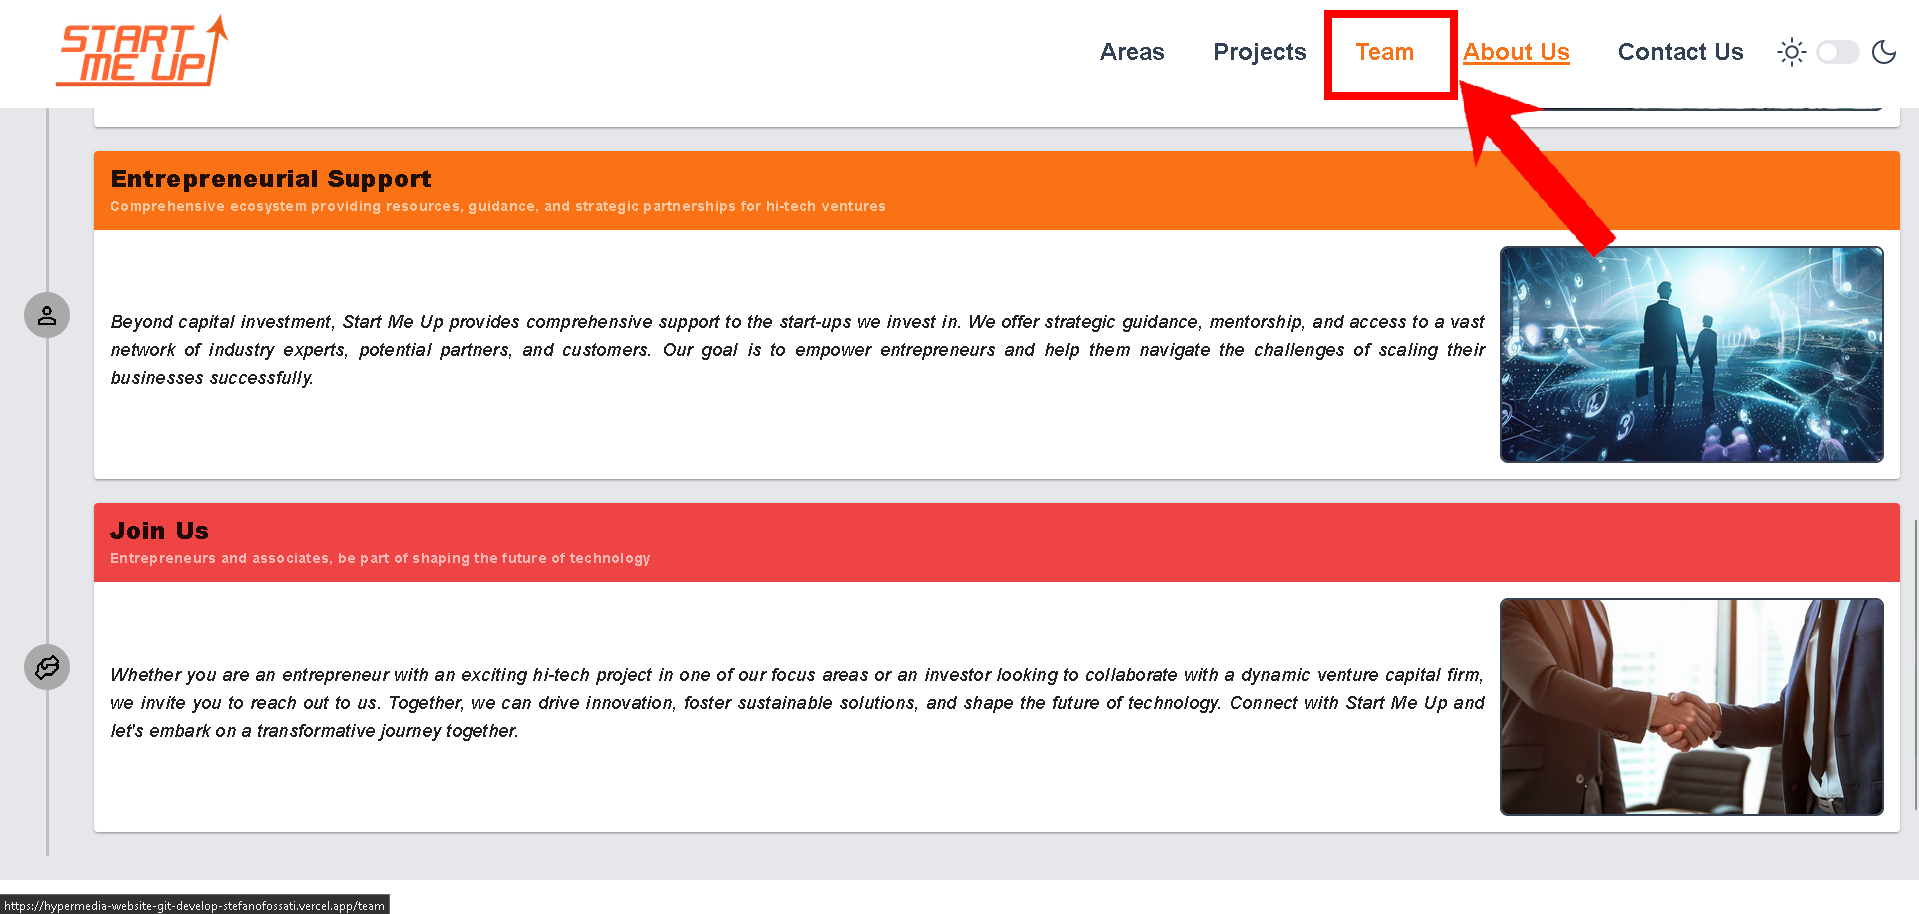
\includegraphics[width=16cm]{images/Scenarios/Scenario2/Screen4.png}}
    \caption{Click on "Team"}
    \label{fig:scenario2_4}
\end{figure}
\noindent
She finds profiles of the team members, where the experts working for the venture capital are described. So she decide to see few profiles.
\begin{figure}[H]
    \centering
    \setlength{\fboxsep}{0pt}\fbox{
\includegraphics[width=16cm]{images/Scenarios/Scenario2/Screen5.png}}
    \caption{Click on Team member's profile}
    \label{fig:scenario2_5}
\end{figure}
\noindent
After reviewing few team members, Giulia wants to try contacting the venture capital to inquire about potential opportunities to work with them going on "Contact us" page.
\begin{figure}[H]
    \centering
    \setlength{\fboxsep}{0pt}\fbox{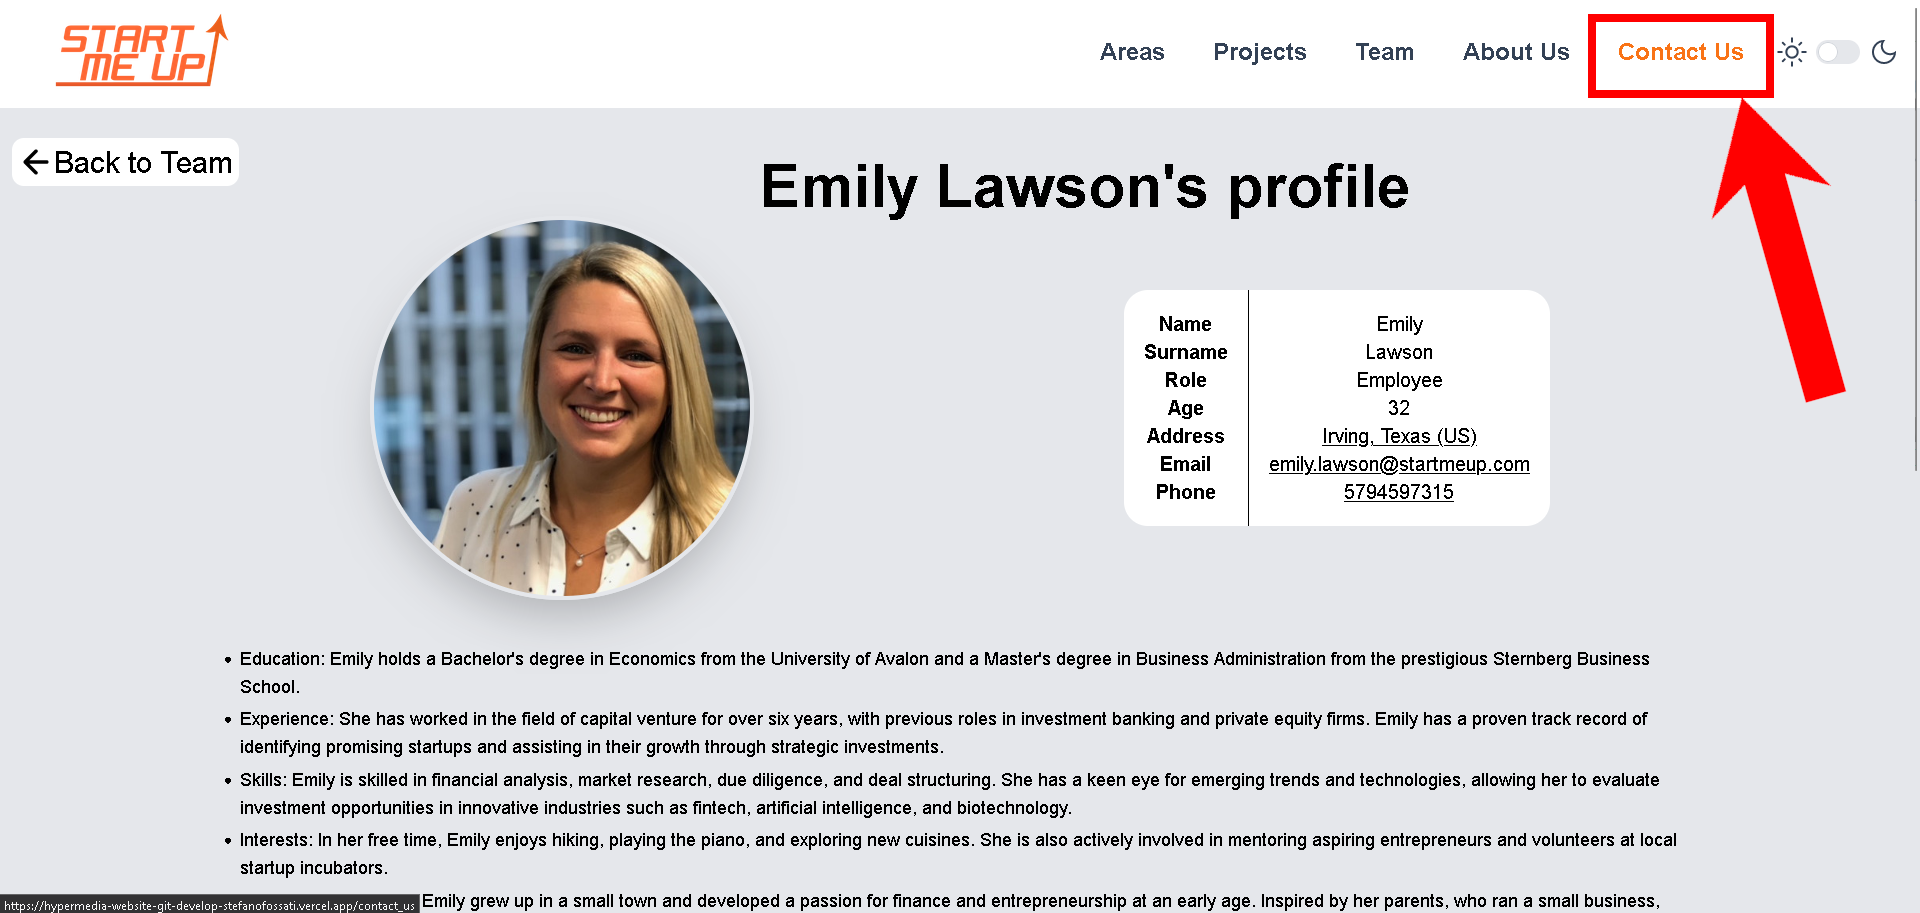
\includegraphics[width=16cm]{images/Scenarios/Scenario2/Screen6.png}}
    \caption{Click on "Contact Us"}
    \label{fig:scenario2_6}
\end{figure}
\noindent
She navigates to the "Contact Us" page and fills out the "Work With Us" form, expressing her interest and providing her relevant details.
\begin{figure}[H]
    \centering
    \setlength{\fboxsep}{0pt}\fbox{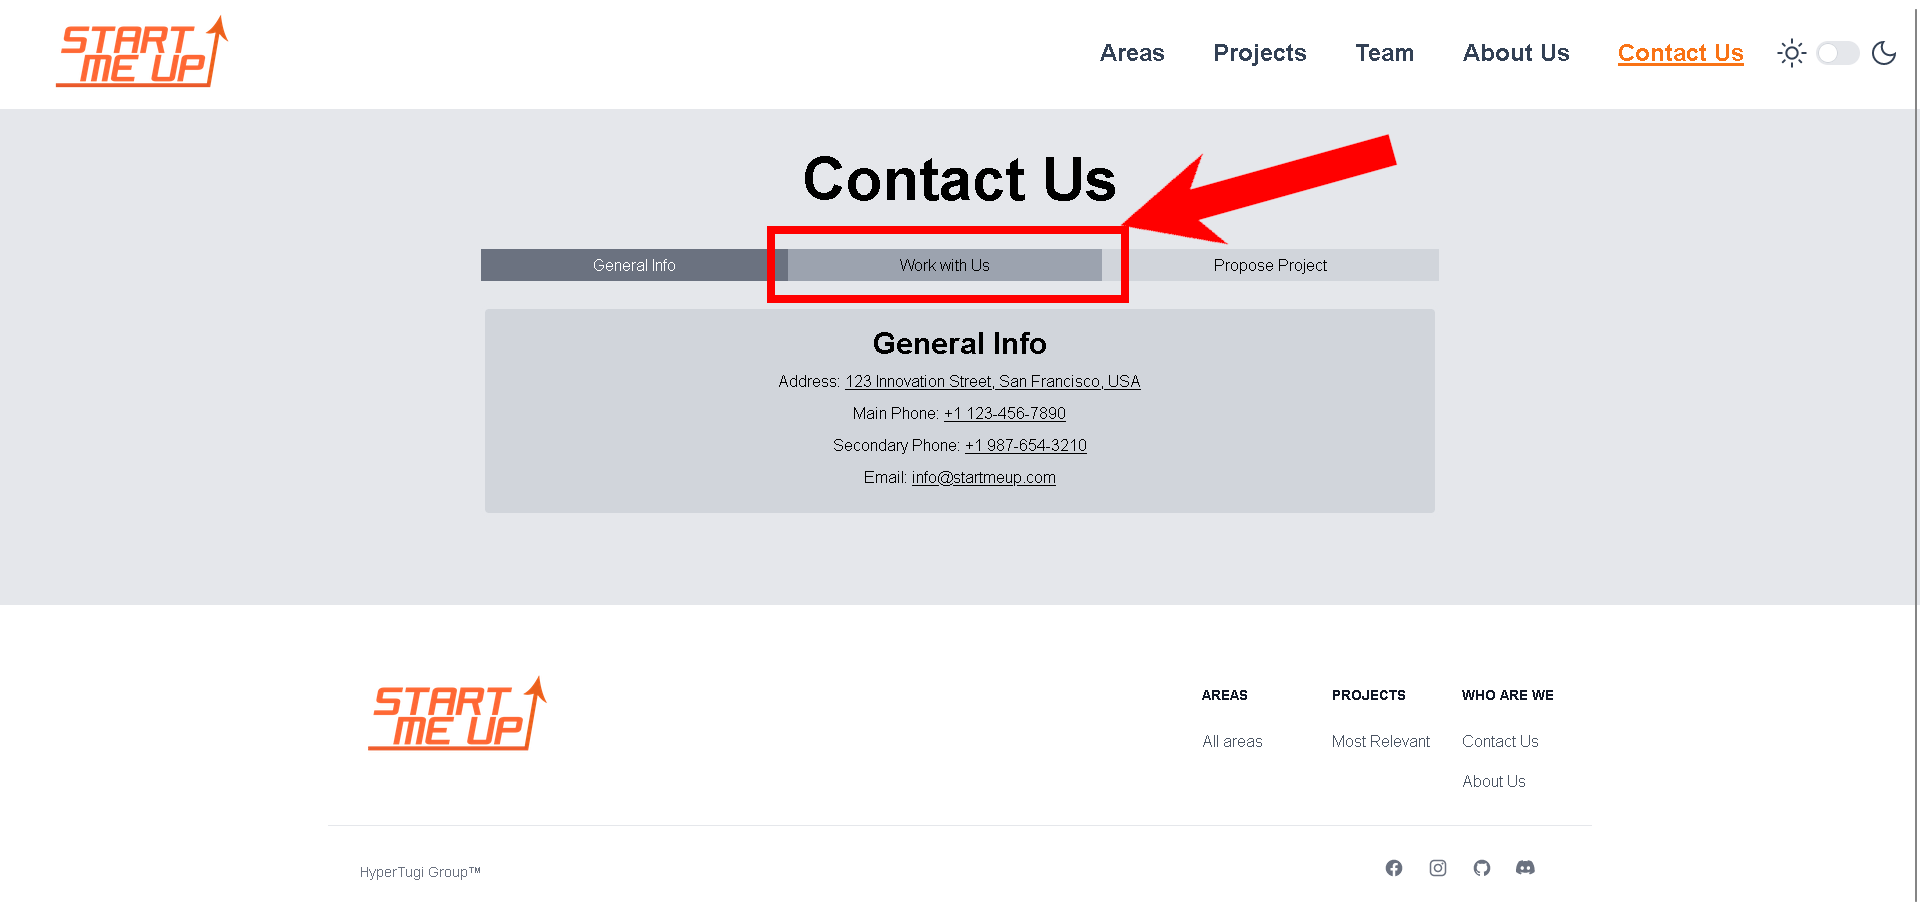
\includegraphics[width=16cm]{images/Scenarios/Scenario2/Screen7.png}}
    \caption{Click on "Work with Us"}
    \label{fig:scenario2_7}
\end{figure}
\begin{figure}[H]
    \centering
    \setlength{\fboxsep}{0pt}\fbox{
\includegraphics[width=16cm]{images/Scenarios/Scenario2/Screen8.png}}
    \caption{Fill the form and click on "Submit"}
    \label{fig:scenario2_8}
\end{figure}
\noindent
After that she has sent the form, a successful message is provided.
\begin{figure}[H]
    \centering
    \setlength{\fboxsep}{0pt}\fbox{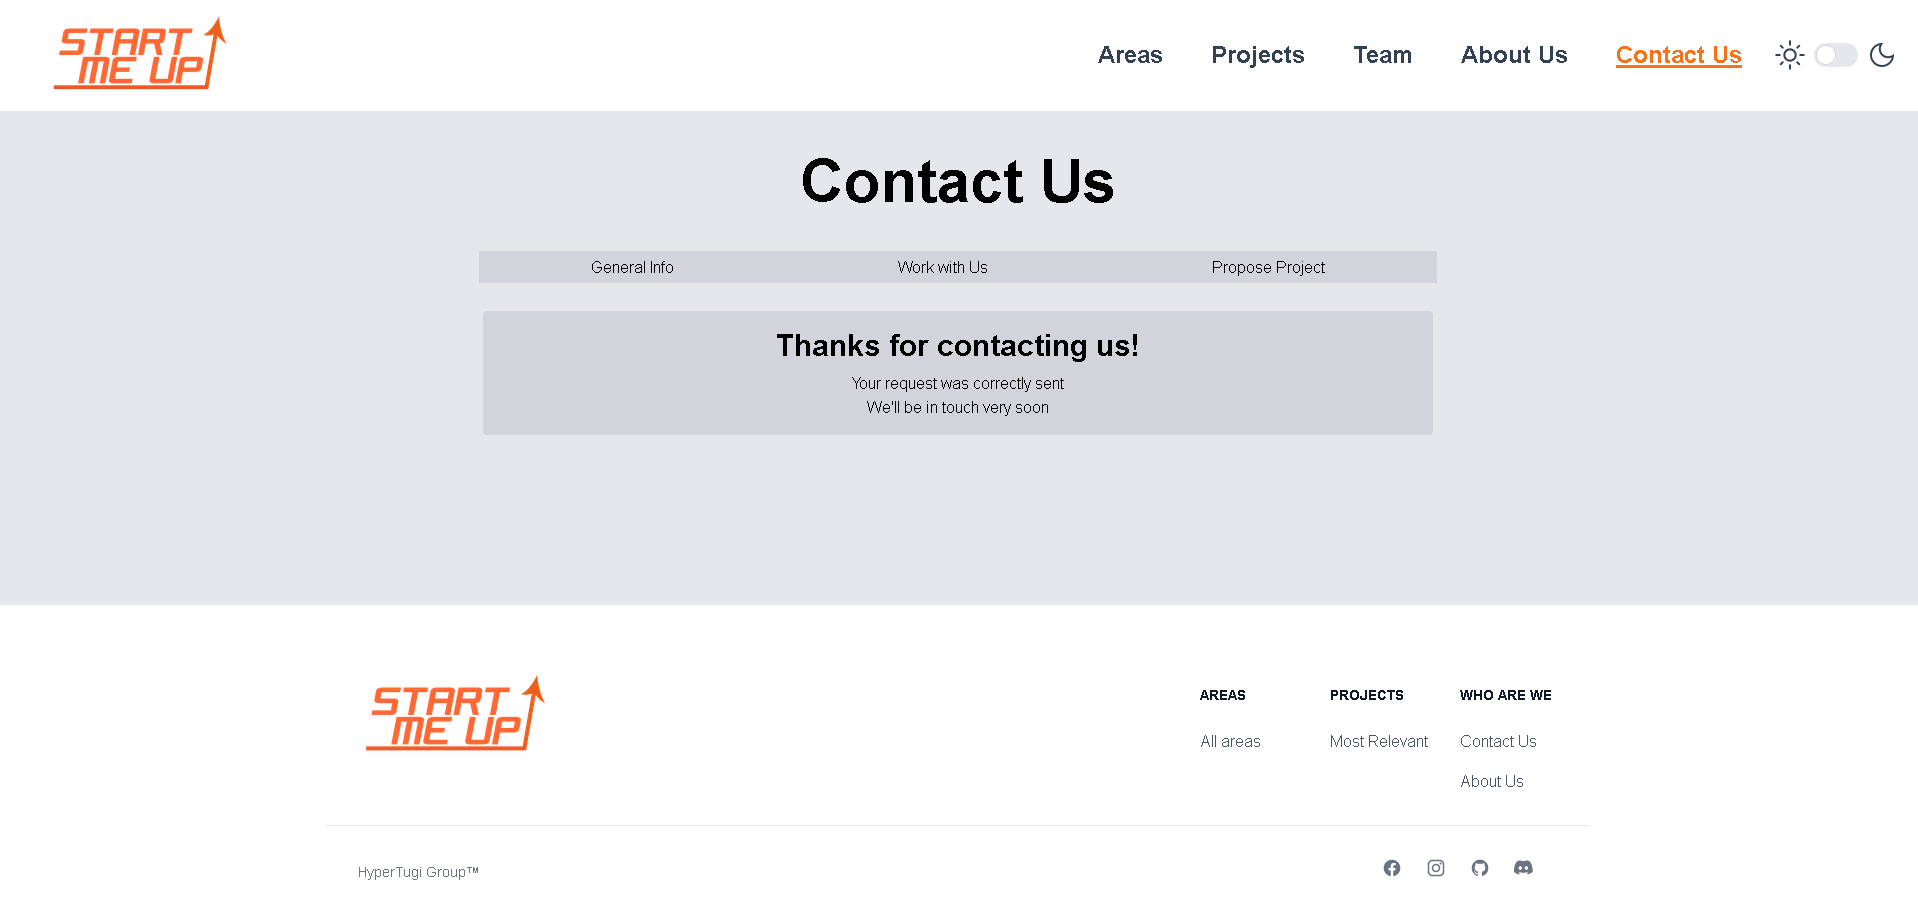
\includegraphics[width=16cm]{images/Scenarios/Scenario2/Screen9.png}}
    \caption{Form sent}
    \label{fig:scenario2_9}
\end{figure}

\subsection{Scenario 3}
Sophia is a young entrepreneur in the medical technology sector. She has developed an innovative medical device that has the potential to revolutionize the way certain diseases are diagnosed and treated. However, to move forward with her project, she needs funding. She has heard good things about a venture capital firm called " StartMeUp " and decides to visit their website to learn more.
\begin{figure}[H]
    \centering
    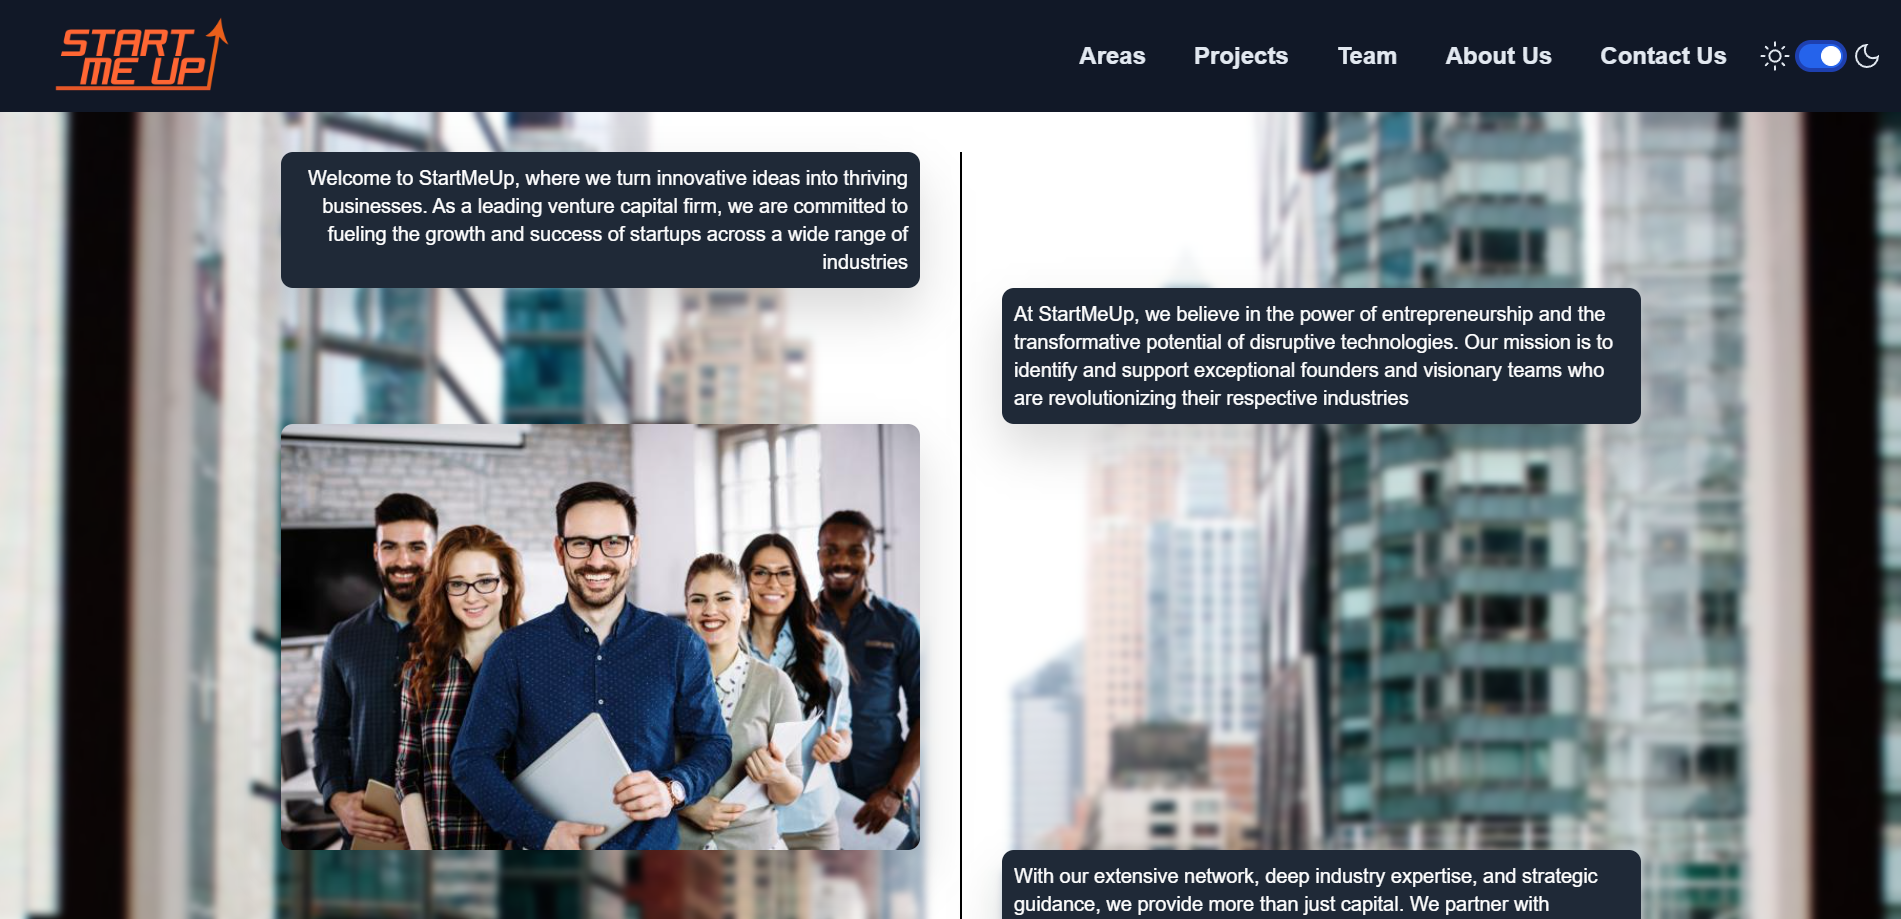
\includegraphics[width=16cm]{images/Scenarios/Scenario3/Screen1.png}
    \caption{Homepage}
    \label{fig:scenario3_1}
\end{figure}
\noindent
Sophia wants to find out if the venture capital firm invests in medical devices, so she navigates to the "Areas" section of the website.
\begin{figure}[H]
    \centering
    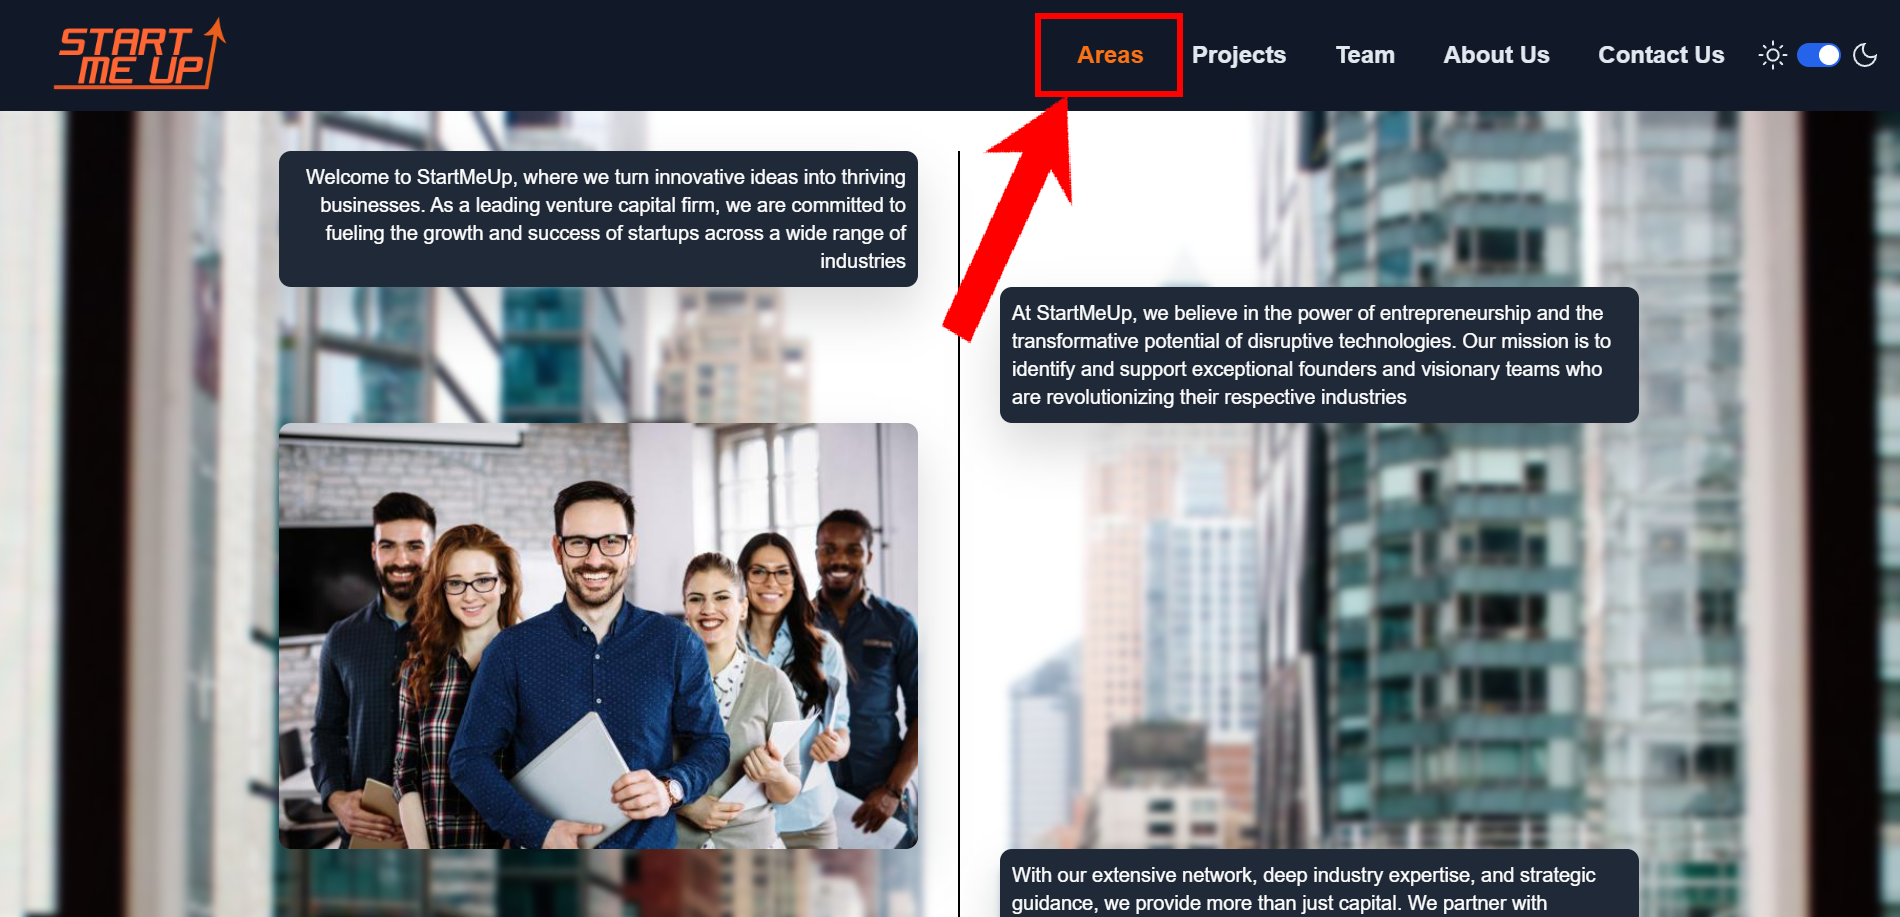
\includegraphics[width=16cm]{images/Scenarios/Scenario3/Screen2.png}
    \caption{Click on "Areas"}
    \label{fig:scenario3_2}
\end{figure}
\begin{figure}[H]
    \centering
    \includegraphics[width=16cm]{images/Scenarios/Scenario3/Screen3.png}
    \caption{Scroll the "Areas" page}
    \label{fig:scenario3_3}
\end{figure}
\noindent
She finds that Healthcare is listed as one of the areas of investment and clicks on the page.
\begin{figure}[H]
    \centering
    \includegraphics[width=16cm]{images/Scenarios/Scenario3/Screen4.png}
    \caption{Click on "Healthcare"}
    \label{fig:scenario3_4}
\end{figure}
\noindent
In the dedicated healthcare page, she reads about the specific focus that the venture capital firm has in this area. 
\begin{figure}[H]
    \centering
    \includegraphics[width=16cm]{images/Scenarios/Scenario3/Screen5.png}
    \caption{Scroll the area page}
    \label{fig:scenario3_5}
\end{figure}
\noindent
Towards the bottom, she sees a list of projects that have been funded within the healthcare sector and decides to delve deeper into the project that is most similar to her own by scrolling through them.
\begin{figure}[H]
    \centering
    \includegraphics[width=16cm]{images/Scenarios/Scenario3/Screen6.png}
    \caption{Navigate in the image gallery}
    \label{fig:scenario3_6}
\end{figure}
\begin{figure}[H]
    \centering
    \includegraphics[width=16cm]{images/Scenarios/Scenario3/Screen7.png}
    \caption{Click on "TraumaSense" project}
    \label{fig:scenario3_7}
\end{figure}
\noindent
Once she has reviewed the project, Sophia notices the information about the supervisor who oversaw that particular project. 
\begin{figure}[H]
    \centering
    \includegraphics[width=16cm]{images/Scenarios/Scenario3/Screen8.png}
    \caption{Click on supervisor's profile link}
    \label{fig:scenario3_8}
\end{figure}
\noindent
She clicks on the supervisor's profile and discovers that the person is an expert in her field. 
Recognizing the potential value of their expertise, Sophia decides to reach out directly to that person in order to seek potential funding and collaboration from the info, that are present in the team member profile.
\begin{figure}[H]
    \centering
    \includegraphics[width=16cm]{images/Scenarios/Scenario3/Screen9.png}
    \caption{Click on team member's email address}
    \label{fig:scenario3_9}
\end{figure}
\begin{figure}[H]
    \centering
    \includegraphics[width=16cm]{images/Scenarios/Scenario3/Screen10.png}
    \caption{Click on "Send" to open email editor}
    \label{fig:scenario3_10}
\end{figure}


\subsection{Scenario 4}
Alessandro is a young developer with a groundbreaking idea to make smartphones more accessible for blind people. He is seeking funding to start his activity and recently heard about a venture capital firm called " StartMeUp " during a discussion with colleagues. Intrigued by the prospect, he decides to visit the firm's website using his smartphone.
As he accesses the website, Alessandro sees a homepage that highlights key points about the firm. He reads through the description and becomes even more curious.
\begin{figure}[H]
  \centering
  \begin{minipage}[b]{0.4\textwidth}
    \includegraphics[width=7cm]{images/Scenarios/Scenario4/Screen1.png}
    \caption{Click on Homepage text box}
    \label{fig:scenario4_1}
  \end{minipage}
  \hfill
  \begin{minipage}[b]{0.4\textwidth}
    \includegraphics[width=7.2cm]{images/Scenarios/Scenario4/Screen2.png}
    \caption{Click on Navigation Bar menu}
    \label{fig:scenario4_2}
  \end{minipage}
\end{figure}
\noindent
Eager to learn more, he navigates to the "About Us" section to discover the history of StartMeUp.
There, he finds detailed information about the firm's background, mission, and values.
\begin{figure}[H]
  \centering
  \begin{minipage}[b]{0.4\textwidth}
    \includegraphics[width=7.5cm]{images/Scenarios/Scenario4/Screen3.png}
    \caption{Click on "About Us"}
    \label{fig:scenario4_3}
  \end{minipage}
  \hfill
  \begin{minipage}[b]{0.4\textwidth}
    \includegraphics[width=7.3cm]{images/Scenarios/Scenario4/Screen4.png}
    \caption{Scroll "About Us" page}
    \label{fig:scenario4_4}
  \end{minipage}
\end{figure}
\noindent
Further piquing his curiosity, Alessandro explores the "Projects" section to see the initiatives that have been funded by StartMeUp. Upon clicking on the projects, he discovers the most relevant ones and notices a tag related to accessible technology.
\begin{figure}[H]
  \centering
  \begin{minipage}[b]{0.4\textwidth}
    \includegraphics[width=7.5cm]{images/Scenarios/Scenario4/Screen5.png}
    \caption{Click on Navigation Bar menu}
    \label{fig:scenario4_5}
  \end{minipage}
  \hfill
  \begin{minipage}[b]{0.4\textwidth}
    \includegraphics[width=7.3cm]{images/Scenarios/Scenario4/Screen6.png}
    \caption{Click on "Projects"}
    \label{fig:scenario4_6}
  \end{minipage}
\end{figure}
\noindent
Intrigued, he decides to delve deeper into the firm's vision for this area by clicking on the tag. Alessandro reads the description of the accessible technology area and looks at the projects funded within that category.
\begin{figure}[H]
  \centering
  \begin{minipage}[b]{0.4\textwidth}
    \includegraphics[width=7.2cm]{images/Scenarios/Scenario4/Screen7.png}
    \caption{Click on area tag}
    \label{fig:scenario4_7}
  \end{minipage}
  \hfill
  \begin{minipage}[b]{0.4\textwidth}
    \includegraphics[width=7.2cm]{images/Scenarios/Scenario4/Screen8.png}
    \caption{Scroll the area page}
    \label{fig:scenario4_8}
  \end{minipage}
\end{figure}
\noindent
Impressed by the alignment of his idea with StartMeUp vision, Alessandro is motivated to reach out to the firm directly. He decides to contact them by phone and quickly locates the "Contact Us" section.
\begin{figure}[H]
  \centering
  \begin{minipage}[b]{0.4\textwidth}
    \includegraphics[width=7cm]{images/Scenarios/Scenario4/Screen9.png}
    \caption{Click on Navigation Bar menu}
    \label{fig:scenario4_9}
  \end{minipage}
  \hfill
  \begin{minipage}[b]{0.4\textwidth}
    \includegraphics[width=7.2cm]{images/Scenarios/Scenario4/Screen10.png}
    \caption{Click on "Contact Us"}
    \label{fig:scenario4_10}
  \end{minipage}
\end{figure}
\noindent
He clicks on the provided phone number, which initiates a call dialog on his smartphone.
\begin{figure}[H]
  \centering
  \begin{minipage}[b]{0.4\textwidth}
    \includegraphics[width=7.1cm]{images/Scenarios/Scenario4/Screen11.png}
    \caption{Click on "Main Phone" number}
    \label{fig:scenario4_11}
  \end{minipage}
  \hfill
  \begin{minipage}[b]{0.4\textwidth}
    \includegraphics[width=7.2cm]{images/Scenarios/Scenario4/Screen12.png}
    \caption{Click on "Call"}
    \label{fig:scenario4_12}
  \end{minipage}
\end{figure}



\section{DB design}
\begin{figure}[H]
    \centering
    \includegraphics[width=15cm]{images/Hyper_Design-DB E-R.png}
    \caption{E-R Diagram}
    \label{fig:ER_diagram}
\end{figure}

The main data that we need in order to represent all the pages is the following: Area, Project, Person, About Us.

\subsection{Table Description}
\subsubsection*{Area}
The Area table contains all the information that are represented in the areas page of the website. It includes a title, a main image, a description and a color. The color is used to dynamically change some class parameters into the area pages and identify to which area a project belongs with the help of a tag. The key of this table is a text field.

\subsubsection{Project Area}
This is a join table implemented from the "belong" relationship between the area and project table. It contains the information about the area of the projects.

\subsubsection*{Project}
In the Project table the key is the project title and it contains the main information that are needed to complete the website page. An important field is the gallery\_images that is an array of JSON with this structure: \{"description": "image\_description", "url": "image\_url" \}. So this allows to fetch all the information about an image that can change two components dynamically.
Another note about the description filed that is an array of text in order to separate the different paragraph of a description. One of the field contain the key of the supervisor of the project.

\subsubsection*{Team}
In the Team table all the information about the person are present. The key is an ID. The pitch field is an array of text in order to allows to do a list in the webpage.

\subsubsection*{About Us}
This table is not connected with other table because is only used to create a repetitive dynamic structure in the About Us webpage. Working just as a storage,  it contains all the elements needed to create the correct page.

\begin{figure}[H]
    \centering
    \includegraphics[width=17cm]{images/ER Diagram hyper.png}
    \caption{DB tables with attributes}
    \label{fig:DB_tables}
\end{figure}

\clearpage

\section{Annex}
\subsection{Abstract Pages}
In order to not be redundant, the Abstract Pages refer to Header and Footer without repeating every time their content. Here it is described what they contain:
\begin{itemize}
    \item Header $\rightarrow$ Links to: Homepage, All areas, Most relevant projects, All persons, Contact Us, About Us
    \item Footer $\rightarrow$ Links to: Homepage, All areas, Most relevant projects, All persons, Contact Us, About Us
\end{itemize}

\subsubsection{Areas}
\begin{figure}[H]
    \centering
    \includegraphics[width=15cm]{images/Abstract Pages/AB - Area.png}
    \caption{Abstract Page - Area}
    \label{fig:AbstractPage_Area}
\end{figure}

\begin{figure}[H]
    \centering
    \includegraphics[width=15cm]{images/Abstract Pages/AB - All areas.png}
    \caption{Abstract Page - All areas}
    \label{fig:AbstractPage_All_areas}
\end{figure}

\subsubsection{Persons}
\begin{figure}[H]
    \centering
    \includegraphics[width=15cm]{images/Abstract Pages/AB - Person.png}
    \caption{Abstract Page - Person}
    \label{fig:AbstractPage_Person}
\end{figure}

\begin{figure}[H]
    \centering
    \includegraphics[width=15cm]{images/Abstract Pages/AB - All persons.png}
    \caption{Abstract Page - All persons}
    \label{fig:AbstractPage_All_persons}
\end{figure}

\subsubsection{Projects}
\begin{figure}[H]
    \centering
    \includegraphics[width=15cm]{images/Abstract Pages/AB - Project.png}
    \caption{Abstract Page - Project}
    \label{fig:AbstractPage_Project}
\end{figure}

\begin{figure}[H]
    \centering
    \includegraphics[width=15cm]{images/Abstract Pages/AB - All projects.png}
    \caption{Abstract Page - All projects}
    \label{fig:AbstractPage_All_persons}
\end{figure}

\begin{figure}[H]
    \centering
    \includegraphics[width=15cm]{images/Abstract Pages/AB - Most relevant projects.png}
    \caption{Abstract Page - Most relevant projects}
    \label{fig:AbstractPage_Most_relevant_projects}
\end{figure}

\begin{figure}[H]
    \centering
    \includegraphics[width=15cm]{images/Abstract Pages/AB - All projects by area.png}
    \caption{Abstract Page - All projects by area}
    \label{fig:AbstractPage_All_projects_by_area}
\end{figure}

\begin{figure}[H]
    \centering
    \includegraphics[width=15cm]{images/Abstract Pages/AB - Projects by area.png}
    \caption{Abstract Page - Projects by area}
    \label{fig:AbstractPage_Projects_by_area}
\end{figure}

\subsubsection{About Us}
\begin{figure}[H]
    \centering
    \includegraphics[width=15cm]{images/Abstract Pages/AB - About Us.png}
    \caption{Abstract Page - About Us}
    \label{fig:AbstractPage_About_Us}
\end{figure}

\subsubsection{Contact Us}
\begin{figure}[H]
    \centering
    \includegraphics[width=15cm]{images/Abstract Pages/AB - Contact Us.png}
    \caption{Abstract Page - Contact Us}
    \label{fig:AbstractPage_Contact_Us}
\end{figure}

\begin{figure}[H]
    \centering
    \includegraphics[width=15cm]{images/Abstract Pages/AB - Work with Us.png}
    \caption{Abstract Page - Work with Us}
    \label{fig:AbstractPage_Work_with_Us}
\end{figure}

\begin{figure}[H]
    \centering
    \includegraphics[width=15cm]{images/Abstract Pages/AB - Propose Project.png}
    \caption{Abstract Page - Propose Project}
    \label{fig:AbstractPage_Propose_Project}
\end{figure}

%%%%
\end{document}